\documentclass[12pt,a4paper,oneside]{report}             % Single-side
%\documentclass[11pt,a4paper,twoside,openright]{report}  % Duplex


\usepackage{ifxetex}
\ifxetex
  \usepackage{fontspec}
\else
  \usepackage[T1]{fontenc}
  \usepackage[utf8]{inputenc}
  \usepackage{lmodern}
\fi

\usepackage[magyar]{babel} % Alapértelmezés szerint utoljára definiált nyelv lesz aktív, de később külön beállítjuk az aktív nyelvet.

\usepackage{combelow}
\usepackage{newunicodechar}

\newunicodechar{Ș}{\cb{S}}
\newunicodechar{ș}{\cb{s}}
\newunicodechar{Ț}{\cb{T}}
\newunicodechar{ț}{\cb{t}}

\usepackage{xcolor}

\usepackage{cmap}
\usepackage{amsfonts,amsmath,amssymb} % Mathematical symbols.
\usepackage[ruled,boxed,resetcount,linesnumbered]{algorithm2e} % For pseudocodes.
\def\algorithmcfname{algoritmus}
\makeatletter
\renewcommand{\fnum@algocf}{\AlCapSty{\AlCapFnt\thealgocf.\nobreakspace\algorithmcfname}}
\makeatother

\usepackage{booktabs} % For publication quality tables for LaTeX
\usepackage{graphicx}
\usepackage{sidecap}

%\usepackage{fancyhdr}
%\usepackage{lastpage}

\usepackage{anysize}
\usepackage{sectsty}
\usepackage{setspace}  % Ettol a tablazatok, abrak, labjegyzetek maradnak 1-es sorkozzel!

% For hyperlinks in the generated document. 
\usepackage{color}
\usepackage{listings} % For source code snippets.

%\usepackage[amsmath,thmmarks]{ntheorem} % Theorem-like environments.

\usepackage[hang]{caption}
\usepackage{scrextend}

\usepackage{indentfirst}
\usepackage{pdfpages}

\usepackage{xfrac}
\usepackage{eurosym}

\usepackage{fullpage} % a margokra is lehessen irni

\newcommand{\vigyazat}{\marginpar{\textcolor{red}{\emph{Vigy\'azat!}}}}

\usepackage{tikz}
\usepackage{verbatim}
\usetikzlibrary{arrows,shapes}
\usetikzlibrary{positioning}
\tikzset{main node/.style={circle,fill=blue!20,draw,minimum size=1cm,inner sep=0pt},
}

\definecolor{codegreen}{rgb}{0,0.6,0}
\definecolor{codegray}{rgb}{0.5,0.5,0.5}
\definecolor{codepurple}{rgb}{0.58,0,0.82}
\definecolor{backcolour}{rgb}{0.95,0.95,0.92}

\lstdefinestyle{c_sharp}{
    backgroundcolor=\color{backcolour},   
    commentstyle=\color{codegreen},
    keywordstyle=\color{magenta},
    numberstyle=\tiny\color{codegray},
    stringstyle=\color{codepurple},
    basicstyle=\footnotesize\ttfamily,
    breakatwhitespace=false,         
    breaklines=true,                 
    captionpos=b,                    
    keepspaces=true,                 
    numbers=left,                    
    numbersep=5pt,                  
    showspaces=false,                
    showstringspaces=false,
    showtabs=false,                  
    tabsize=2
}

\lstdefinelanguage{TypeScript}{
  keywords={const, let, var, if, else, while, for, switch, case, break, return},
  keywordstyle=\color{blue}\bfseries,
  ndkeywords={class, interface, type, export, async, await},
  ndkeywordstyle=\color{purple}\bfseries,
  identifierstyle=\color{black},
  sensitive=true,
  comment=[l]{//},
  morecomment=[s]{/*}{*/},
  commentstyle=\color{gray}\ttfamily,
  stringstyle=\color{red}\ttfamily,
  morestring=[b]',
  morestring=[b]"
}

% Set TypeScript code style
\lstset{
  language=TypeScript,
  basicstyle=\small\ttfamily,
  keywordstyle=\color{blue},
  commentstyle=\color{gray},
  stringstyle=\color{red},
  numbers=left,
  numberstyle=\tiny\color{codegray},
  stepnumber=1,
  numbersep=8pt,
  backgroundcolor=\color{backcolour},
  showspaces=false,
  showstringspaces=false,
  showtabs=false,
  tabsize=2,
  captionpos=b,
  breaklines=true,
  breakatwhitespace=true,
  breakautoindent=true,
  linewidth=\textwidth,
  literate={-}{-}1
}

%--------------------------------------------------------------------------------------
% Language configuration -- choose one
%--------------------------------------------------------------------------------------
%--------------------------------------------------------------------------------------
% Elnevezések
%--------------------------------------------------------------------------------------
\newcommand{\dolgozatnyelve}{\selectlanguage{magyar}}



\newcommand{\bsc}{Diplomadolgozat}
\newcommand{\msc}{Disszert\'aci\'os dolgozat}

\newcommand{\pelda}{Példa}
\newcommand{\definicio}{Definíció}
\newcommand{\tetel}{Tétel}

\newcommand{\bevezeto}{Bevezető}
\newcommand{\koszonetnyilvanitas}{Köszönetnyilvánítás}
\newcommand{\abrakjegyzeke}{Ábrák jegyzéke}
\newcommand{\tablazatokjegyzeke}{Táblázatok jegyzéke}
\newcommand{\irodalomjegyzek}{Irodalomjegyzék}
\newcommand{\fuggelek}{Függelék}


\newcommand{\englishParagraph}{
	\setlength{\parindent}{0em} % angol nyelvű dokumentumokban jellemző
	\setlength{\parskip}{0.5em} % angol nyelvű dokumentumokban jellemző
	\nonfrenchspacing
}

\newcommand{\hungarianParagraph}{
	\setlength{\parindent}{2em} % angol nyelvű dokumentumokban jellemző
	\setlength{\parskip}{0em}   % angol nyelvű dokumentumokban jellemző
	\frenchspacing
}

\newcommand{\defaultParagraph}{
	\hungarianParagraph
}  % Beállítások magyar nyelvű dolgozathoz

%--------------------------------------------------------------------------------------
% Main variables
%--------------------------------------------------------------------------------------



% Szak alapkepzes vagy mesteri
\newcommand{\szakHU}{INFORMATIKA SZAK} % SZOFTVERFEJLESZTES
\newcommand{\szakRO}{SPECIALIZAREA INFORMATIC\v A} % SPECIALIZAREA DEZVOLTAREA APLICA\c TIILOR SOFTWARE
\newcommand{\szakEN}{COMPUTER SCIENCE SPECIALIZATION} %SOFTWARE DEVELOPMENT SPECIALIZATION


\newcommand{\dolgozattipusHU}{DIPLOMADOLGOZAT} % MESTERI DISSZERT\'ACI\'O
\newcommand{\dolgozattipusRO}{LUCRARE DE DIPLOM\v A} %TEZA DE MASTERAT
\newcommand{\dolgozattipusEN}{BACHELOR THESIS} % MASTER THESIS

\newcommand{\szerzo}{\'Abr\'am Szilveszter Levente} % Szerző neve
\newcommand{\temavezetoA}{Dr. J\'anosi-Rancz Katalin Tünde} 


% Fokozatok

%Egyetemi tan\'ar/ Profesor universitar/Full Professor
%Egyetemi docens/ Conferențiar universitar/Associate professor
%Egyetemi adjunktus/Lector universitar sau Șef de lucrări /Lecturer
%Egyetemi tan\'arseg\'ed/Asistent universitar/Assistant professor


\newcommand{\temavezetoAfokozat}{Egyetemi adjunktus}% Első konzulens neve
\newcommand{\temavezetoAfokozatRo}{Lector universitar}
\newcommand{\temavezetoAfokozatEn}{Lecturer}
\newcommand{\temavezetoB}{} % Második konzulens neve; hagyd üresen, ha egy konzulensed van.
\newcommand{\cimHu}{Cronotus} % Cím
\newcommand{\cimRO}{Cronotus}
\newcommand{\cimEN}{Cronotus}
\newcommand{\ev}{2024} %az aktualis ev

%--------------------------------------------------------------------------------------
% Page layout setup
%--------------------------------------------------------------------------------------
% we need to redefine the pagestyle plain
% another possibility is to use the body of this command without \fancypagestyle
% and use \pagestyle{fancy} but in that case the special pages
% (like the ToC, the References, and the Chapter pages)remain in plane style

\usepackage{smartdiagram}
\usepackage{tikz,pgf}
\usepackage{pgfplots}
\pgfplotsset{width=7cm,compat=1.8}
\usetikzlibrary{matrix,calc,shapes}

\tikzset{
	treenode/.style = {shape=rectangle, rounded corners, draw, anchor=center, text width=5em, align=center, top color=white, bottom color=blue!20,inner sep=1ex},
	decision/.style = {treenode, diamond, inner sep=0pt},
	root/.style = {treenode, font=\Large, bottom color=red!30},
	env/.style = {treenode, font=\ttfamily\normalsize},
	finish/.style = {root, bottom color=green!40},
	dummy/.style = {circle,draw}
}


\setcounter{secnumdepth}{0}
\sectionfont{\large\upshape\bfseries}
\setcounter{secnumdepth}{2}

\sloppy % Margón túllógó sorok tiltása.
\widowpenalty=10000 \clubpenalty=10000 %A fattyú- és árvasorok elkerülése
\def\hyph{-\penalty0\hskip0pt\relax} % Kötőjeles szavak elválasztásának engedélyezése


%--------------------------------------------------------------------------------------
% Setup hyperref package
%--------------------------------------------------------------------------------------
\usepackage{xcolor}
\definecolor{bluecite}{HTML}{0875b7}
\usepackage[unicode=true,
bookmarksopen={true},
pdffitwindow=true, 
colorlinks=true, 
linkcolor=bluecite, 
citecolor=bluecite, 
urlcolor=bluecite, 
hyperfootnotes=false, 
pdfstartview={FitH},
pdfpagemode= UseNone]{hyperref}


%--------------------------------------------------------------------------------------
% Set up listings
%--------------------------------------------------------------------------------------



\definecolor{codegreen}{rgb}{0,0.6,0}
\definecolor{codegray}{rgb}{0.5,0.5,0.5}
\definecolor{codepurple}{rgb}{0.58,0,0.82}
\definecolor{backcolour}{rgb}{0.95,0.95,0.92}




\definecolor{lightgray}{rgb}{0.95,0.95,0.95}
\definecolor{darkgreen}{RGB}{3,125,80}
\lstset{frame=tb,
	language=Matlab,
	aboveskip=3mm,
	belowskip=3mm,
	showstringspaces=false,
	columns=flexible,
	basicstyle={\small\ttfamily},
	numbers=none,
	numberstyle=\tiny\color{gray},
	keywordstyle=\color{blue},
	commentstyle=\color{codegreen},
	%stringstyle=\color{mauve},
	breaklines=true,
	breakatwhitespace=true,
	tabsize=3,
	backgroundcolor=\color{lightgray},
}
\def\lstlistingname{k\'odr\'eszlet}	


%--------------------------------------------------------------------------------------
% Set up theorem-like environments
%--------------------------------------------------------------------------------------
% Using ntheorem package -- see http://www.math.washington.edu/tex-archive/macros/latex/contrib/ntheorem/ntheorem.pdf
%\swapnumbers
%\theoremstyle{plain}
%\theoremseparator{.}
\newtheorem{example}{\pelda}[section]

%\theoremseparator{.}
%\theoremprework{\bigskip\hrule\medskip}
%\theorempostwork{\hrule\bigskip}
%\theorembodyfont{\upshape}
%\theoremsymbol{{\large \ensuremath{\centerdot}}}
\newtheorem{definition}{\definicio}[section]

%\theoremseparator{.}
%\theoremprework{\bigskip\hrule\medskip}
%\theorempostwork{\hrule\bigskip}
\newtheorem{theorem}{\tetel}[section]

\newtheorem{conclusion}{Következtetés}[section]


%--------------------------------------------------------------------------------------
% Some new commands and declarations
%--------------------------------------------------------------------------------------
\newcommand{\code}[1]{{\upshape\ttfamily\scriptsize\indent #1}}
\newcommand{\doi}[1]{DOI: \href{http://dx.doi.org/\detokenize{#1}}{\raggedright{\texttt{\detokenize{#1}}}}} % A hivatkozások közt így könnyebb DOI-t megadni.

\DeclareMathOperator*{\argmax}{arg\,max}
%\DeclareMathOperator*[1]{\floor}{arg\,max}
\DeclareMathOperator{\sign}{sgn}
\DeclareMathOperator{\rot}{rot}


%--------------------------------------------------------------------------------------
% Setup captions
%--------------------------------------------------------------------------------------

\captionsetup[figure]{
	width=.75\textwidth,
	aboveskip=10pt}
\renewcommand{\captionlabelfont}{\bf}
%\renewcommand{\captionfont}{\footnotesize\it}


%--------------------------------------------------------------------------------------
% Redefine reference style
%--------------------------------------------------------------------------------------
\newcommand{\figref}[1]{\ref{fig:#1}.}
\renewcommand{\eqref}[1]{(\ref{eq:#1})}
\newcommand{\listref}[1]{\ref{listing:#1}.}
\newcommand{\sectref}[1]{\ref{sect:#1}}
\newcommand{\tabref}[1]{\ref{tab:#1}.}





%--------------------------------------------------------------------------------------
% Table of contents and the main text
%--------------------------------------------------------------------------------------
\begin{document}
	
% CIMOLDALAK
%~~~~~~~~~~~~~~~~~~~~~~~~~~~~~~~~~~~~~~~~~~~~~~~~~~~~~~~~~~~~~~~~~~~~~~~~~~~~~~~~~~~~~~
	%--------------------------------------------------------------------------------------
%	A magyar cimoldal
%--------------------------------------------------------------------------------------
\begin{titlepage}
	\begin{center}
	
		\large{\bfseries SAPIENTIA ERDÉLYI MAGYAR TUDOMÁNYEGYETEM} \\
		\large{\bfseries MAROSVÁSÁRHELYI KAR,} \\
		\large{\bfseries \szakHU} \\[2.5cm]
			\begin{center}
			
\includegraphics[scale=2]{images/sapientia-hu}
		\end{center}
		\vspace{0.4cm}
		\Large{\Large  \cimHu}\\[0.8cm]
		\vspace{0.2cm}
		\textsc{\Large \bfseries \dolgozattipusHU}\\[2.5cm]
		
		{
			\large
		
			\renewcommand{\arraystretch}{0.85}
			\begin{tabular}{cc}
				 \makebox[6.5cm]{Témavezető:} & \makebox[6.5cm]{Végzős hallgató:} \\ \noalign{\smallskip}
				 \makebox[6.5cm]{\temavezetoA,} & \makebox[6.5cm]{\szerzo} \\ {\temavezetoAfokozat}
			\end{tabular}
		}
		
		\vfill
		{\large \bfseries \ev}
	\end{center}
\end{titlepage}
	%--------------------------------------------------------------------------------------
%	The title page RO
%--------------------------------------------------------------------------------------

\begin{titlepage}
	\begin{center}
	
		\large{\bfseries UNIVERSITATEA SAPIENTIA DIN CLUJ-NAPOCA} \\
		\large{\bfseries FACULTATEA DE ȘTIINȚE TEHNICE ȘI UMANISTE,} \\
		
		\large{\bfseries \szakRO} \\[2.5cm]
		
			\begin{center}
			
\includegraphics[scale=2]{images/sapientia-ro}
		\end{center}
		
		\vspace{0.4cm}
		
	
		
		\Large{\Large \cimRO}\\[0.8cm]
		\vspace{0.5cm}
		\textsc{\Large \bfseries \dolgozattipusRO}\\[2.5cm]
		
		{
			\large
		
			\renewcommand{\arraystretch}{0.85}
			\begin{tabular}{cc}
				 \makebox[6.5cm]{Coordonator științific:} & \makebox[6.5cm]{Absolvent:} \\ \noalign{\smallskip}
				 \makebox[6.5cm]{\temavezetoA,} & \makebox[6.5cm]{\szerzo} \\
				 {\temavezetoAfokozatRo}
			\end{tabular}
		}
		
		\vfill
		{\large \bfseries \ev}
	\end{center}
\end{titlepage}
	%--------------------------------------------------------------------------------------
%	The title page EN
%--------------------------------------------------------------------------------------

\begin{titlepage}
	\begin{center}
	
		\large{\bfseries SAPIENTIA HUNGARIAN UNIVERSITY OF TRANSYLVANIA} \\
		\large{\bfseries FACULTY OF TECHNICAL AND HUMAN SCIENCES} \\
		\large{\bfseries \szakEN} \\[2.5cm]
		
			\begin{center}
			
\includegraphics[scale=2]{images/sapientia-en}
		\end{center}
		\vspace{0.4cm}
		\Large{\Large  \cimEN}\\[0.8cm]
		\vspace{0.5cm}
		\textsc{\Large \bfseries \dolgozattipusEN}\\[2.5cm]
		
		{
			\large
	
			\renewcommand{\arraystretch}{0.85}
			\begin{tabular}{cc}
				 \makebox[6.5cm]{Scientific advisor:} & \makebox[6.5cm]{Student:} \\ \noalign{\smallskip}
				 \makebox[6.5cm]{\temavezetoA,} & \makebox[6.5cm]{\szerzo} \\
				 {\temavezetoAfokozatEn}
			\end{tabular}
		}
		
		\vfill
		{\large \bfseries \ev}
	\end{center}
\end{titlepage}
	
	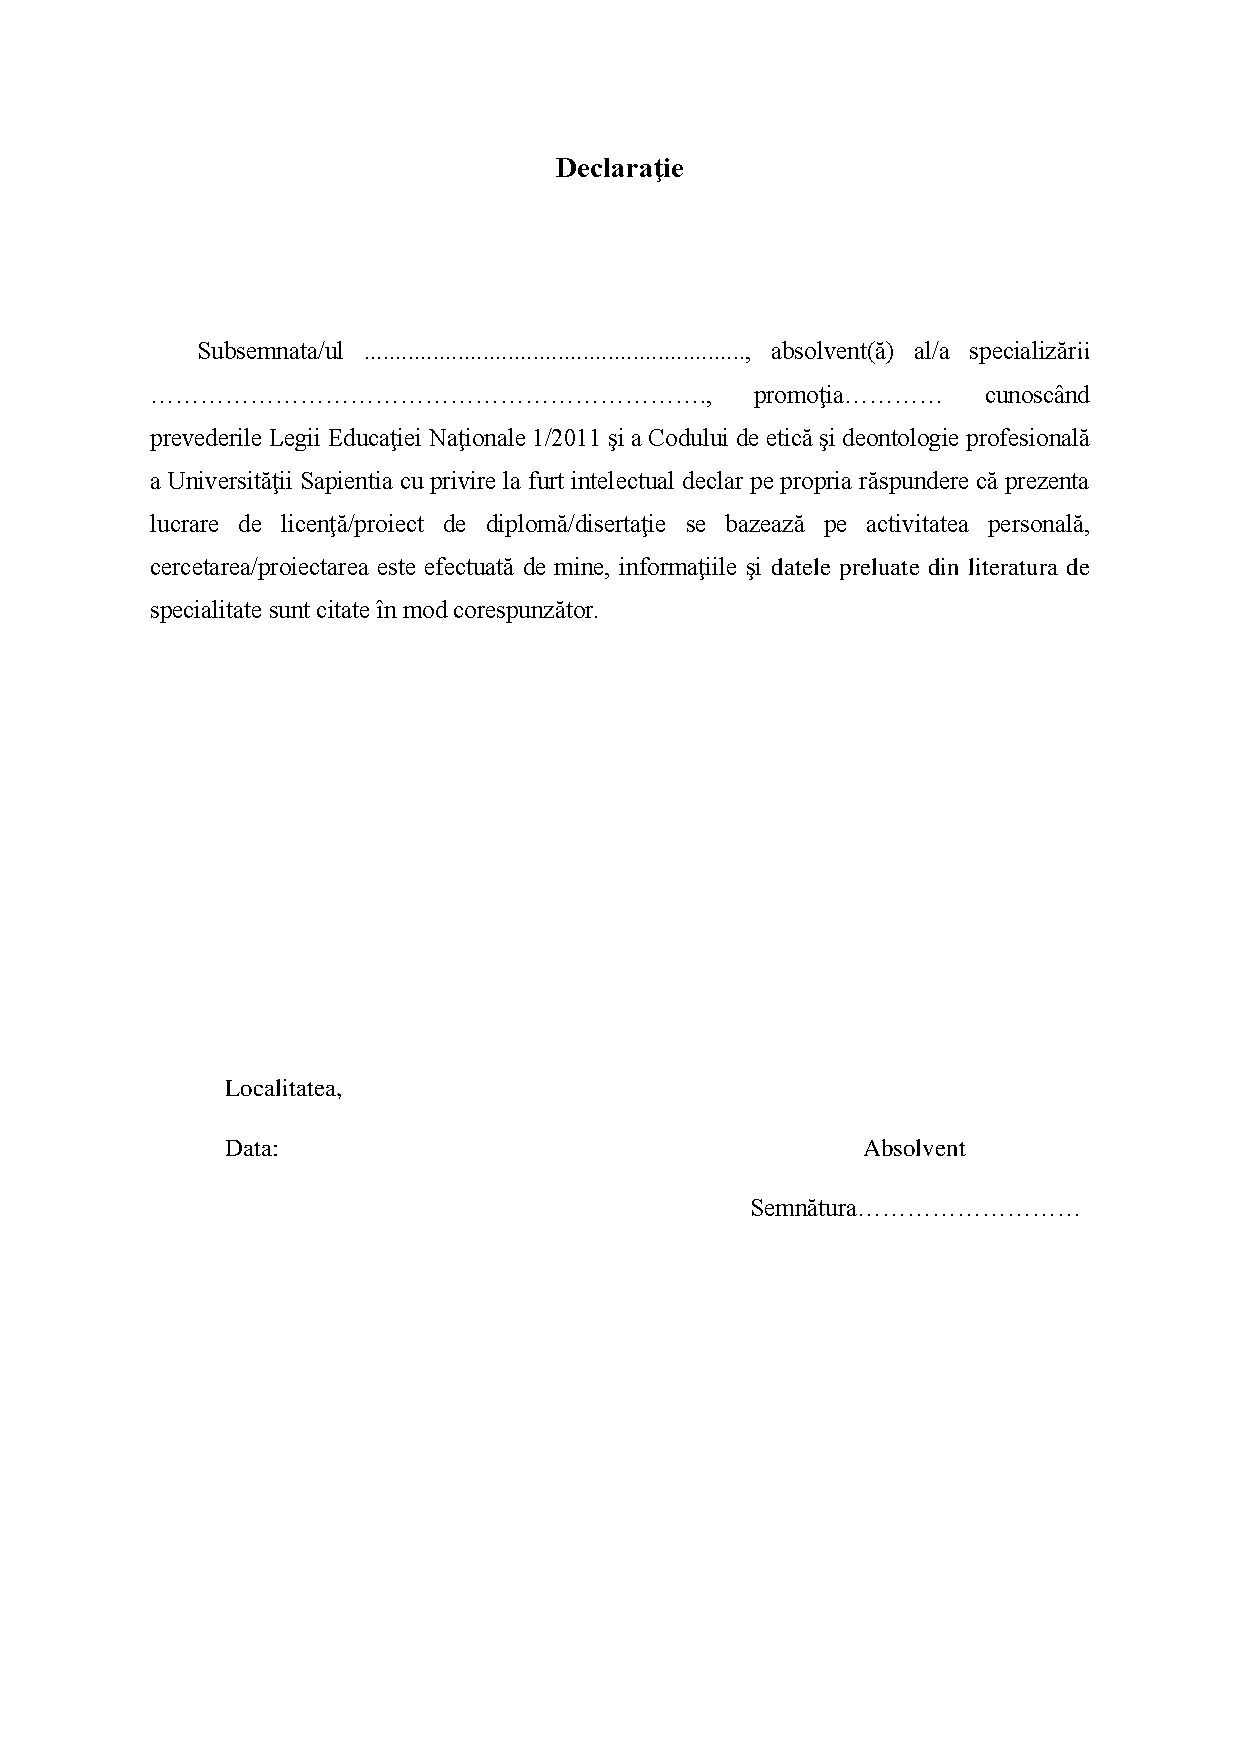
\includepdf[pages={1}]{content/Declaratie.pdf}
	\pagenumbering{gobble}

\selectlanguage{magyar}
\hungarianParagraph

%----------------------------------------------------------------------------
% Abstract in Hungarian
%----------------------------------------------------------------------------
\chapter*{Kivonat}
A mozgás és a különböző sportok űzése szerves részét képezik az emberek mindennapi
  életének. Ahhoz, hogy egészségesen élhessünk, mindannyian más és más sportokat választunk,
  melyekbe naponta energiát és időt fektetünk. A mozgás nem csak fizikai, de szellemi
  egészségünkre is nagy hatással van, továbbá az, hogy kikkel sportolunk, nagymértékben
  meghatározza a mozgással eltöltött időnk minőségét\cite{warner2017yielding}. Mindenki számára fontos a közösség, úgy a
  magánéletben, mint a sportolásban is. A legnagyobb kihívást sokszor az jelenti, hogy
  megtaláljuk az ideális társaságot és a közösen eltöltött idő valóban minőségi legyen.
  
  Dolgozatom célja, egy olyan alkalmazás bemutatása, amely a sportolásra ösztönöz
  mindenkit és segít a sportolói közösség kialakításában is.
  
  A Cronotus egy olyan internetes felületet biztosít, ahol az emberek könnyedén
  kiküszöbölhetik a sportoláshoz szükséges társaság hiányában felmerülő problémát. Lehetőséget
  biztosít sportesemények szervezésére, illetve ezek böngészésére, hogy biztosak lehessünk abban,
  hogy többé senki nem marad otthon azért, mert nem volt akivel sportolni menjen. A projekt
  továbbá szem előtt tartja azt is, hogy egyes események könnyedén követhetőek legyenek,
  lehetőséget biztosít a szervezőknek arra, hogy naprakész információkkal lássák el a sportolókat,
  ami segíthet a közösségnek abban, hogy
  a számukra legmegfelelőbb eseményeket találják meg.



\vfill
Kulcsszavak: sport, sportesemény, szervezés, koordinálás, közösség
\clearpage
\selectlanguage{romanian}

%----------------------------------------------------------------------------
% Abstract in Romanian
%----------------------------------------------------------------------------
\chapter*{Rezumat}
Exercițiile fizice și practicarea diferitelor sporturi fac parte integrantă din viața de zi cu zi a oamenilor.
  Pentru a avea o viață sănătoasă, cu toții alegem diferite sporturi,
  în care investim energie și timp în fiecare zi. Exercițiile fizice nu au numai beneficii fizice, ci au efecte semnificative și asupra sănătății mintale,
  iar oamenii cu care facem sport pot determina calitatea timpului pe care îl petrecem făcând mișcare.\cite{warner2017yielding} Comunitatea este importantă
  pentru toată lumea, atât în viața personală, cât și în activitățile sportive. Cea mai mare problemă este adesea aceea de a găsi compania potrivită și de a face timpul petrecut împreună cu aceasta să fie cu adevărat de calitate.
  
  Scopul tezei este de a prezenta o aplicație care încurajează oamenii să facă sport
  tuturor și, de asemenea, ajută la construirea unei comunități de sportivi.
  
  Cronotus oferă o platformă online prin care oamenii pot cu ușurință
  să depășească problema de a nu avea companie pentru a face sport. Aplicația vă permite organizarea, căutarea evenimentelor sportive, 
  astfel încât să ne asigurăm că nimeni nu rămâne acasă pentru că nu are cu cine să iasă la sport. 
  Proiectul își propune, de asemenea, să facă anumite evenimente ușor de urmărit,
  oferindu-le organizatorilor posibilitatea de a oferi informații actualizate sportivilor, care să ajute comunitatea să
  să găsească evenimentele care sunt cele mai potrivite pentru ei.


\vfill
Cuvinte cheie: sport, eveniment sportiv, organizare, coordonare, comunitate
\clearpage
\selectlanguage{english}
%\englishParagraph

%----------------------------------------------------------------------------
% Abstract in English
%----------------------------------------------------------------------------
\chapter*{Abstract}
Physical activity and practicing various sports are an integral part of people's everyday lives.
  In order to live a healthy life, we all choose different sports,
  in which we invest energy and time every day. Physical exercise has proven to not only havephysical benefits, but also significant effects on mental health,
  furthermore the people we do sports with can determine the quality of the time we spend exercising.\cite{warner2017yielding} Choosing the right community for doing sports and everyday 
  activities is a challange that everyone faces, since it great impact on our lives.
  
  The purpose of this is thesis is providing a platform that serves as a middleware for people that want to connect with others,
  and fight the problem of not having company to exercise.
  
  Cronotus provides an online platform where people can easily
  overcome the problem of not having company to exercise. The application allows one to organize, search for sports events,
  so that we can make sure that no one is left home because they had no one to go out with. 
  The project also aims to make certain events easy to follow,
  providing organizers with the opportunity to provide up-to-date information to athletes, which can help the community
  to find the events that are most suitable for them.

\vfill
Keywords: sport, sporting event, organization, coordination, community, social
\clearpage
\dolgozatnyelve
\defaultParagraph
 
% Tartalomjegyzek
%~~~~~~~~~~~~~~~~~~~~~~~~~~~~~~~~~~~~~~~~~~~~~~~~~~~~~~~~~~~~~~~~~~~~~~~~~~~~~~~~~~~~~~
	\pagenumbering{arabic}
	\setcounter{page}{9}
	\tableofcontents\vfill

% A diplomadolgozat lenyegi resze
%~~~~~~~~~~~~~~~~~~~~~~~~~~~~~~~~~~~~~~~~~~~~~~~~~~~~~~~~~~~~~~~~~~~~~~~~~~~~~~~~~~~~~~

% ajánlott külön file-okba írni az egyes fejezeteket, ugyanis úgy jobban át lehet látni.



	%----------------------------------------------------------------------------
\chapter{Bevezető}%\addcontentsline{toc}{chapter}{Bevezető}
%----------------------------------------------------------------------------

Annak ellenére, hogy az információ közlése és elérése napjainkban rendkívül gyors és olcsó, mégis előfordul, hogy alapvető tevékenységeket igen csak maradi módon kezelnek az emberek. Többek között idetartozik egyes sportesemények koordinálása is. A résztvevők gyakran hajlamosak egy nem erre a célra készített platformra hagyatkozni, ami természetesen nem mindig működik úgy, ahogy ideális lenne. Ennek eredményeként megtörténik, hogy lemaradnak az emberek olyan információkról, ami egyébként releváns lett volna számukra.

A Cronotus projekt ennek a problémának a megoldását egy ingyenes és könnyen kezelhető platfrom biztosításával közelíti meg, ami arra törekszik, hogy kiküszöbölje az esetelges információk elvesztését, vagy akár figyelmen kívül hagyását.

A dolgozat elsősorban bemutatja a projekt általános működését, párhuzamba helyezi más ehhez hasonló internetes platformokkal, szemünk elé tárja az esetleges előnyöket és hátrányokat más szolgáltatásokkal szemben.

A továbbiakban a dolgozat ismerteti velünk mélyebben a Cronotus szerkezetét, ahol felépítés szerinti rétegekre bontja, majd ezeket részletekbe bocsátkozva tárgyalja. Bemutatja azt, hogy hogyan működik a web kliens-t kiszolágló szerver, milyen biztonsági intézkedéseket biztosít, illetve hogyan kezeli a felmerülő hibákat. Betekintést biztosít abba, hogy hogyan érkezik el a kívánt információ az adatbázistól egészen a felhasználó felületig.

A következő fejezetek segítségével szeretném bemutatni a felhasznált eszközöket és módszereket, melyek elősegítik a Crontous helyes működését. Végezetül egy következtetést vonok le, illetőleg továbbfejlesztési lehetőségeket tárok az olvasó elé, melyek fényt derítenek a projekt jövőbeli élettartamára.

A paltform készítése 2023 októberében kezdődött a Codespring szoftverfejlesztő cég koordinálásával. Megemlítendő, hogy a felhasznált technológiák visszatükrözik azt a tudást, amit a Marosvásárhelyi Codespring Mentorprogram keretein belül sajátíthattam el, ami 2022 őszi időszakában vette kezdetét. A projektet a koordináló cég segítségével egyedül fejlesztettem.

Az alkalmazás neve, azaz a Cronotus, egy összetett lingvisztikai ihletből merített szó. A név első fele a görög mitológiai Krónosztól származik, akit az idő isteneként ismerünk, míg a név második fele a ``mozgás'' szó latin fordításából, a 'motus' szóból ered.

	\chapter{A Cronotus projekt}

  A Cronotus projekt célja egy olyan internetes felület biztosítása, ahol az emberek könnyedén megtalálhatják a számukra legmegfelelőbb 
  sportolási lehetőségeket. Mindez egy webalkalmazás formájában valósul meg, ahová felhasználóként regisztrálva tudunk interakcióba lépni
  az elérhető sporteseményekkel, szervezőkkel.

  A rendszer igyekszik azt elérni, hogy különböző módokon hozza közelebb egymáshoz a sportolni vágyó felhasználókat. Abban az esetben, ha 
  létezik egy megfelelő sportesemény könnyedén csatlakozni lehet hozzá, ha meg nem, akkor lehetőség van egy megfelelő új esemény létrehozására.

\section{Piackutatás}
  Ahhoz, hogy jobban megérthessük a társaság hiánya okozta sportolási nehézségeket, az alábbiakban egy általunk végzett felmérést fogunk megvizsgálni.
  A felmérésben összegyűjtött adatok legfőképpen a erdélyi magyar fiataloktól származnak, korosztály szempontjából legjellemzőbben a 
  19-25 éves korig terjedő egyénekre vonatkoznak. A kutatáson 30 fő vett részt.

  \newpage

  Első sorban megbizonyosodtunk arról, hogy a fiatalok igenis érdeklődnek a sportok iránt. A felmérés kimutatta azt, hogy az egyének 90\%-a
  havonta legalább két alkalommal sportol, 36\%-uk heti szinten, míg 15\%-uk hetente többször is, ahogy ez a \ref{fig:how_much_do_people_sport}-es ábrán is látható.

  \begin{figure}[ht]
    \centering
    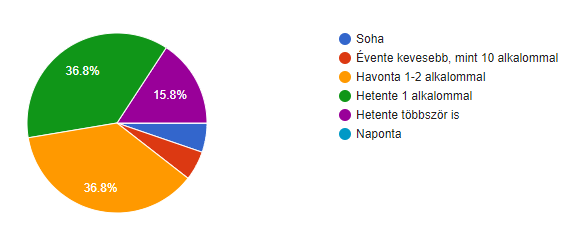
\includegraphics[width=0.8\textwidth]{./images/Screenshot 2024-04-12 162623.png}
    \caption{Mennyit sportolnak az emberek?}
    \label{fig:how_much_do_people_sport}
  \end{figure}

  A továbbiakban a felmérés azt is kimutatta, hogy sok esetben nincs elég sportolási lehetőség az egyének számára. 
  A választ adók 52\%-a azt mondta ki, hogy bár könnyen megtalálja a sporteseményeket, nincs elég lehetőség, amelyek közül válogatni lehet, míg
  az emberek 36\%-a azt mondja, hogy nehéz megtalálnia az elérhető sportolási lehetőségeket, ahogy ez látható a \ref{fig:do_you_find_options_to_sport}-es ábrán is.

  \begin{figure}[hb]
    \centering
    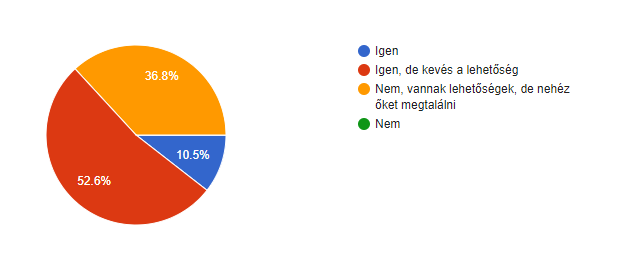
\includegraphics[width=0.8\textwidth]{./images/Screenshot 2024-04-12 165315.png}
    \caption{Könnyen talál sportolási lehetőségeket?}
    \label{fig:do_you_find_options_to_sport}
  \end{figure}

  A választ adók 100\%-ban egyetértettek abban, hogy hasznukra lenne egy olyan webalkalmazás, amely közelebb vinné őket a sportolási lehetőségekhez, 
  és elérhetővé tenné ezeket számukra, továbbá abban is teljes egyetértés volt, hogy nem ismernek más olyan alkalmazásokat,
  amely hasonló szolgáltatást nyújtana számukra.

  A felmérés arra is rámutatott, hogy az emberek azon része, akik szoktak sporteseményeket szervezni, az esetek nagyrészében 
  olyan felületet használnak, amely nem kifejezetten erre a célra készült. Legnépszerűbb megoldások közé tartozik a
  Facebook Messenger, WhatsApp, illetve más chat alapú alkalmazások használata. Ez egy egyszerű és gyors megoldás lehet, viszont 
  könnyen elveszhetnek az információk, és a szervezőknek nehéz lehet a résztvevőkkel való kommunikáció.

  A felmérésből levonható az, hogy a Cronotus projekt egy igényelt webalkalmazás, amely sok ember számára megoldást jelenthet
  a sportolással kapcsolatos nehézségekre nézve, így hozzájárulva a közösség szellemi és fizikai egészségéhez egyaránt.

\section{A Cronotus funkcionalitásai}

A Cronotus webalkalmazása a következő funkcionalításokat kínálja a felhasználó számára:

\begin{itemize}
  \item Regisztráció
  \item Bejelentkezés
  \item Felhasználói adatok listázása
  \item Felhasználói adatok szerkesztése
  \item Felhasználói profilkép és borítókép feltöltése, törlése
  \item Létrehozott sportesemények listázása
  \item Létrehozott sporteseményekre való jelentkezés, leiratkozás
  \item Saját sportesemény létrehozása előre definiált sportok alapján
  \item Saját sporteseményekhez való képek feltöltése, törlése
  \item Sportesemények törlése
\end{itemize}

\section{Szerepkörök}

  A Cronotus két fő szerepkör elkülönítésével közelíti meg a tárgyalt problémát. Az egyik az ``Organizer'', azaz szervezői, a másik pedig
  a ``Player'', avagy játékos szerepkör formájában mutatkozik meg. Egy új felhasználó regisztrálásakor automatikusan mindkét szerepkör
  jóváíródik a felhasználóhoz, így a webalkalmazás lehetőséget nyújt arra, hogy első perctől könnyedén végezhető legyen minden kívánt tevékenység.

  \subsection{A szervező}

  Ahogyan az a \ref{fig:organizer_role}-as ábrán is látható, a szervező szerepkörnek lehetősége van új sportesemények létrehozására,
  az ide tartozó információk könnyed kezelésére, valamint a résztvevőkkel való kommunikációra.
  Továbbá mindamellett, hogy eseményeket hozhat létre, lehetősége van meglévő eseményekre jelentkezni is, mint bármely más felhasználónak.

  \begin{figure}[ht]
    \centering
    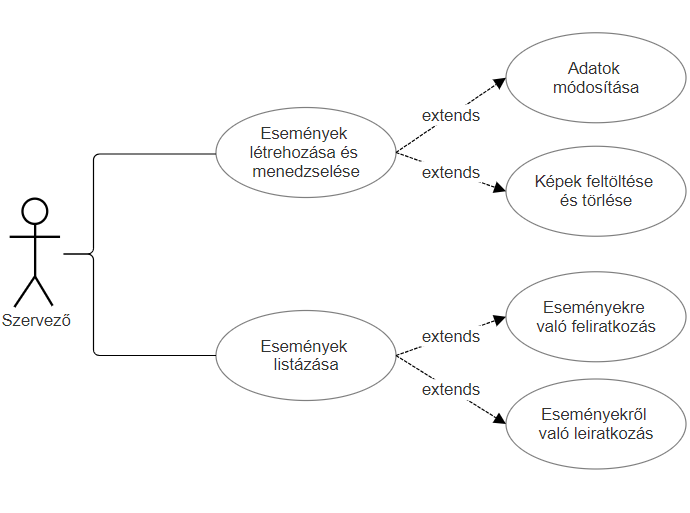
\includegraphics[width=0.8\textwidth]{./images/Screenshot 2024-04-13 021859.png}
    \caption{A szervező szerepkör}
    \label{fig:organizer_role}
  \end{figure}

  \subsection{A játékos}

  Amennyiben egy felhasználó csak arra szeretné használni a felületet, hogy sportolási lehetőségeket találjon, úgy a ``Player'' szerepkör
  lehetőségei tökéletesen elegendőek számára. A játékos felhasználók, a szervezőkhöz hasonlóan listázhatják a már létező eseményeket, 
  jelentkezhetnek ezekre, illetve figyelemmel kísérhetik az eseményekkel kapcsolatos információkat.
  \lstset{style=c_sharp}
  %----------------------------------------------------------------------------
\chapter{Felhasznált technológiák}


A Cronotus alkalmazás két jól elkülöníthető részre bontható fel. Amint a \ref{fig:architecture_overview}-es ábrán is látható, a felhasználói felület weben keresztül érhető el, mely a React\cite{reactdocs} technológia segítségével lett megalkotva TypeScript\cite{typescriptdocs} nyelven, míg az alkalmazás szerver oldali része egy .NET keretrendszeren\cite{dotnetnocs} alapuló program, mely C\# nyelven\cite{csharpdocs} lett megírva és az Entity Framework Core\cite{entityframeworkdocs} által lefektetett szabályrendszert használva kommunikál egy Microsoft SQL Server\cite{sqlserverdocs} adatbázissal, ahol minden adat eltárolásra kerül.
Ahhoz, hogy ezeket az adatokat a felhasználó elérhesse, a kliens és szerver oldal között egy REST API\cite{restfuldocs} segítségével történik meg a kommunikáció.

\begin{figure}[h]
    \centering
    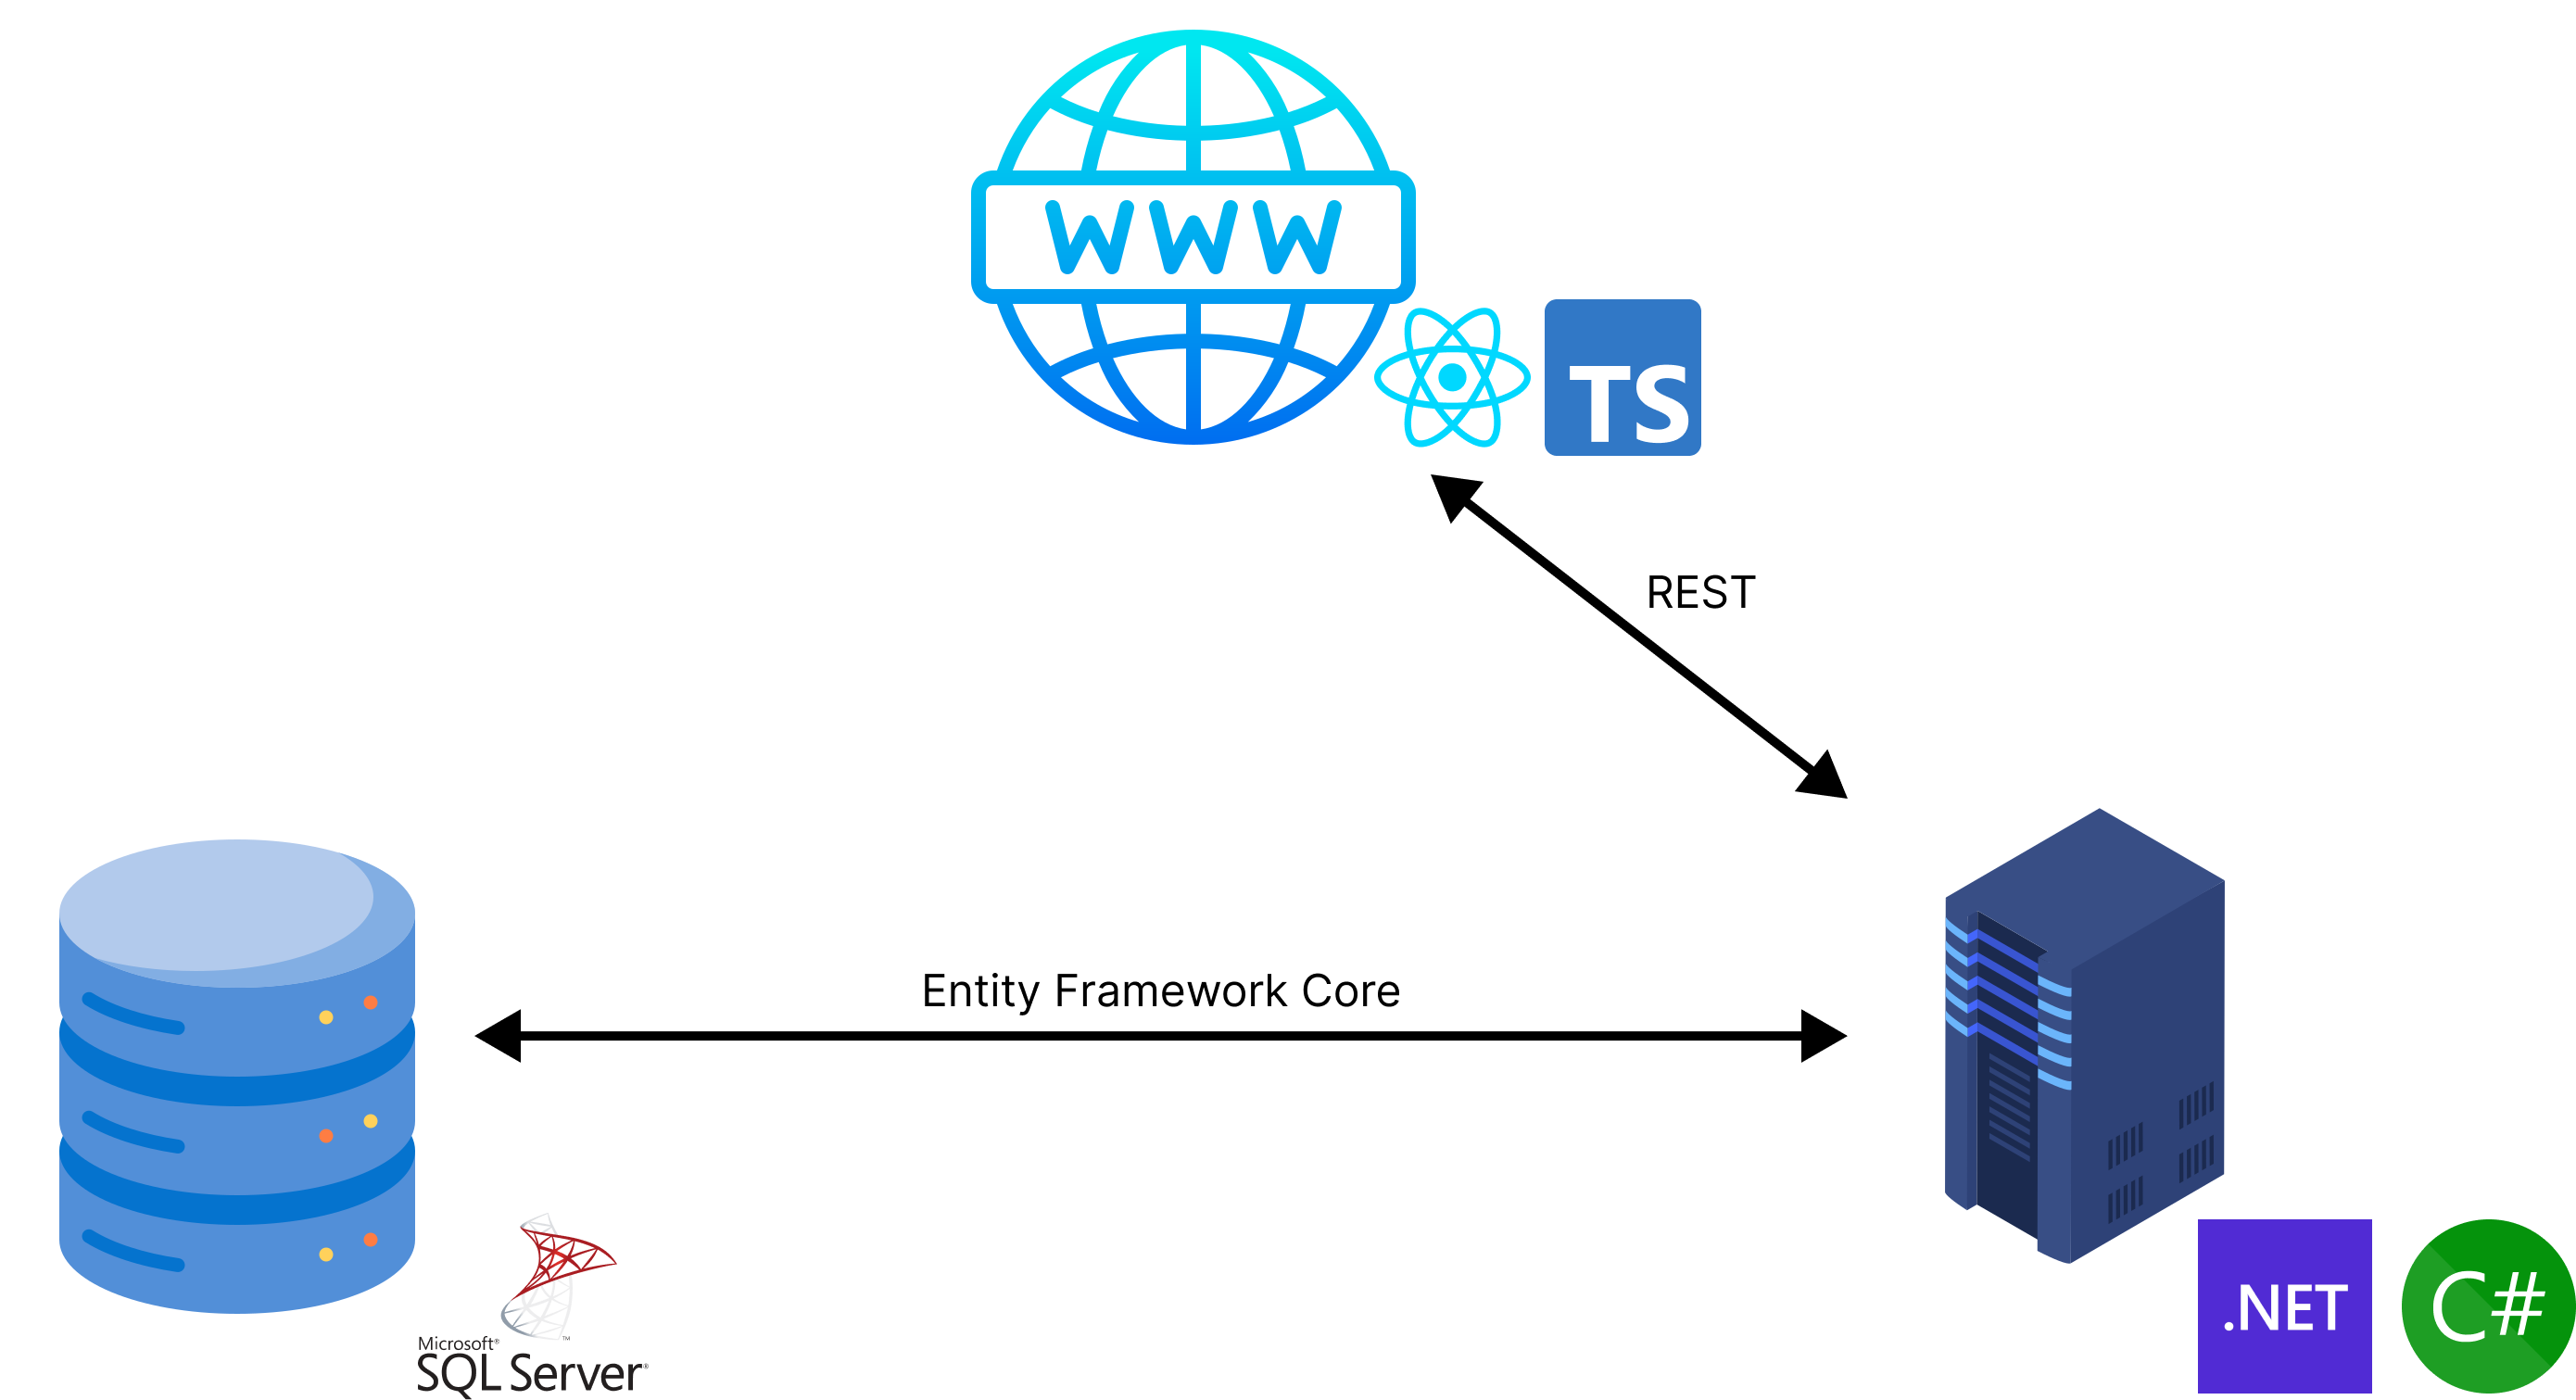
\includegraphics[width=0.8\textwidth]{./images/cronotus_architecture_overview.png}
    \caption{Rendszer architektúra komponensekre bontva}
    \label{fig:architecture_overview}
\end{figure}

%----------------------------------------------------------------------------

%----------------------------------------------------------------------------
\section{A szerver}

A szerver feladata az, hogy kiszolgálja a webalkalmazásról beérkező kéréseket. Ez a feladat alapszinten viszonylag könnyen elvégezhető lenne, viszont nem elég csak csupán elvégezni, hanem a legmegfelelőbb módon kell ezt véghez vinni. Fontos szem előtt tartani a biztonságot, kérésenkénti időt, illetve megbízhatóságot. Az első fontos döntés a szerverrel kapcsolatban az, hogy milyen architekturát valósít meg. A Cronotus esetében egy rétegelt architekturáról\cite{onionarchitecturedocs} beszélhetünk, mely három fő elemre bontja a szerver működését.

\begin{figure}[h]
    \centering
    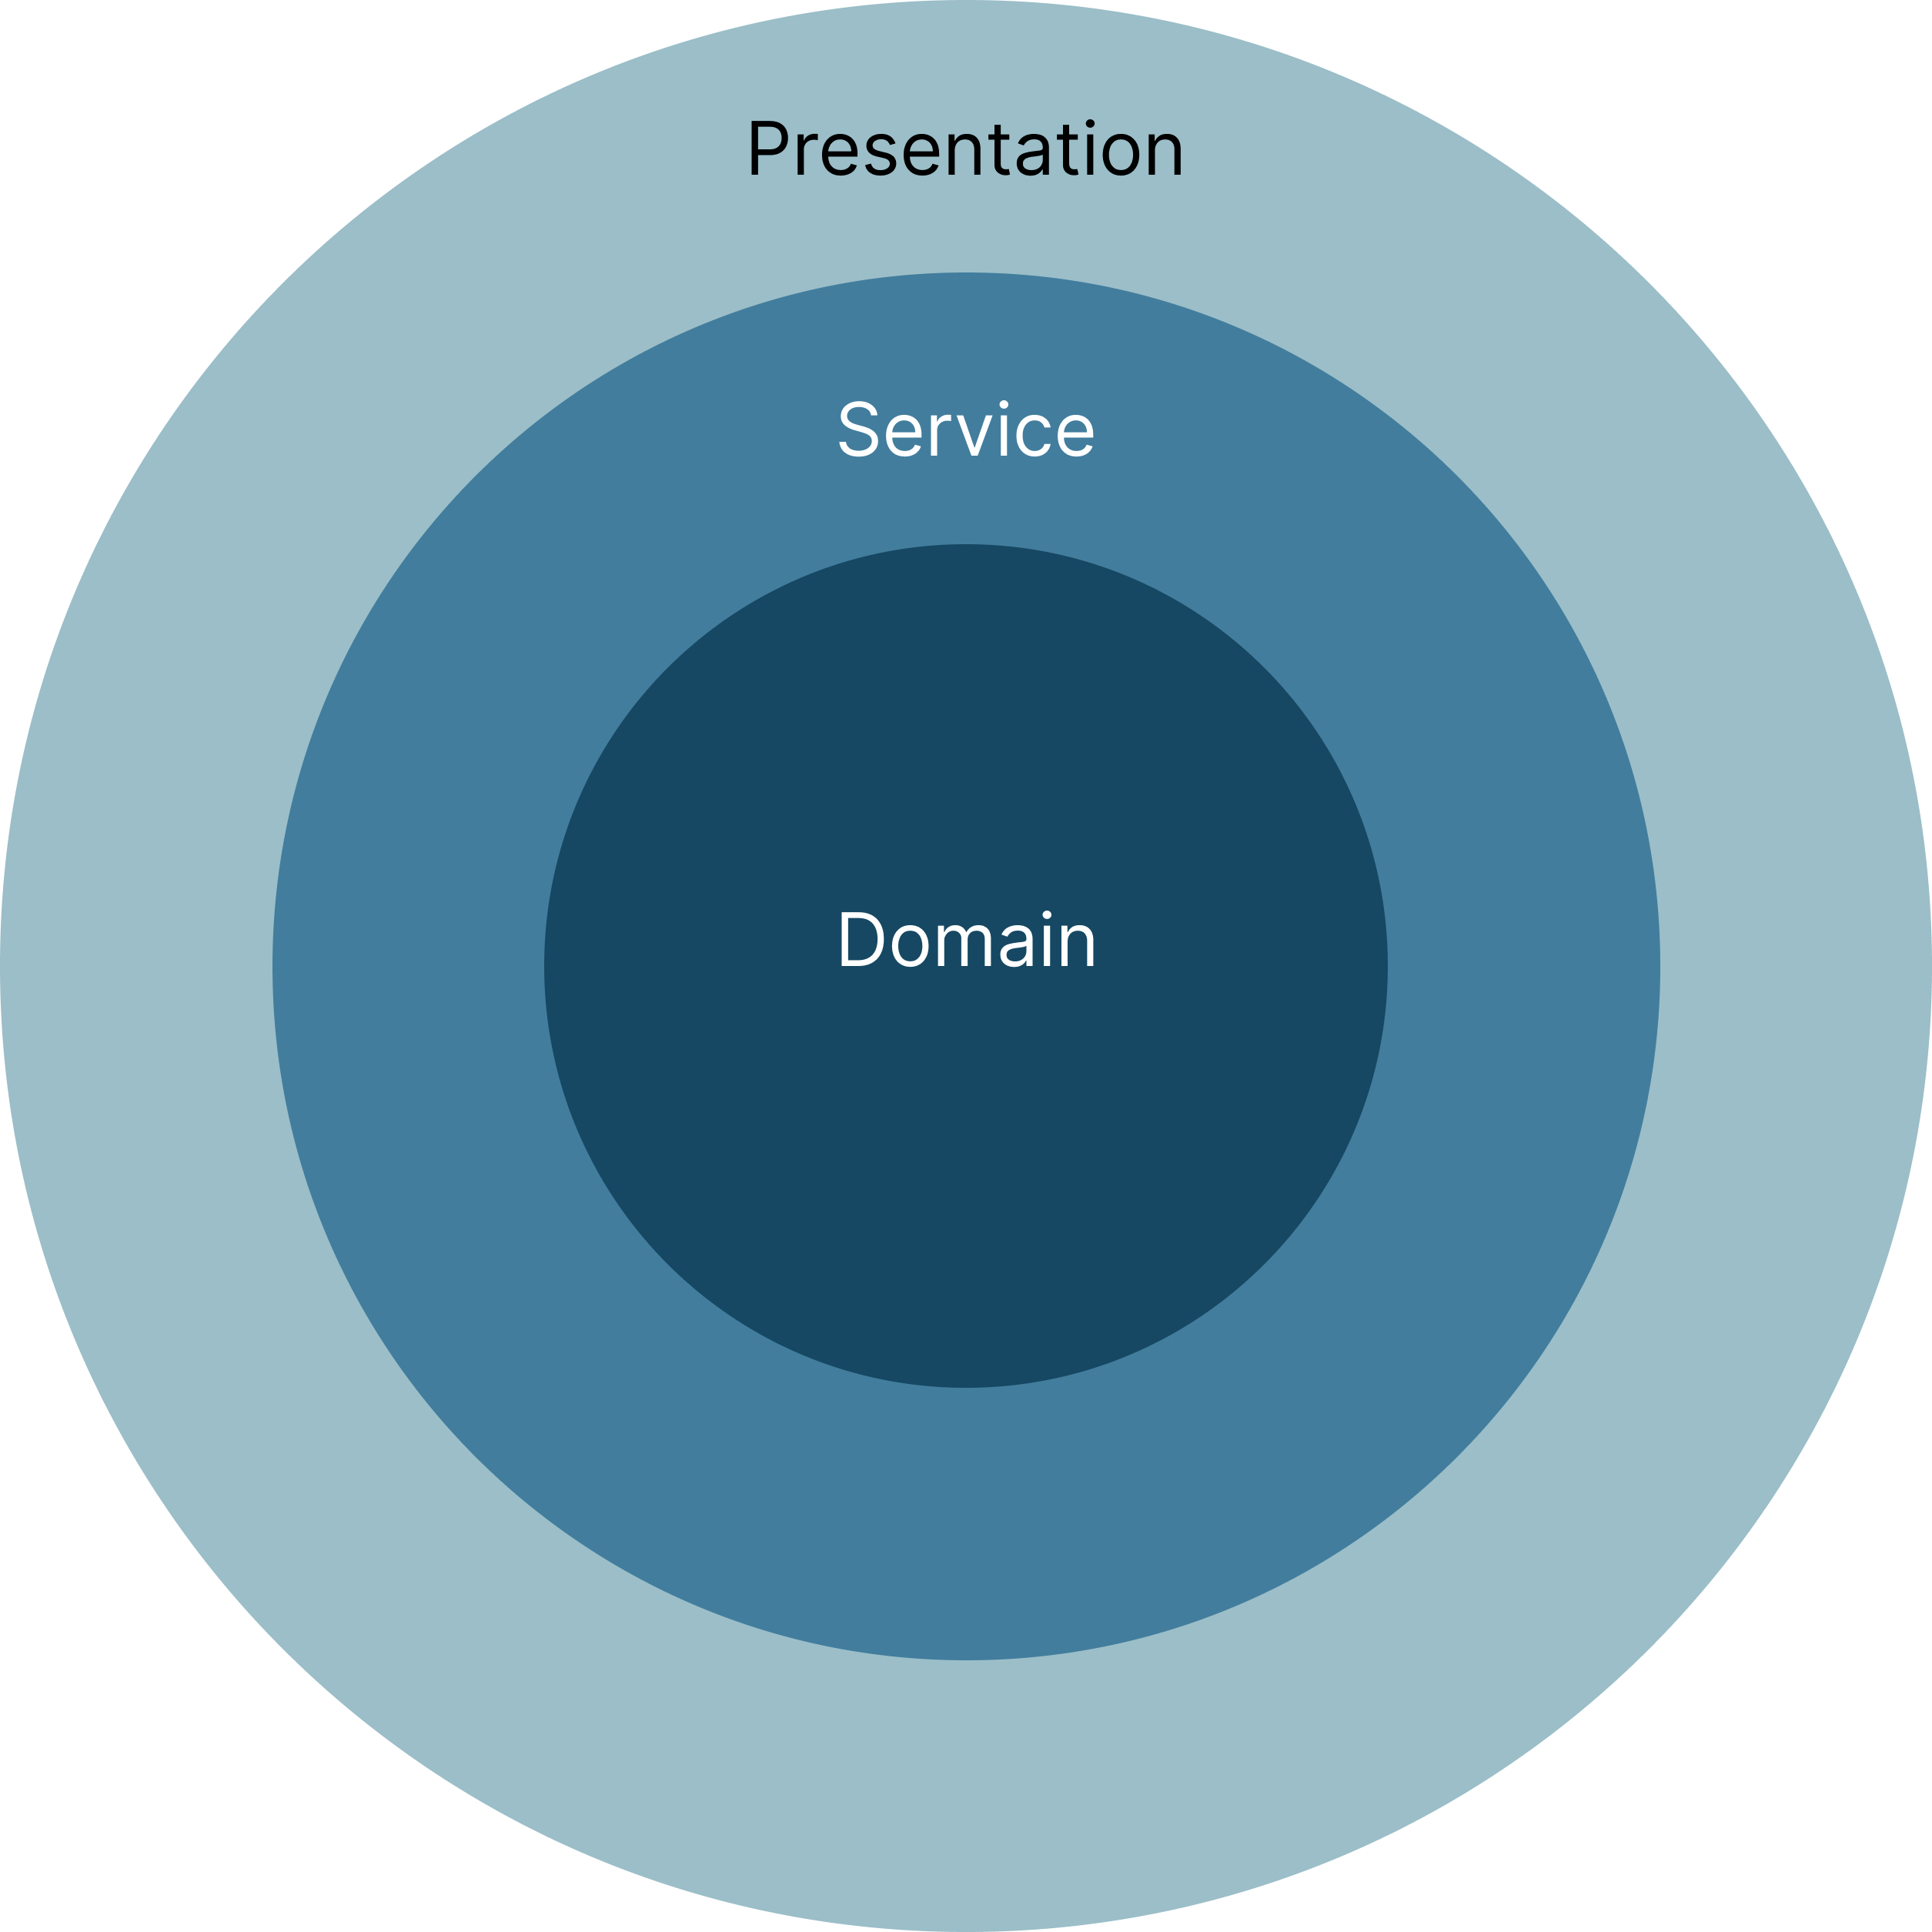
\includegraphics[width=0.6\textwidth]{./images/backend_onion_architecture.png}
    \caption{A rétegelt szerver architektúrája}
    \label{fig:server_onion_architecture}
\end{figure}

A három réteg a \ref{fig:server_onion_architecture}-es ábrán feltüntetett módon helyezkedik el. A legalsó szint a Domain, melynek mindössze annyi a feladata, hogy az adatbázissal kommunikáljon. Ezen a szinten történik meg az adatok kinyerése, vagy akár az alapszintű műveletek véghezvitele, például létrehozás, vagy törlés.

A kör középpontjától kifele haladva a következő a Service réteg. Ez az a szint, amely a biznisz logikát végrehajta a kapott adatokon. Abban az esetben, ha a kliens oldal egy kérést küld valameny adat lekérésére, úgy a kéréshez szükséges eredmény ezen a szinten formálódik olyan alakba, amely megfelelő a fogyasztónak. A szint felelősége úgy is felfogható, mint egy tolmács, mely a kliens és Domain között működik. Főbb feladatai a komplex struktúrájú adatok egyszerű alakra és utasításokra bontása, illetve egyszerű adatok előkészítése és prezentálható formába szervezése a kliens számára.

A legfelső, a Presentation réteg feladata a fogyasztó irányába történő kérésekkel kapcsolatos visszajelzések megfelelő kezelése, illetve a Service rétegtől kapott adatok átirányítása a helyes HTTP kóddal.

\subsection{A rétegelt architektúra előnyei}

Felmerülhet a kérdés, hogy miért érdemes az előbbiekben [\ref{fig:server_onion_architecture}] bemutatott formába szervezni a szerver felépítését. 
Ahhoz, hogy ezt bemutassuk, fontos először megvizsgálni az architektúrán belüli egyes rétegek közti függőségek folyását. 
Ha ezt a felépítést követjük, akkor a függőségek a legbelső szintektől a felsőbb szintek irányába folynak, azaz a Domain réteg nem függ semmítől. 
Ez betudható szabályként is, tehát egy réteg minél alacsonyabban van a felépítésben, annál kevesebb függősége van.
Az előbbiekben leírt függőségi irányzat úgy is nevezhető, mint az úgynevezett Inversion of Control (IoC) \cite{inversionofcontroldocs}.

Továbbá minden réteg csakis kizárólag az alatta levő rétegre hivatkozhat. Ez azért hasznos, mert így nem kall aggódnunk afelől, hogy hogyan fog egy felsőbb szintű művelet implementálni egy alacsonyabb osztályút, elég kontraktokat felállítanunk, melyeket teljesíthetnek a felső rétegek. Ez fontos tulajdonsága az architektúrának, hiszen nagy szabadságot nyújt egyes szintek elkészítésében, hiszen elég csak az oda tartozó logikára figyelnünk.

\begin{figure}[h]
    \centering
    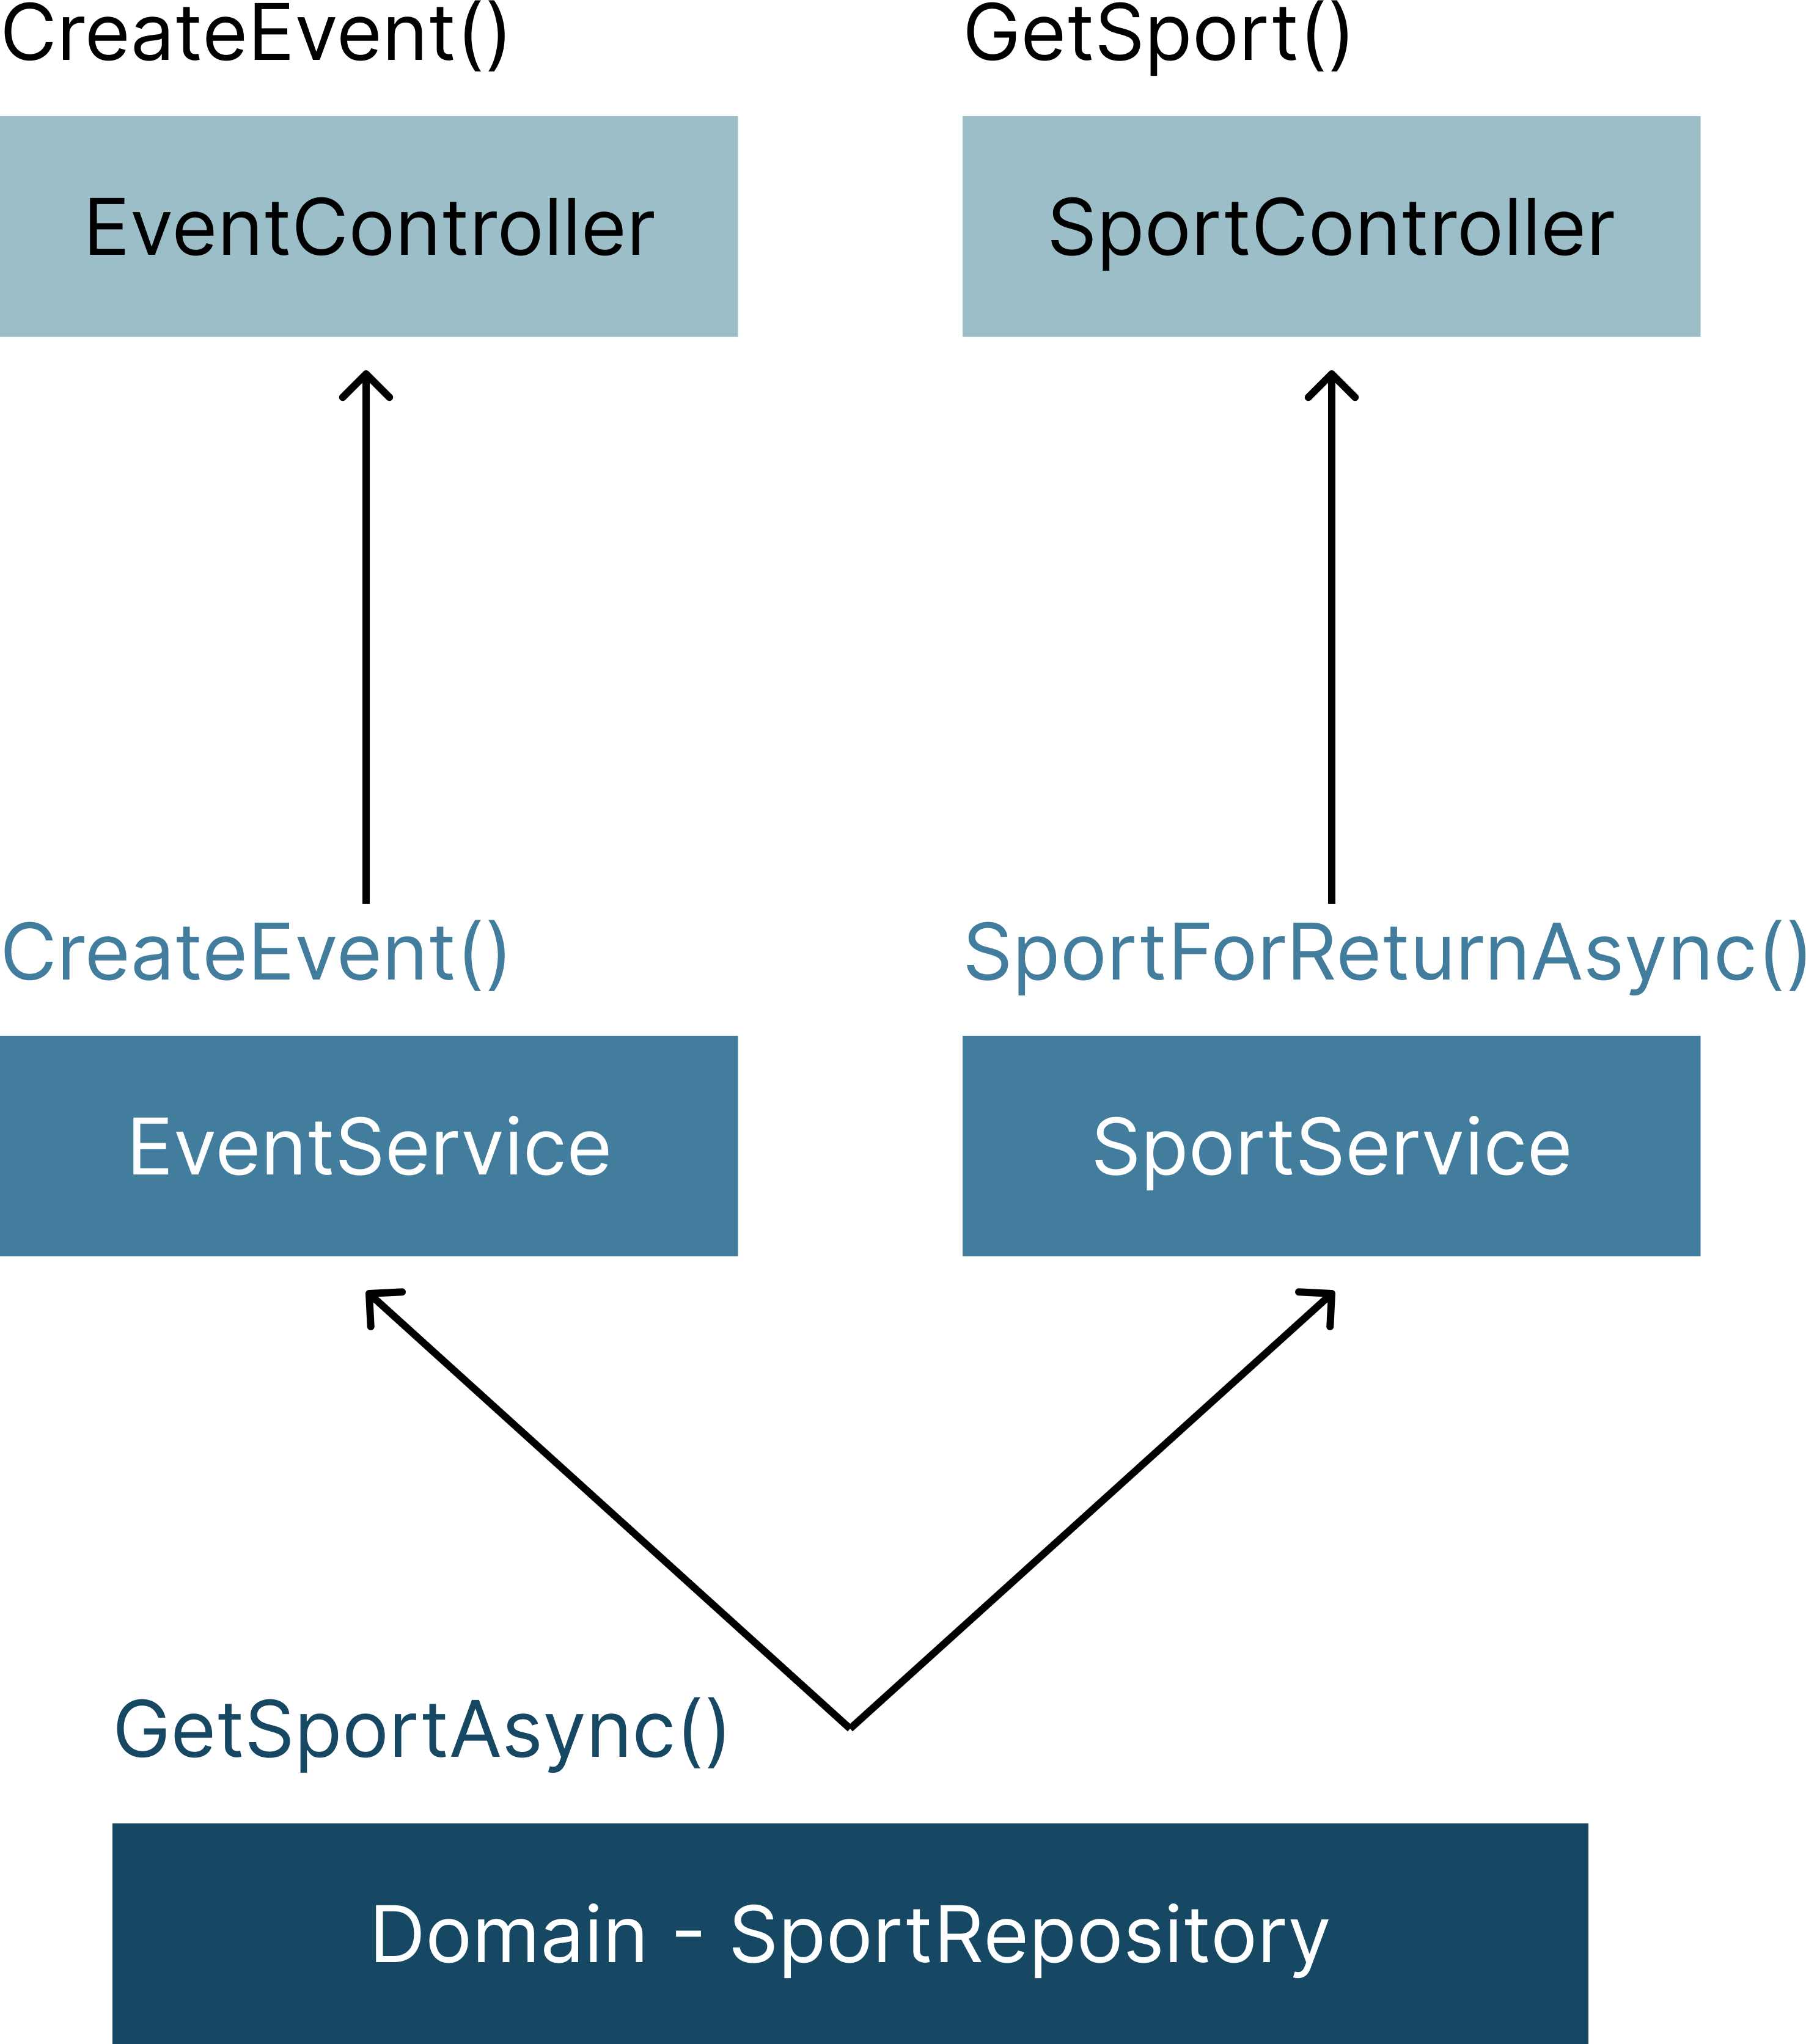
\includegraphics[width=0.6\textwidth]{./images/get_sport_example.png}
    \caption{A SportRepository egy Domain szintű műveletének eredményének kétféleképpen való felhasználása felsőbb szinteken}
    \label{fig:sport_repo_usage_example}
\end{figure}

A \ref{fig:sport_repo_usage_example}-as ábrán látható egy példa, mely a rétegelt architektúra egy előnyét használja fel. A SportRepository-ban rendelkezésünkre áll egy függvény, mely egy Sport Entity-t térít vissza. A Repository-nak ebben az esetben nem kell tudnia, hogy hogyan fogják a felsőbbrendű rétegek felhasználni az innen kapott adatot. Az EventService arra használja fel az adatot, hogy ellenőrzés alá vesse a létrehozandó eseményhez kiválasztott sportot, vajon létezik-e? A SportService viszont arra használja fel ugyanazt az eredményt, hogy egy prezentálható formában vissza térítse a Presentation szintnek a sportot, ami egy Controller formájában elérhetővé teszi a kliens számára, hogy lekérhessen egy sportot ID alapján.

\subsection{Az adatbázis}

A rendszer adatai egy Microsoft SQL Server relációs adatbázisban\cite{relationaldatabasedocs} vannak eltárolva. Mivel a rendszer személyes információkat tárol el a felhasználóiról, szükséges volt egy olyan adatbázist választani, mely megfelelő képpen tudja kezelni az egyes felhasználók és felhasználókhoz kötődő entitások közötti kapcsolatokat. Továbbá az is fontos, hogy biztonságosan legyenek az adatok tárolva. Mindezeket  figyelembe véve egy relációs adatbázis volt a legjobb választás. A konkrét döntés azért esett a Microsoft SQL Server termékre, mivel a szerver fő keretrendszere alapból Microsoft termék, így a Microsoft-készített adatbázis egy jó integrálhatósági lehetőségnek bizonyul. Továbbá a technológiák megegyezése elősegít a későbbi felhőbe való kitelpítésben is.

Az adatbázis strukturális létrehozása a \textit{code first approach}\cite{codefirstapproachdocs} elv segítségével hajtódik végre, ahogyan a \ref{fig:code_first_approach}-es ábrán is látható. Az Entity Framework Core lehetővé teszi azt, hogy adatmodellek és adatmodellek közti kapcsolatok alapján migrációk segítségével változtassunk az adatbázis sémán, illetve az abba tartozó adatokon.

\begin{figure}[h]
    \centering
    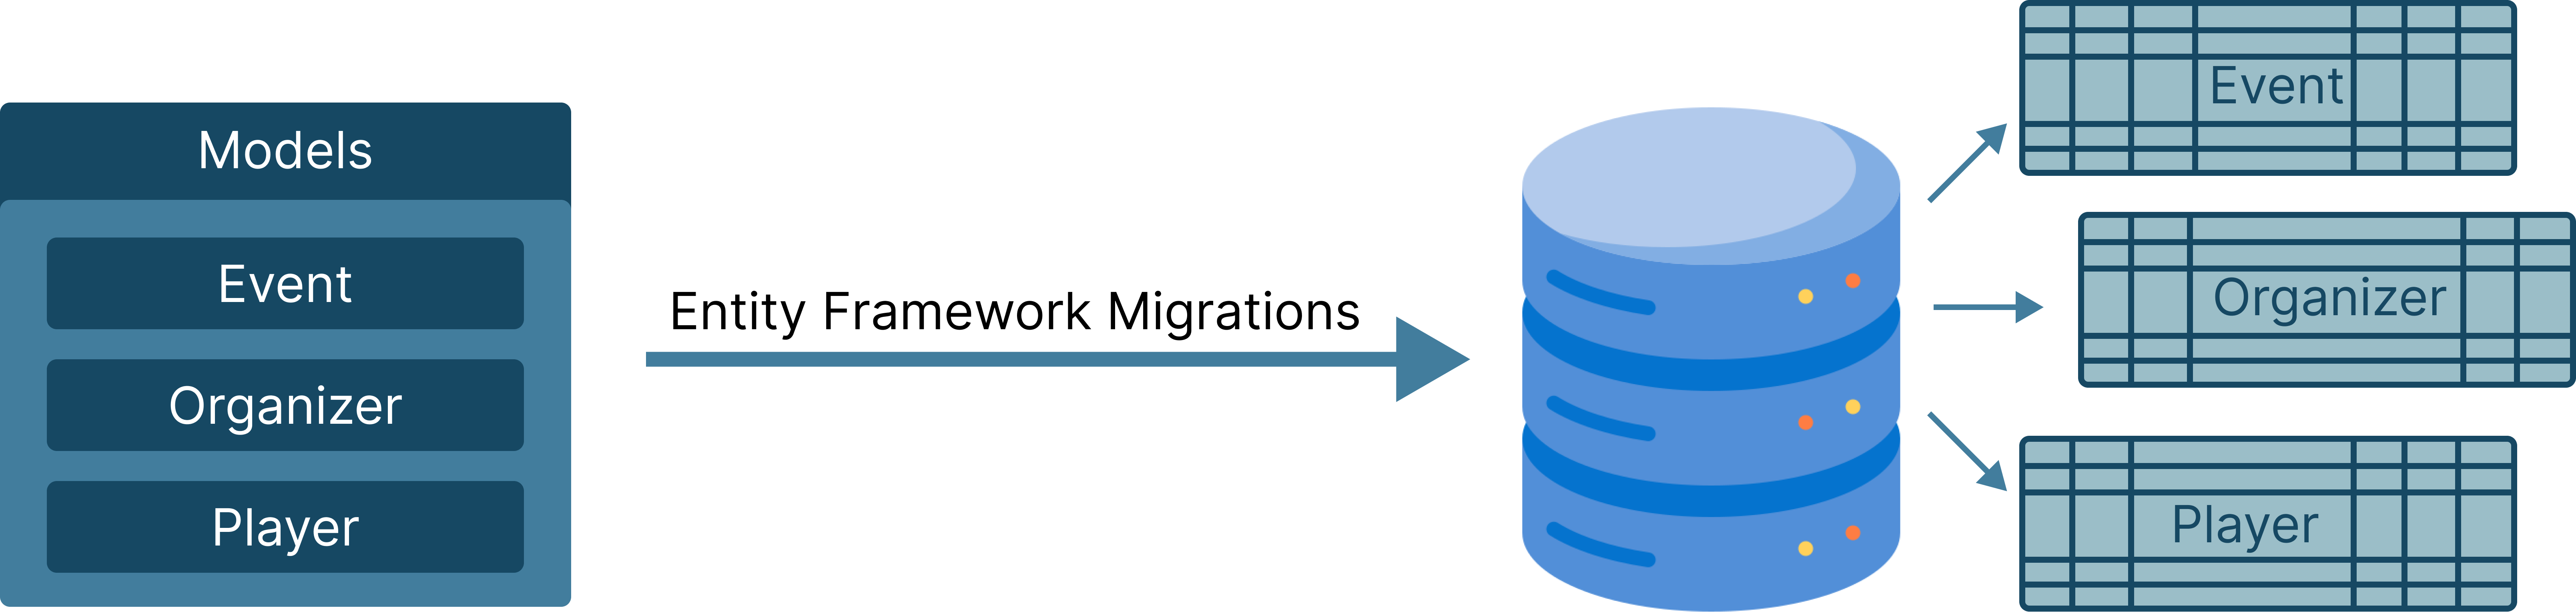
\includegraphics[width=\textwidth]{./images/code_first_approach.png}
    \caption{A Code First Approach áttekintése}
    \label{fig:code_first_approach}
\end{figure}

Technikailag megvizsgálva, a Code First Approach [\ref{fig:code_first_approach}-es ábra] az Entity Framework Core egyik hozománya, mely az ORM (Object Relational Mapper)\cite{codefirstapproachdocs} segítségével képes a \textit{DbContext} osztályon keresztül kapcsolatba lépni az adatbázissal, továbbá a \textit{RepositoryBase} absztrakt osztályon végrehatjtandó CRUD műveletek\cite{crudoperationdocs} segítségével tudja az itt tárolt entitásokat kezelni, törölni vagy újakat létrehozni.

\subsection{A Cronotus API}

A kliens oldali kéréseket a szerver a Presentation [\ref{fig:architecture_overview}-es ábra] rétege fogadja és szolgálja ki. A \textit{pipeline}-ja HTTPS (HyperText Transfer Protocol Secure)\cite{httpsdocs} protokolt követve üzemel. A kliens HTTP kéréseket küldve tud adatokat küldeni, lekérni, illetve szerveri erőforrásokat igénybe venni adatokkal kapcsolatos műveletekhez. Az adatokat DTO-k (Data Transfer Object)\cite{dtodocsmicrosoft} formájában cserélgeti a kliens a szerver oldallal, mely JSON (JavaScript Object Notation)\cite{jsondocs} formájában valósul meg. 

A szerver minden beérkező kérést átfuttat egy ellenőrzésrendszeren [\ref{fig:pipeline}-ös ábra], mely az Application Pipeline formájában van felépítve. Itt biztonsági és adatintegritási szempontból fontos vizsgálat alá veti a kéréseket. A szerver a pipeline-ban érvényesíti azt, hogy HTTP helyett biztosan HTTPS protokllon keresztül történjen meg a kommunikáció, hiszen így egy harmadik fél nem tudja leolvasni a küldött kérések tartalmát, úgy sem ha hozzáférése van ezekhez, mivel kódolva vannak. A pipeline továbbá más hasznos beállításokat is érvényesít, például azt, hogy csak megfelelő URL címekről legyen engedélyezett a hozzáférés a szerverhez, illetve jogosultságot vizsgál \textit{Authentication} és \textit{Authorization}\cite{authflowsdocs} segítségével.

\begin{figure}[h]
    \centering
    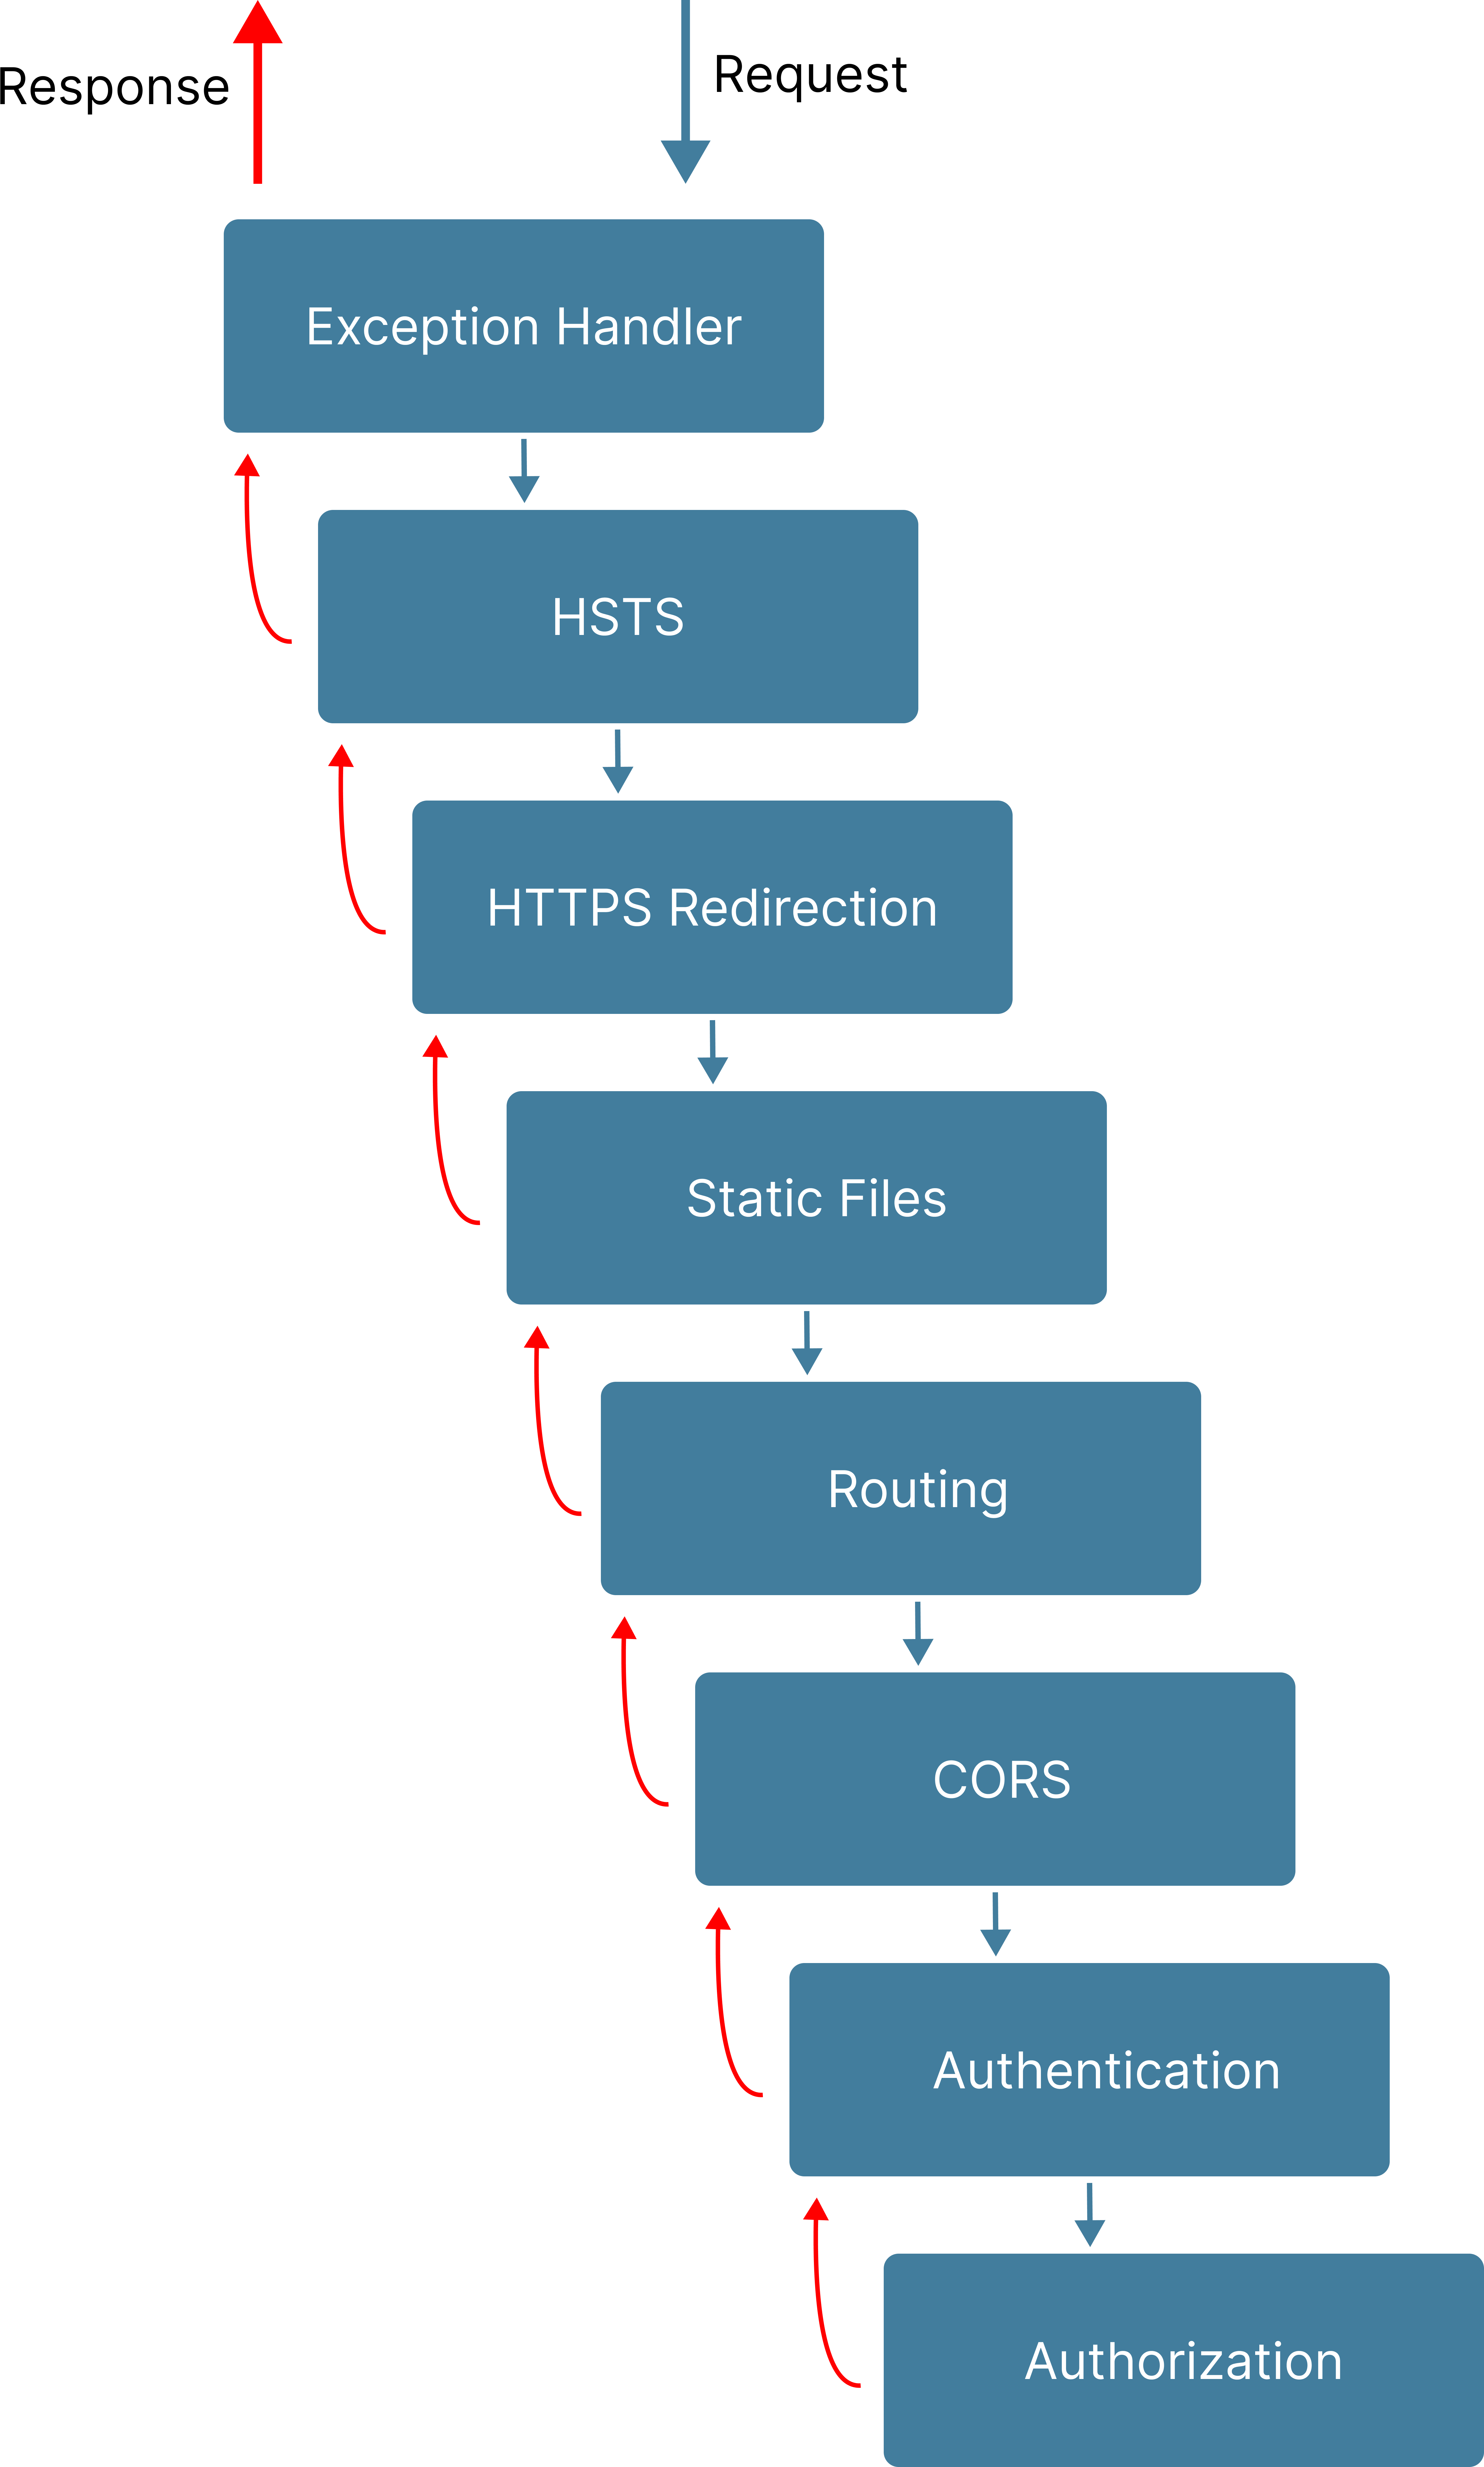
\includegraphics[width=0.6\textwidth]{./images/pipeline.png}
    \caption{A pipeline, melyen keresztül kell mennie minden szerver fele érkező kérésnek}
    \label{fig:pipeline}
\end{figure}

\subsection{Hitelesítés és Engedélyezés}

Az rendszer JWT Tokenek\cite{jwtdocs} formájában kezeli a felhasználói munkamenetet és az ezekbe kódolt információk segítségével végzi el a felhasználók hitelesítését és bírálja el az \textit{endpoint}-okhoz való hozzáférésüket.

Egy ilyen token fontos információkat tartalmaz, például felhasználói jogok, jogokhoz kapcsolódó id-k, illetve a token lejárati dátuma. 

A kliens oldalról kapott kérések mindegyikéhez csatolva van egy ilyen JWT token, amit a rendszer egy kérés beérkeztekor dekódol, majd az innen kinyert információk segítségével megnézi, hogy érvényes-e a token, majd ellenőrzi, hogy a felhasználónak van-e joga végrehajtani a kívánt műveletet. Egy token élettartama 10 perc, ezután egy \textit{Refresh Token} segítségével a kliens újat kell kérjen. Ez a fajta viszonylag rövid szsavatossági idő egy fontos biztonsági intézkedés, mivel ha egy harmadik fél meg is tud szerezni egy ilyen érvényes tokent, akkor is csak maximum 10 perce van arra, hogy hozzáférése legyen a szerverhez. 

\subsection{Globális hibakezelés}

Annak érdekében, hogy a kód átlátható és könnyen karbantartható legyen a hiba és kivételkezelést a projekt egy globális hibakezelő middlware segítéségvel oldja meg, mely részét képezi az application pipeline-nak.

Ha ezt a kezelési módszert használjuk, akkor nincs szükség \textit{try - catch} kódblokkok használatára, hiszen ha valamilyen kivétel merül fel, akkor azt elég csak tovább dobni, majd a middleware automatikusan lekezeli. A kezelés során a middleware beállítja a visszatérítendő objektumba a fellépő hiba HTTP státuszkódját, majd a kiindulási pontból dobott hiba üzenetét, mindezt annak érdekében, hogy kliens oldalon könnyen olvasható legyen, hogy egyes hiba miből származhat.

%----------------------------------------------------------------------------
%----------------------------------------------------------------------------
\section{A felhasználói felület}

A felhasználói felület egy webalkalmazás formájában nyilvánul meg. A felhasználók itt végezhetnek eseményekkel kapcsolatos műveleteket, például létrehozás, csatlakozás, vagy kommentelés. Ez az alfejezet a felhasználói felület felépítését és működését tárgyalja.

\subsection{Felhasznált technológia}

A webalkalmazás TypeScript\cite{typescriptdocs} nyelven íródott, React\cite{reactdocs} könyvtár felhasználásával.
A TypesScript a JavaScript\cite{javascriptdocsmozilla} nyelvet bővíti ki egy szintaxis csomaggal, amely lehetővé teszi a változók és objektumok típuskezelését, ezzel egy jobban átlátható és biztonságosabb fejlesztési procedúrát nyújtva.

A React könyvtár segítségével a webalkalmazás egy Single Page Application (SPA)-ként\cite{singlepageapplicationdocs} működik.
A SPA az egész weboldalt egyetlen HTML dokumentumban építi fel, majd változás során ennek a tartalmát frissíti és cseréli. Ez előnyös megoldás, mivel így nem kell minden oldalcsere, illetve tartalomfrissítés után újratölteni az alkalmazást, így gyorsabb lesz, javítja a felhasználói élményt.

Az alkalmazáshoz felhasznált további könyvtárcsomagok kezelése, a webalkalmazás futtatása, illetve építése a Vite\cite{vitedocs} segítségével van megoldva.
A Vite egy gyors és egyszerű build eszköz, mely alkalmas React webalkalmazások kezelésére. Lehetővé tesz Live Reloading-ot mely hasznos a fejlesztés során, illetve úgy van felépítve, hogy minimalizálja az alkalmazás építéséhez szükséges időt, így mégjobban gyorsítva és javítva a fejlesztési időt, élményt.

Az alkalmazás felhasználói felületének egy szerves része továbbá a React könyvtárra épített Material UI komponens csomag, mely segítségével könnyen és gyorsan lehet előre megépített megjelenítő komponenseket felhasználni.

\subsection{Kommunikáció a szerverrel}

A webalkalmazás HTTPS protokollon keresztül kommunikál a szerverrel. A HTTPS protokoll a HTTP protokoll biztonságos formája. Itt a HTTP-vel ellentétben az adatok nem egyszerű szöveges formátumban vannak küldve, hanem kódolt blokkokként, melyek biztosítják azt, hogy út közben egy rosszindulatú harmadik félnek ne legyen hozzáférése bármilyen kommunikációhoz.

Az alkalmazás GET metódusokra az SWR - Data Fetching\cite{swrdocs} könyvtárcsomagot használja. Az SWR rövidítés az angol ``stale-while-revaildate'' szókapcsolatoban ered, mely annyit tesz, hogy ``elavult-közben-újraérvényesít''. Az SWR adatlekérési stratégia alapján egy kérés után előszőr a potenciális elavult adatot megkapjuk egy cache (stale) tároló rendszerből, majd elküldjük a kérést a legfrissebb adatért (revalidate), majd végül előállunk ezzel.

A könyvtárcsomag lehetőséget biztosít arra is, hogy az adatlekéréssel kapcsolatos státuszokat kezeljük, például kérés alatt töltés ideje, illetve hibákat. Ezt egyszerűen megtehetjük a függvényhívás esetén, amint a \ref{lst:typescript_example}-es kódrészleten is látszik.

\begin{lstlisting}[caption={SWR használata profil adatok lekérésére}, label={lst:typescript_example}]
const { data: profileInfo, isLoading, error, mutate } = useProfile(userId!);

{isLoading ? (
            <ProfileTitleIsLoading />
          ) : (
            <ProfileHead
              profileInformation={profileInfo!}
              className="profile-head"
            />
          )}
\end{lstlisting}

A \ref{lst:typescript_example}-es ábrán látható, hogy abban az esetben, ha az adatok még lekérés alatt vannak, a komponens a ``ProfileTitleIsLoading'' komponenset tölti be, majd amint a a betöltés befejeződik, megjeleníti a betöltött adatokat.

Amennyiben a szerverhez intézett HTTP kérés nem GET metódus, úgy az alkalmazás nem SWR-t használ, hanem egy egyszrű, dinamikusan felépített fetchert. Ez a fetcher függvény újrahasznosítható, így elég minden egyedi kérés esetében csak megadni a megfelelő adatokat, endpoint címet, és meghívni az ehhez tartozó fetchert.

A \ref{fig:fetchingData}-os ábra szemlélteti néhány végpont egyszerűsített működését.

\begin{figure}[ht]
  \centering
  \includegraphics[width=\textwidth]{./images/fetchingData.png}
  \caption{Néhány endpoint működése}
  \label{fig:fetchingData}
\end{figure}

\subsection{Oldalak közötti navigálás}

A webalkalmazáson való oldalak közötti navigációért a React Router\cite{reactrouterdocs} könyvtárcsomag felelős. Ez lehetővé teszi azt, hogy könnyen és zökkenőmentesen tudjunk oldalak között navigálni, illetve ennek során információt cserélni egyes oldalak, komponensek között.

A React Router lehetővé teszi azt, hogy deklaráljunk minden létező oldalt egy ``Router'' komponensben, ahonnan aztán a Single Page Application dinamikusan cserélni tudja a pillanatynyilag megjelenített oldalt. Ez a deklarálási módszer látható a \ref{lst:router_component}-as kódrészletben.

\begin{lstlisting}[caption={Route-ok deklarálása}, label={lst:router_component}]
const Router = (props: { onLogout: () => void }) => {
  return (
    <Routes>
      <Route path="/" element={<Layout />}>
        <Route index element={<Home />} />
        <Route path="browser" element={<Browser />} />
        <Route path="create-event" element={<CreateEvent />} />
        <Route path="event/:id" element={<SportsEvent />} />
        <Route path="profile" element={<Profile onLogout={props.onLogout} />} />
        <Route path="*" element={<NoMatch />} />
      </Route>
    </Routes>
  );
};
\end{lstlisting}

Abban az esetben, ha kliens oldalon böngészőn belül nem a megfelelő cím kerül megadásra, úgy a ``NoMatch'' route kerül betöltésre. Ez hasznos, mivel ha a felhasználó egy nem létező oldalt akar betölteni, akkor nem egy érthetetlen hibaüzenet kerül elé, hanem egy általunk felépített érthető visszajelzés.

\subsection{Munkamenetkezelés JWT tokenekkel}

A webalkalmazás biztonságos működését JWT (JSON Web Token)-ek segítik elő. A JWT egy szerkezetileg három részből álló metódusa annak, hogy két fél biztonságosan információt válthasson egymás között. 

A webalkalmazás szintjén ahhoz, hogy a Authentication és Authorization-el kapcsolatos feladatokat elvégezzük ilyen tokeneket használunk. Minden szerverhez intézett kéréshez a HTTP kérés Header részébe egy ilyen token van csatolva, amely segítségével elérhetőek a jogrendszer szerinti védett endpointok. A tokenekbe bele van kódolva a felhasználókhoz kapcsolódó egyedi azonosítók, jogok, illetve a token lejárási ideje.

A lejárási idő a webalkalmazás szintjén fontos, mivel ennek függvényében lehet a munkamenetet követni. Abban az esetben ha egy token lejár, a felhasználó alap esetben arra van kérve, hogy jelentkezzen be újra. Ez azért hasznos, mert ha egy harmadik rosszindulatú fél meg is szerez egy ilyen tokent, csak limitált ideje van kárt tenni a rendszerben, esetünkben 10 perc.

Ahhoz, hogy egy jó felhasználói élményt nyújtson a webalkalmazás, két féle tokent használunk. Van access token, illetve refresh token. Az access tokenek magukba foglalnak minden olyan információt és működési elvet, melyet a fentiekben tárgyaltunk. Azért, hogy egy access token lejártakor ne kelljen újra bejelentkeznie a felhasználóknak, refresh tokeneket használ az alkalmazás, melyek adatbázisban tárolva vannak minden felhasználó számára. Ezek segítségével új access tokent lehet generálni, így nem szükségeltetve az újboli bejelentkezést 10 percenként.

A \ref{fig:jwt_auth_process}-es ábra bemutatja a JWT tokenek segítségével vezetett munkamanetkezelés logikáját.

\begin{figure}[h]
  \centering
  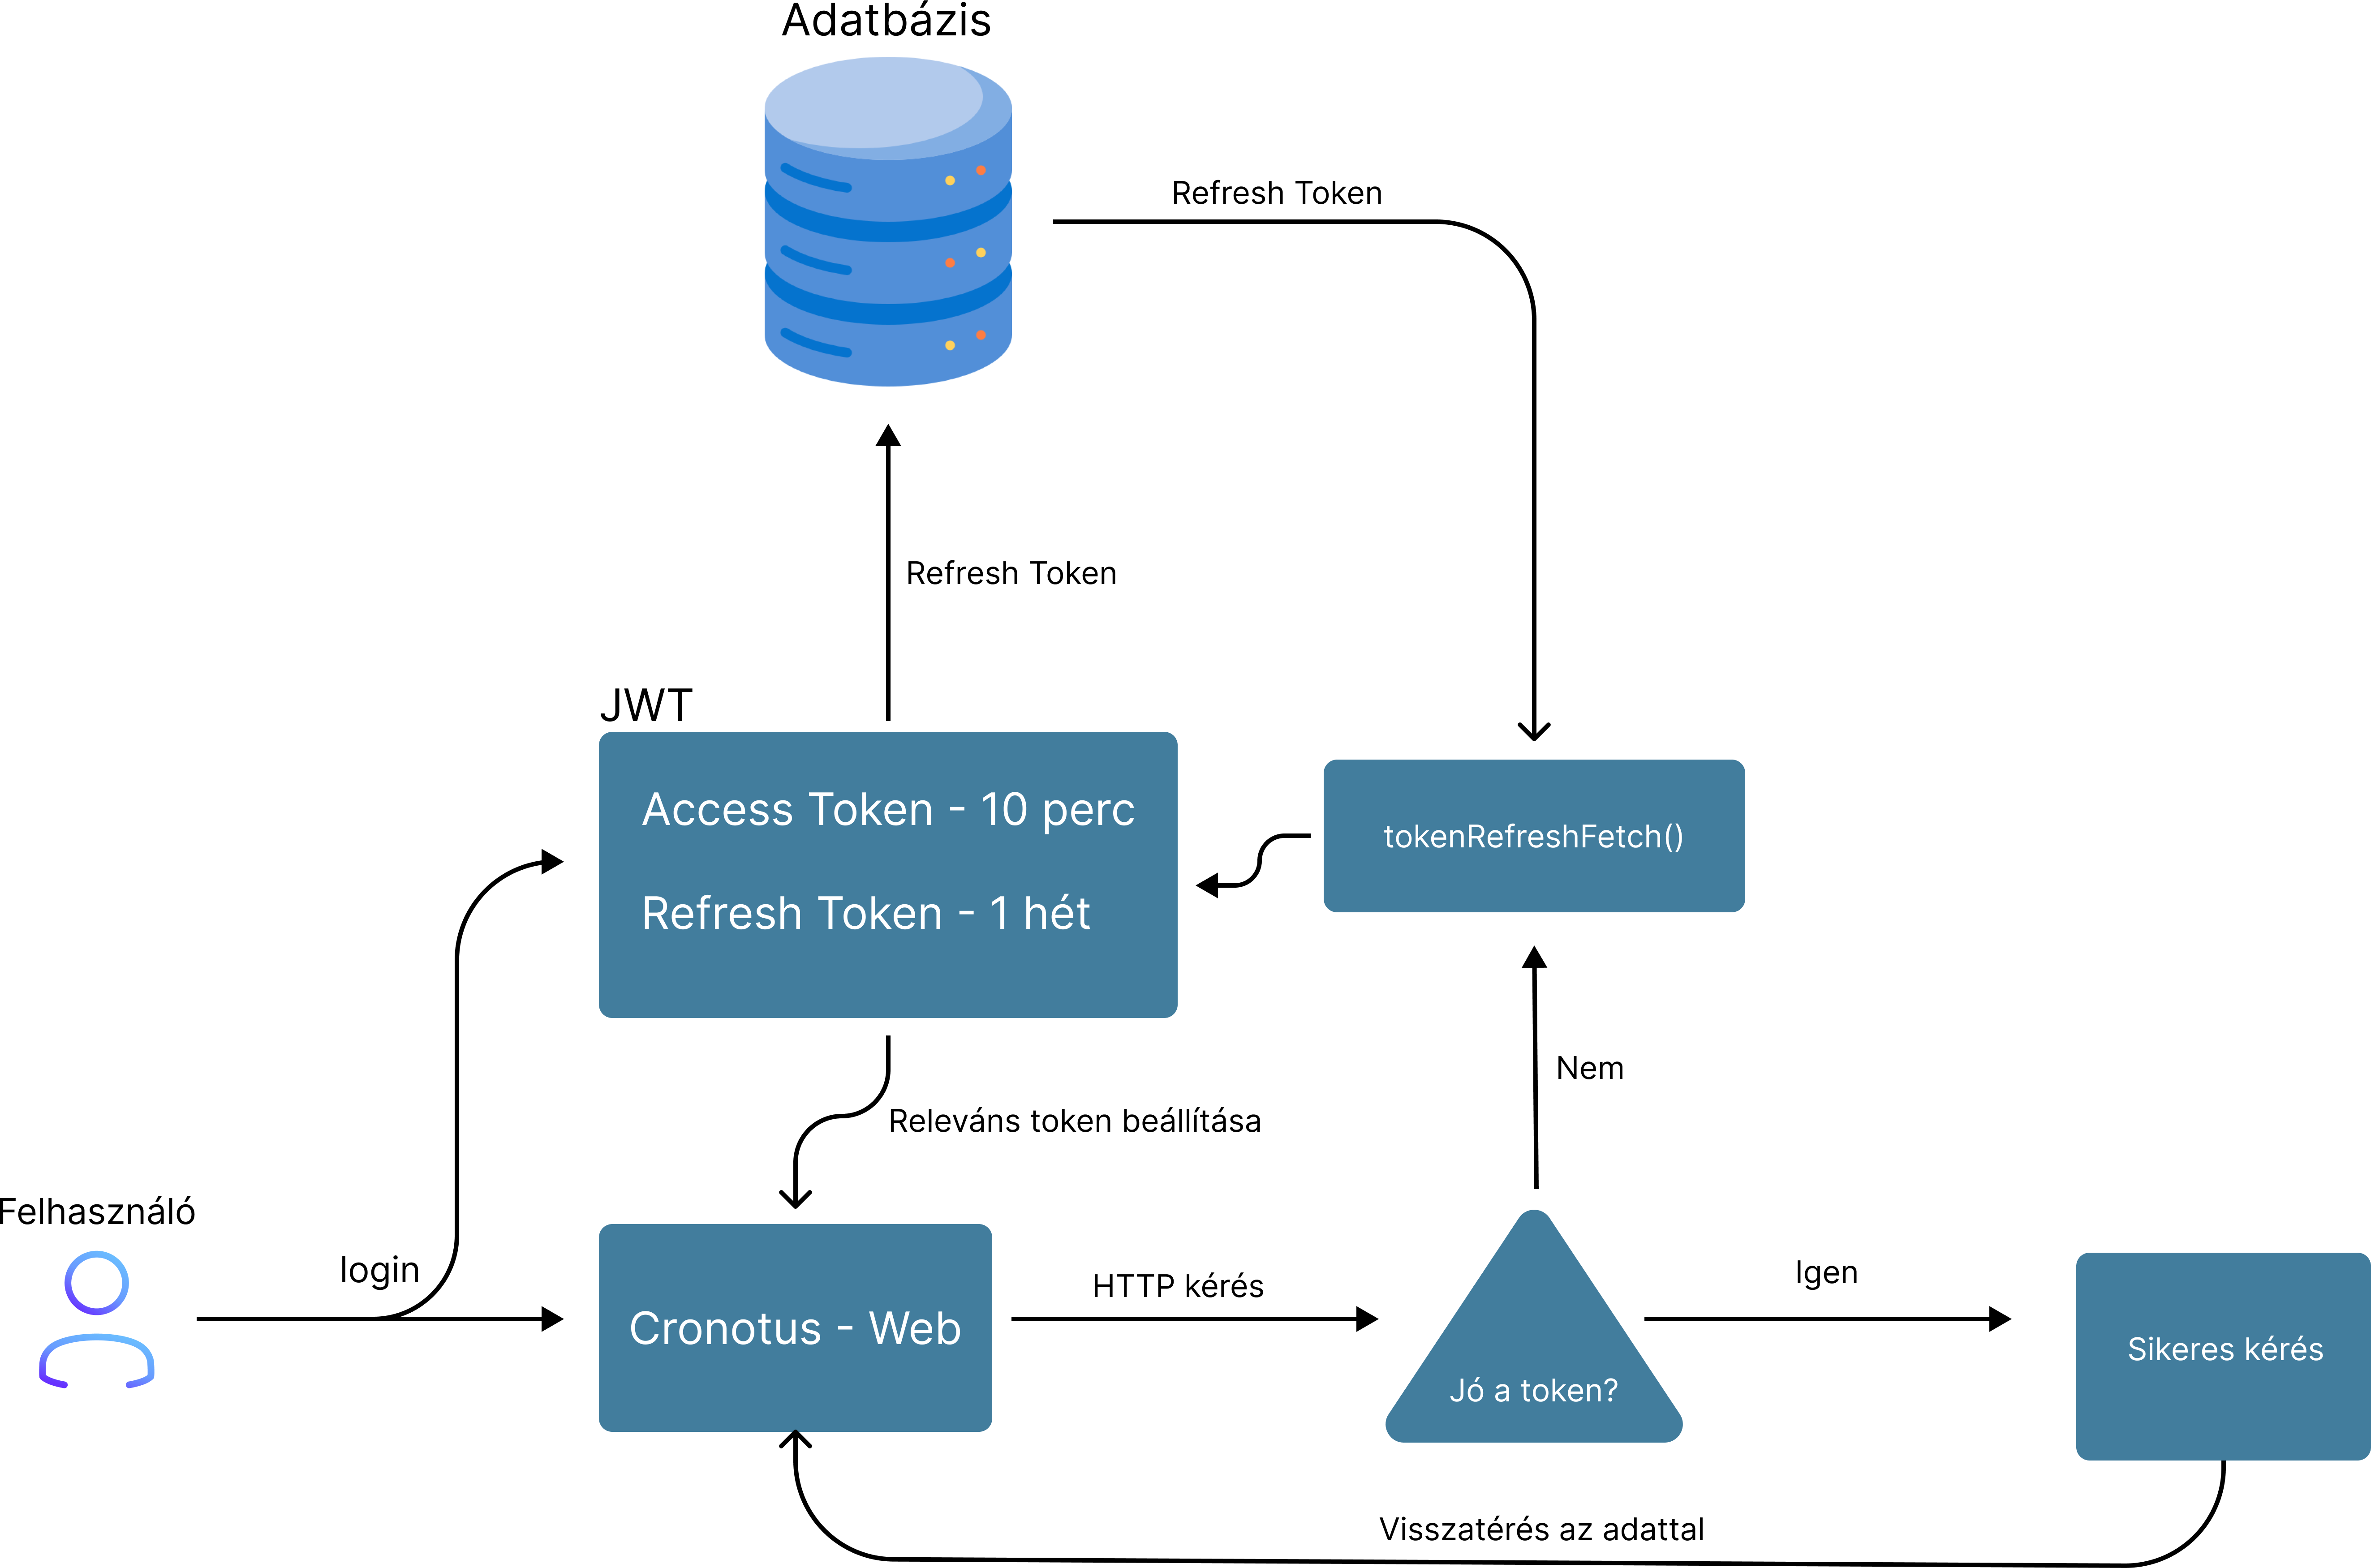
\includegraphics[width=\textwidth]{images/jwt_auth_process.png}
  \caption{A JWT munkamenetkezelés folyamata}
  \label{fig:jwt_auth_process}
\end{figure}
%----------------------------------------------------------------------------

  
  \onehalfspacing
\chapter{A Cronotus felhasználói felülete}

\section{A fogadó oldal és a regisztráció}

A webalkalmazásra való látogatás során a felhasználókat egy egyszerű felület fogadja, ahol lehetőségük van új felhasználó regisztrálására,
vagy belépésre egy már meglévő felhasználóval. Ez látható a \ref{fig:landing_page}-es ábrán.

\begin{figure}[h]
	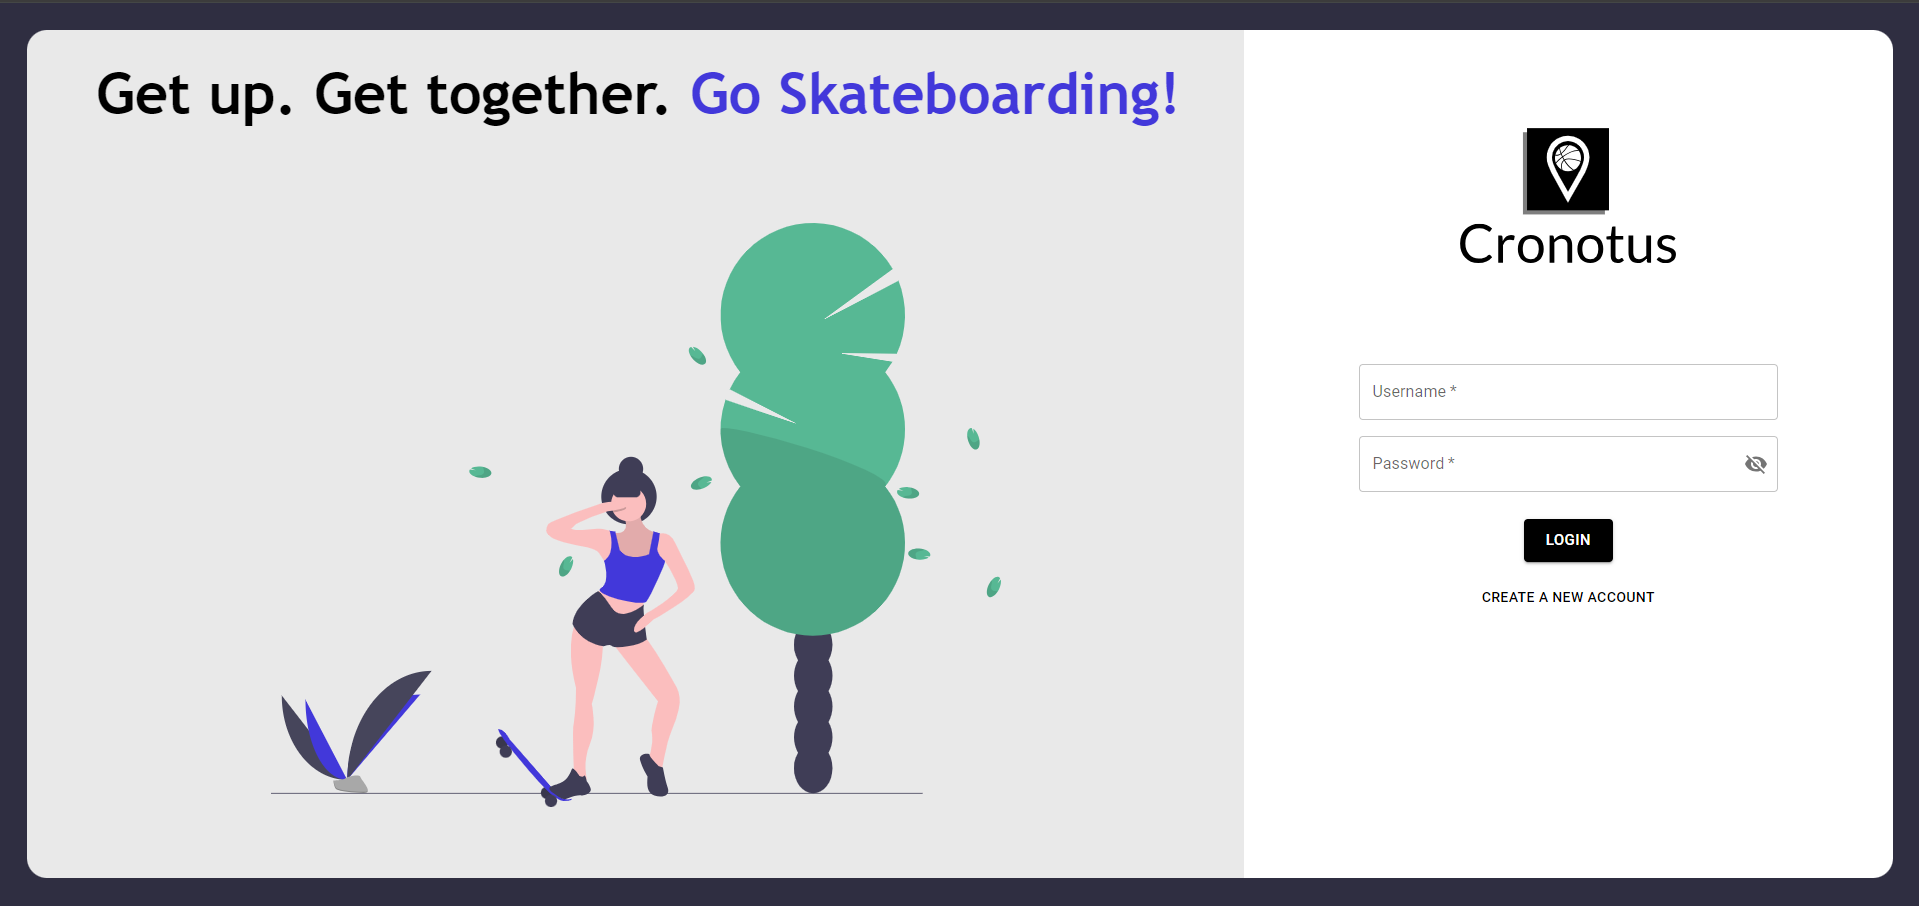
\includegraphics[width=0.5\textwidth]{images/login_page.png}
	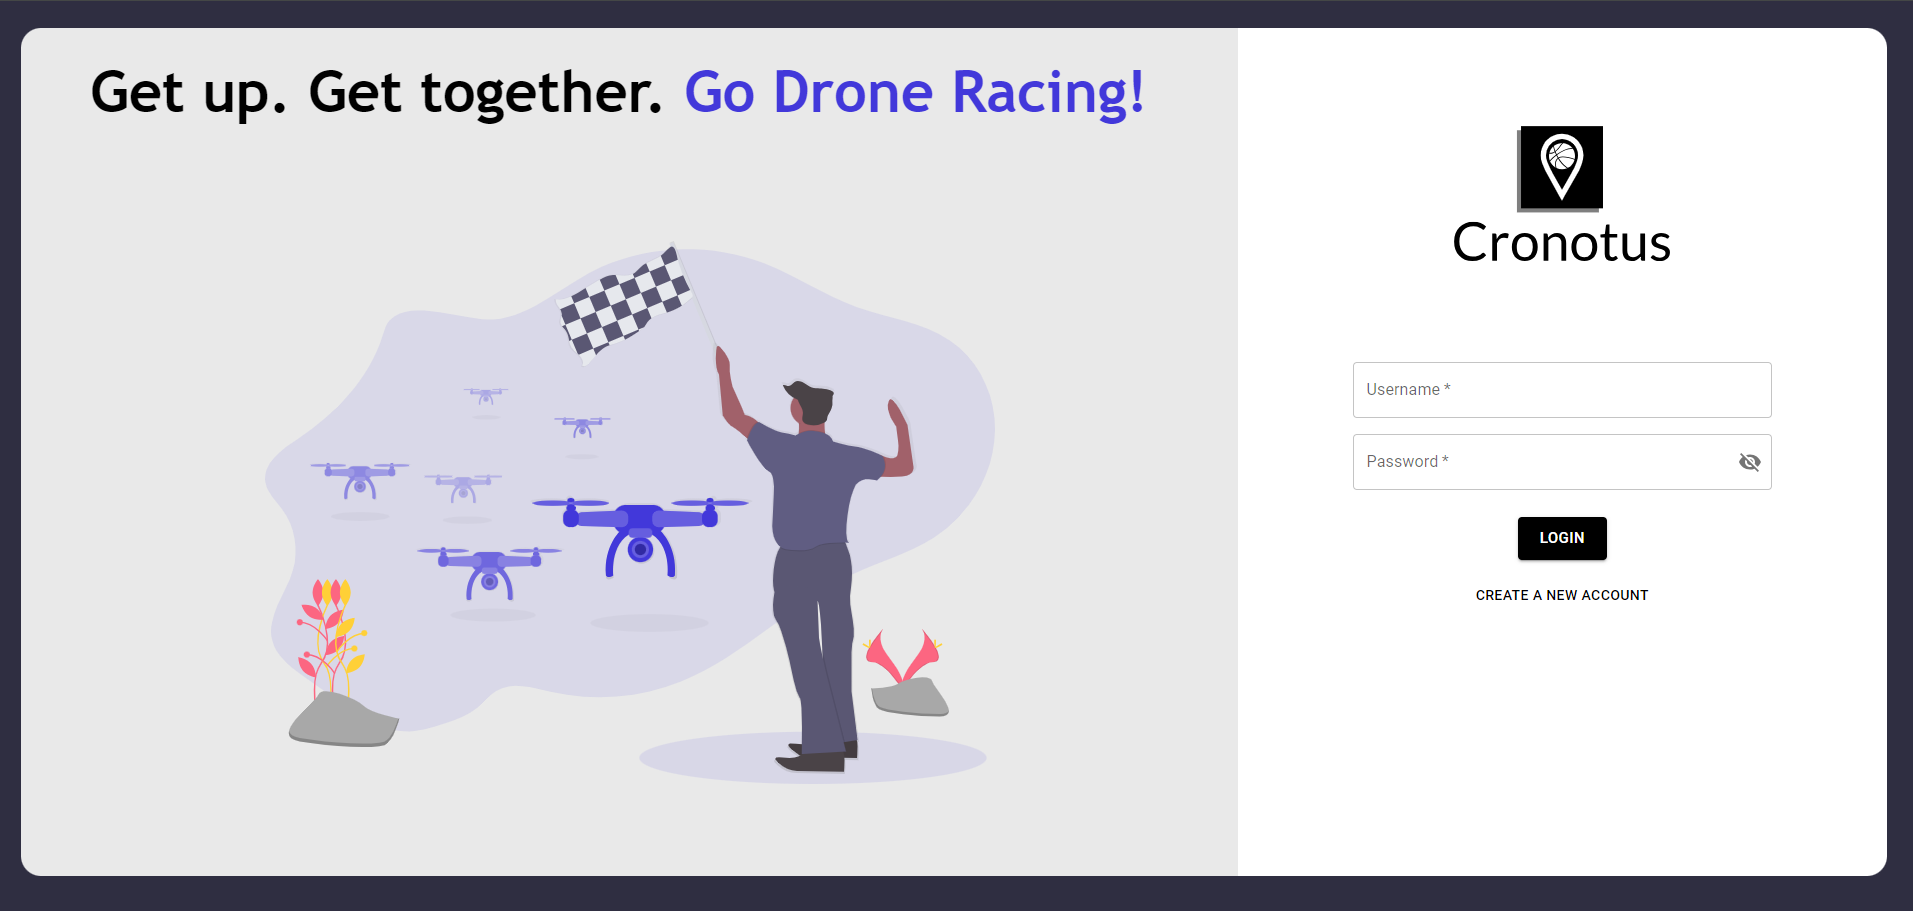
\includegraphics[width=0.5\textwidth]{images/login_2.png}
	\begin{center}
		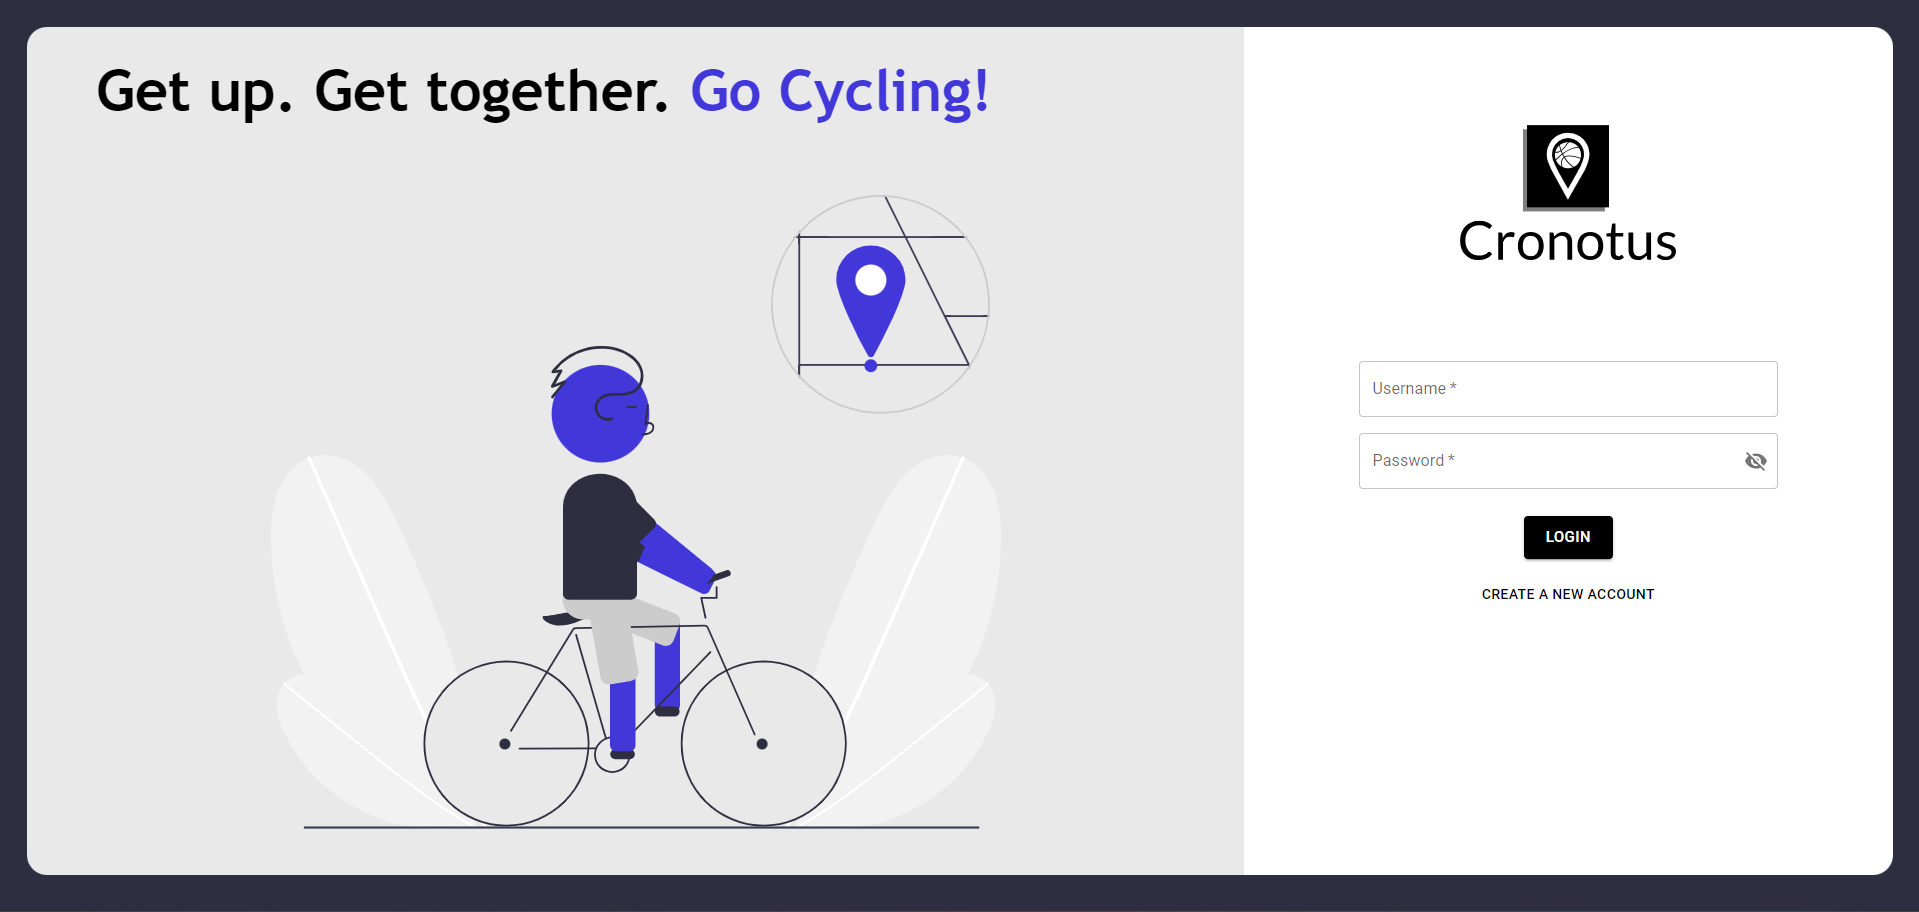
\includegraphics[width=0.7\textwidth]{images/login_3.png}
	\end{center}
	\caption{A fogadó oldal}
	\label{fig:landing_page}
\end{figure}

\newpage


A webalkalmazás igyekszik egy játékos és barátságos hangnemben megnyilvánulni a felhasználók számára. Ez megfigyelhető a regisztrációs folyamaton
is, ami nem egy megszokott űrlap kitöltéséből áll, hanem egyszerű nyelvezettel megfogalmazott kérdések sorozatával segíti a felhasználókat
a regisztráció során. \ref{fig:registration_seq}-es ábra

\begin{figure}[h]
	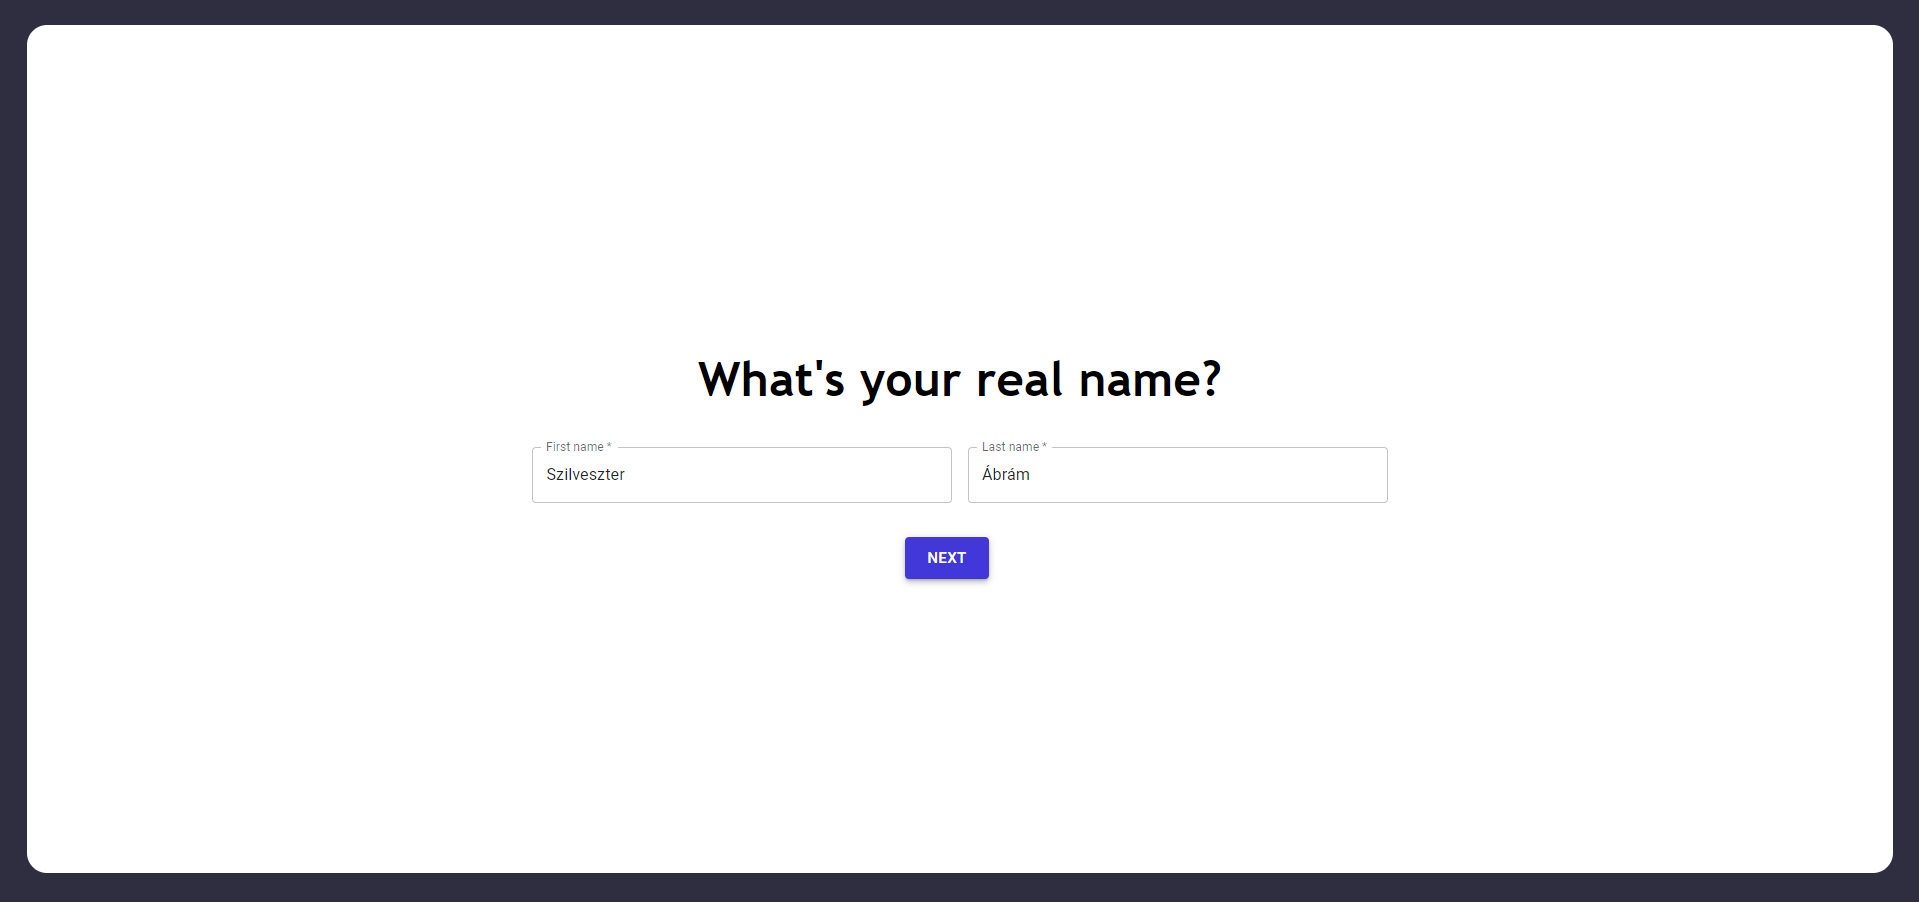
\includegraphics[width=0.5\textwidth]{images/register_1.png}
	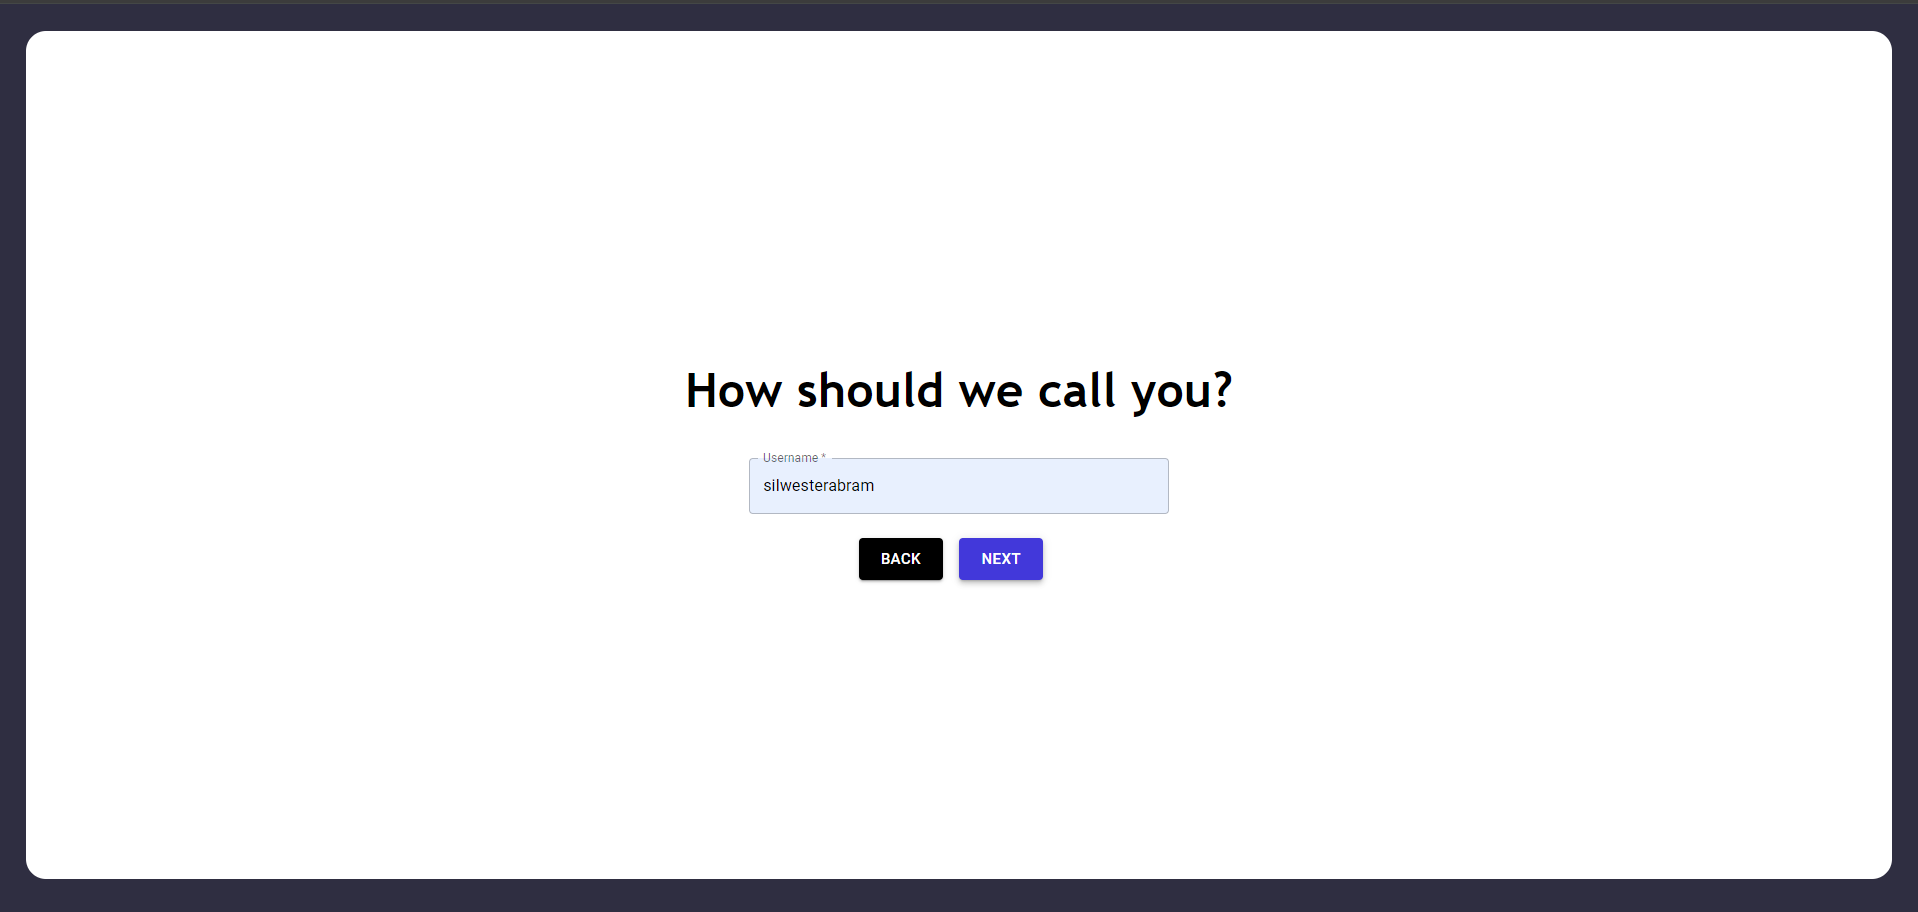
\includegraphics[width=0.5\textwidth]{images/register_2.png}
	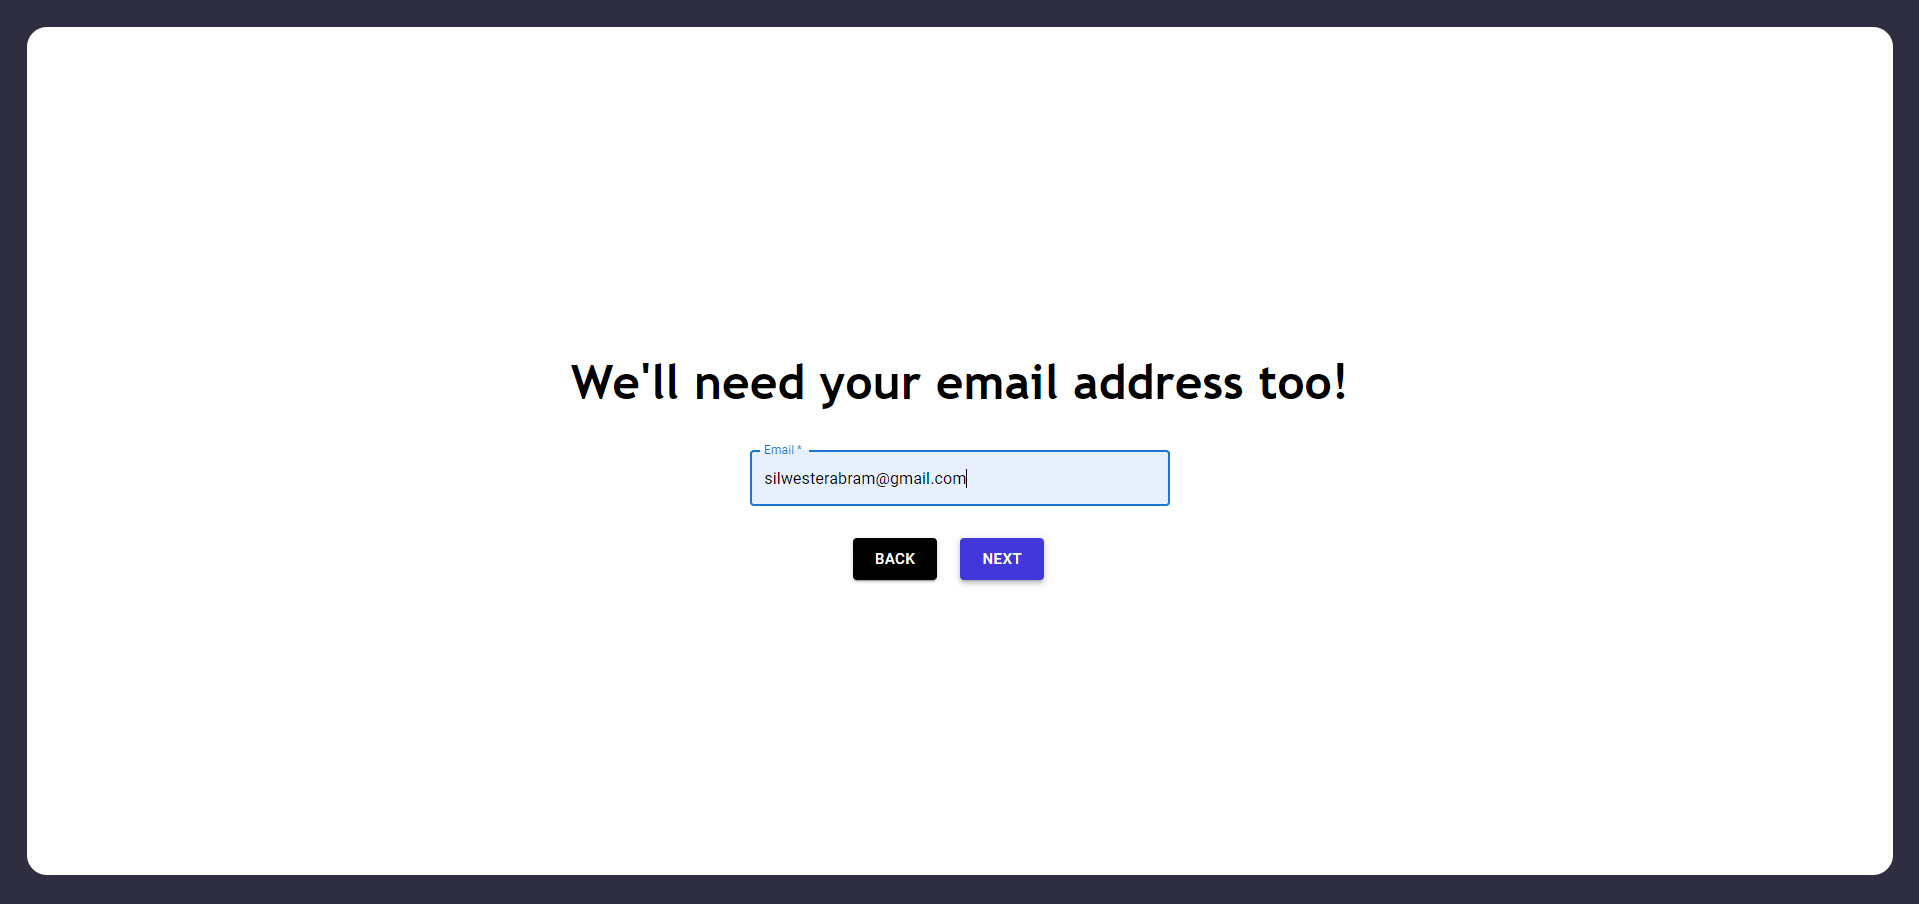
\includegraphics[width=0.5\textwidth]{images/register_3.png}
	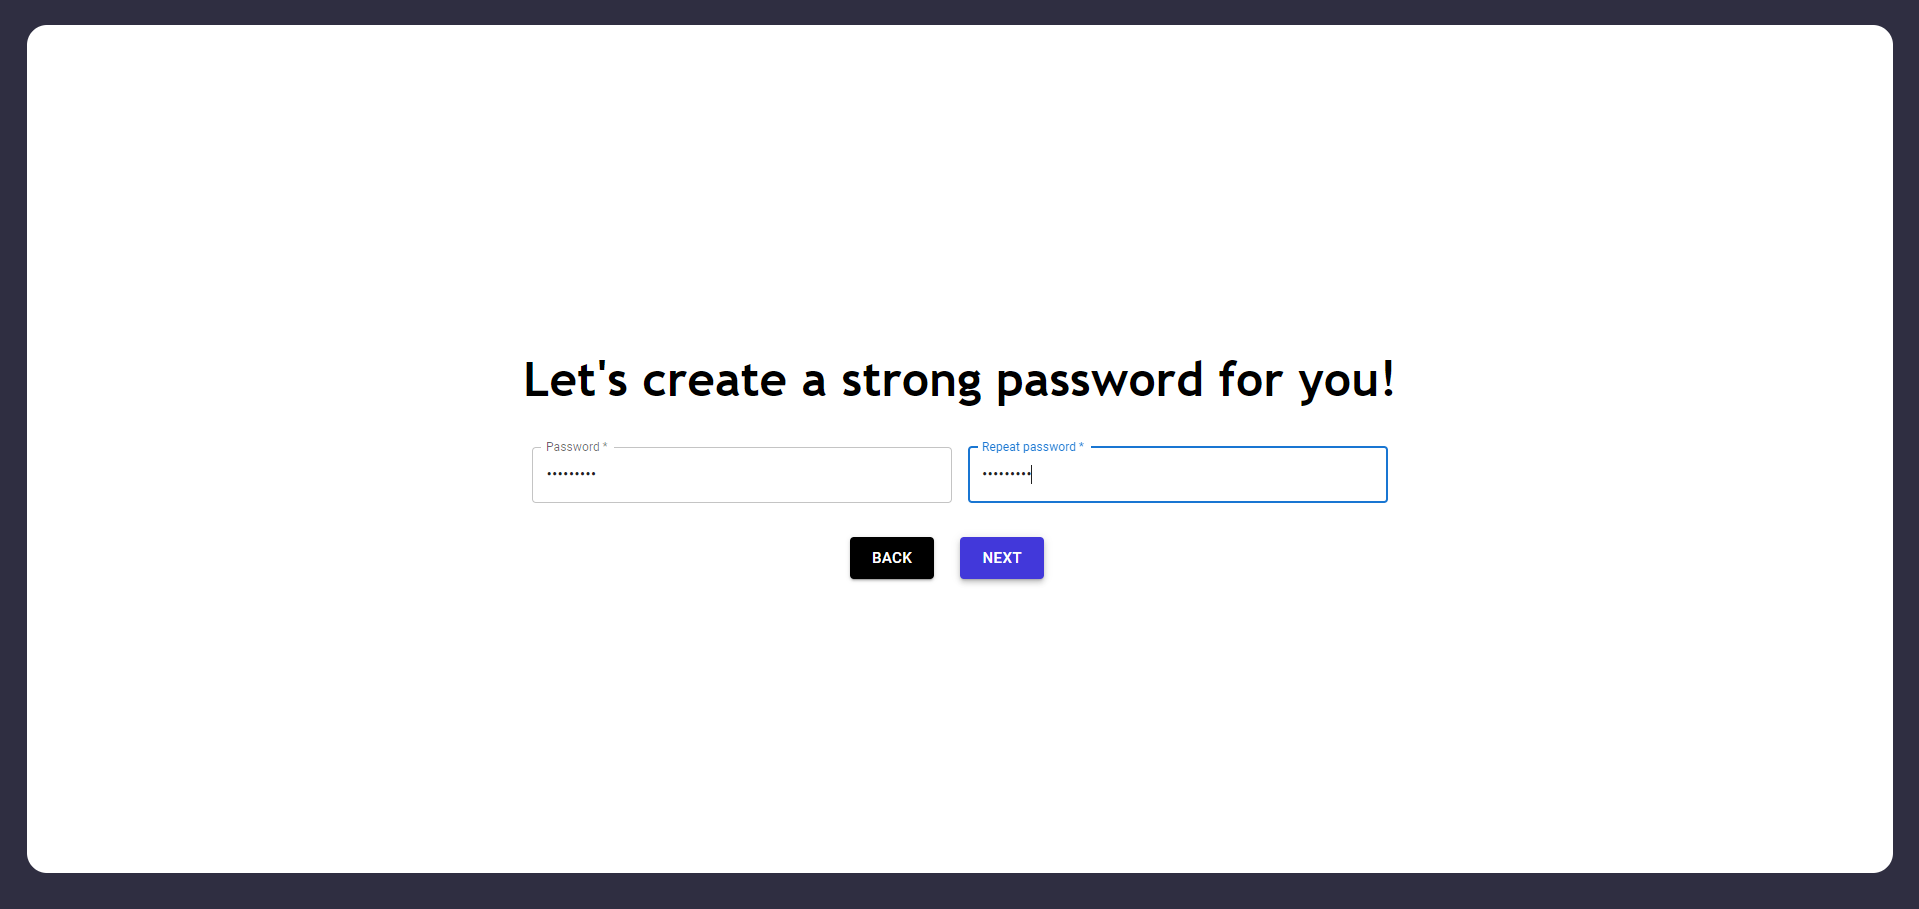
\includegraphics[width=0.5\textwidth]{images/register_4.png}
	\begin{center}
		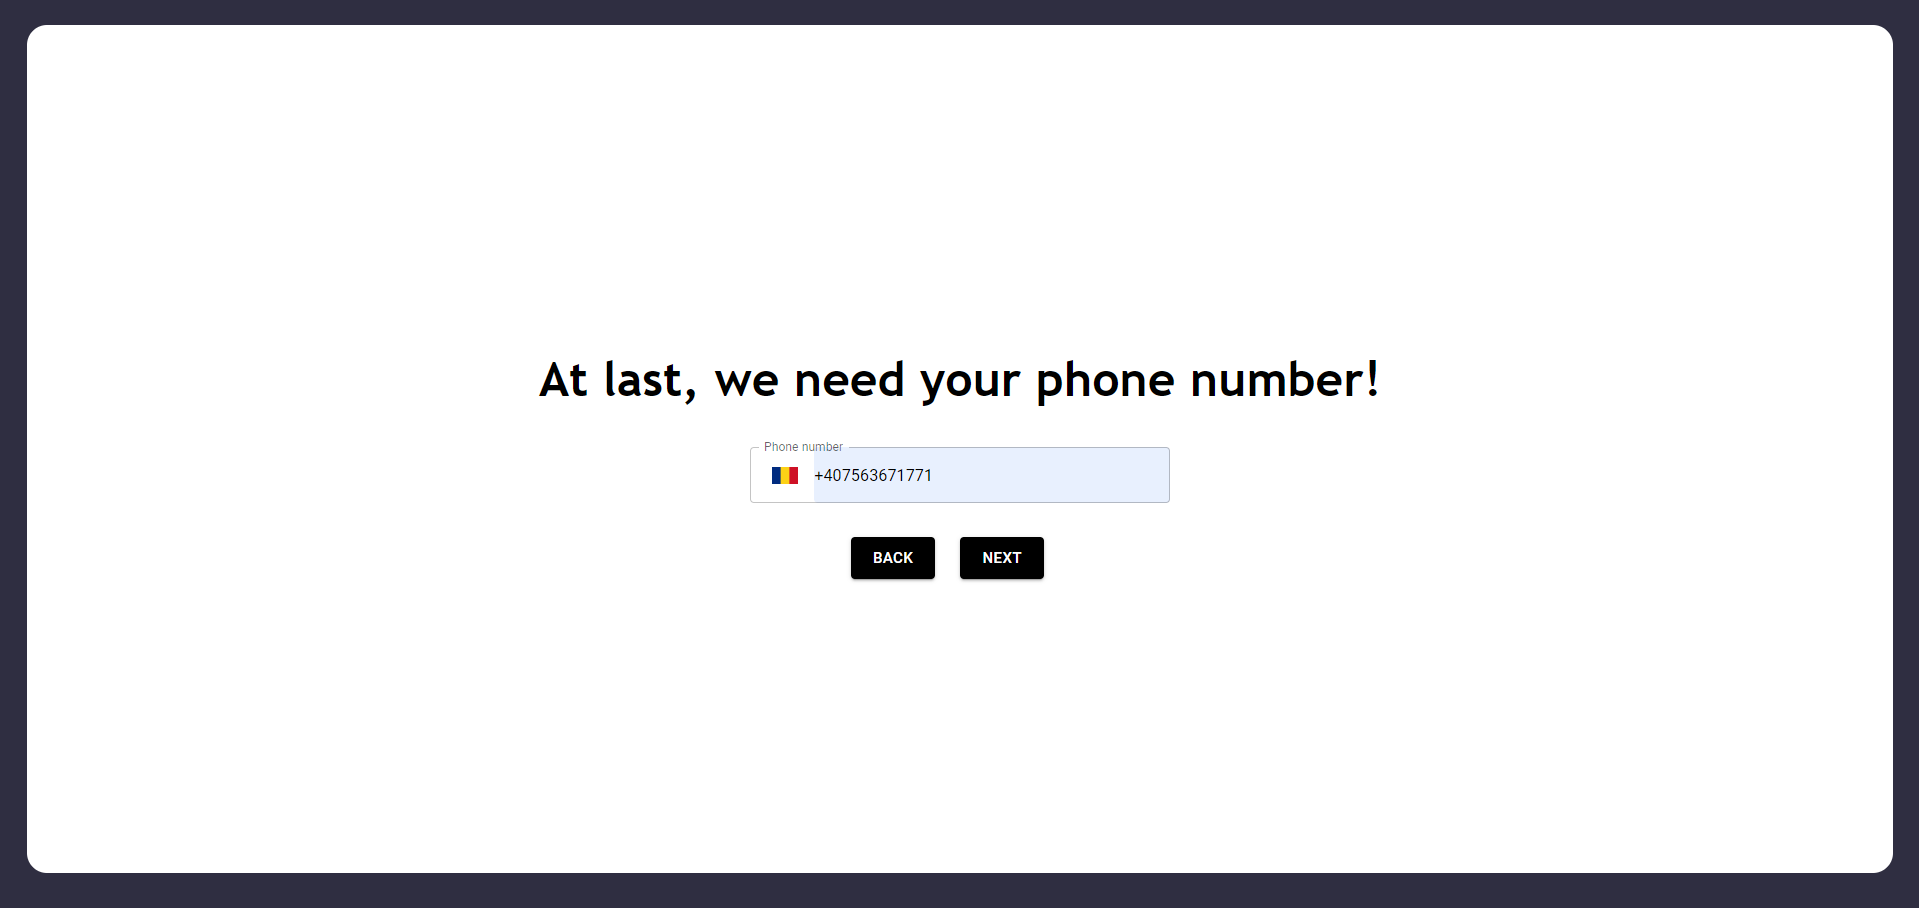
\includegraphics[width=0.5\textwidth]{images/register_5.png}
	\end{center}
	\caption{A regisztrációs folyamat}
	\label{fig:registration_seq}
\end{figure}

\newpage

\section{A profil oldal}

A regisztráció alkalmával megadott információk megtekinthetők a profil oldalon. Itt lehetőség van arra is, hogy a felhasználó megváltoztassa a személyes
információit, illetve profil és borítóképét is. Ez látható a \ref{fig:profile_page}-as ábrán.

\begin{figure}[ht]
	\centering
	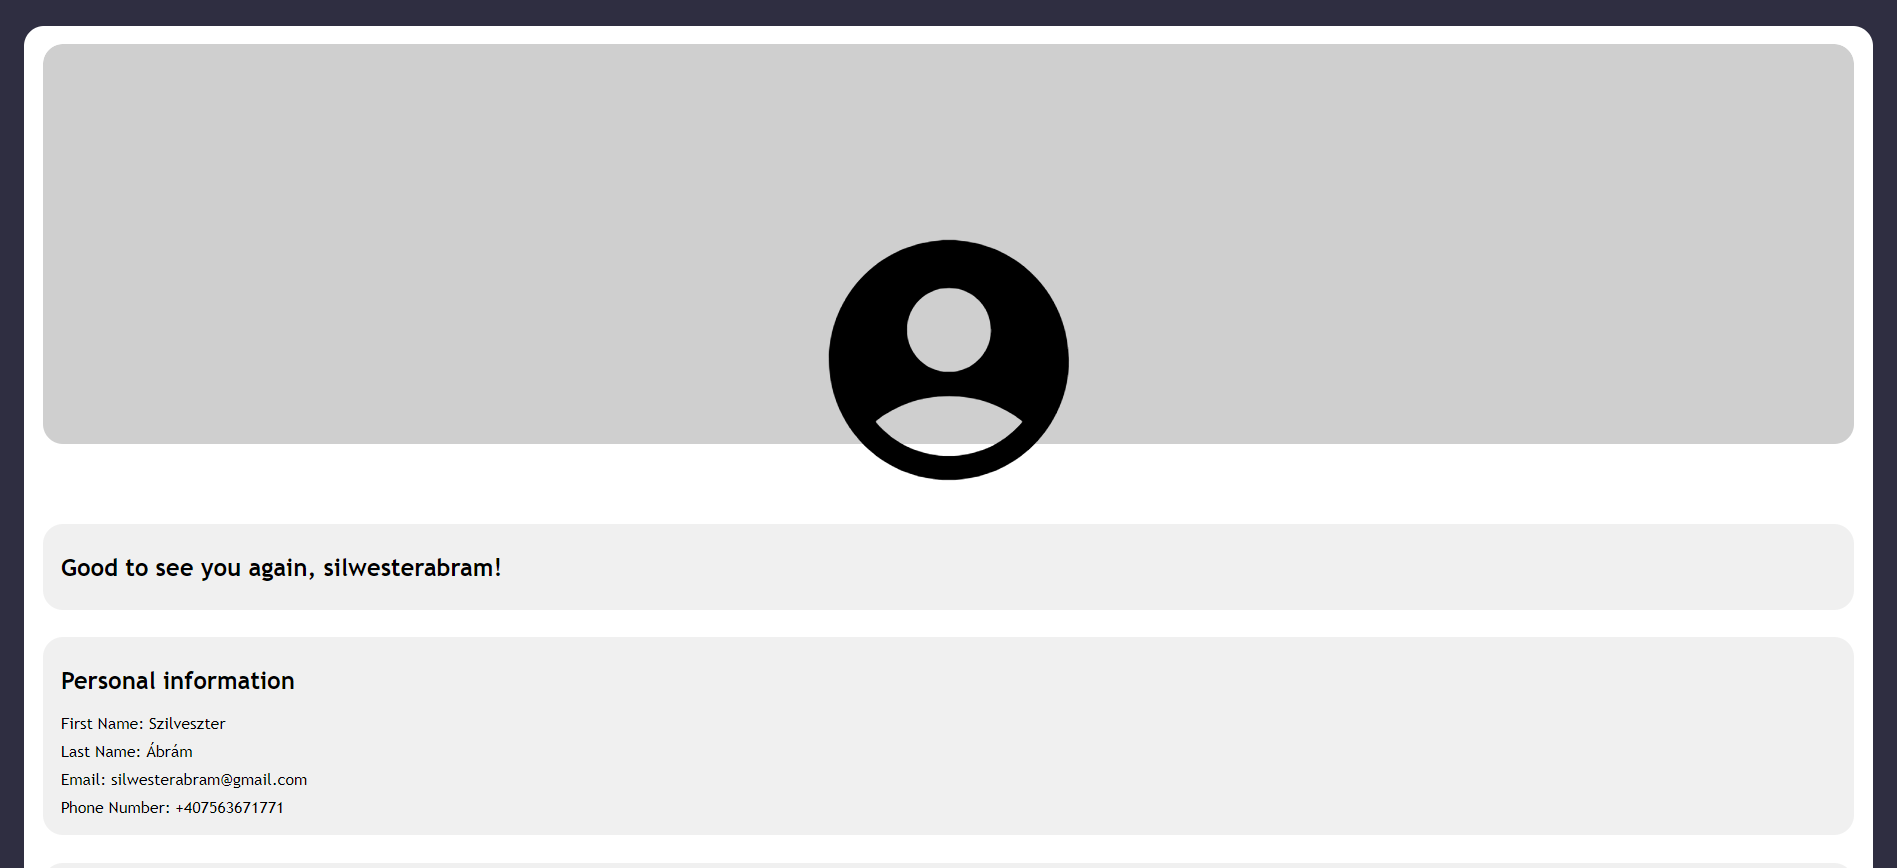
\includegraphics[width=0.6\textwidth]{images/profile_1.png}
	\caption{A profil oldal}
	\label{fig:profile_page}
\end{figure}

A Profil oldalon való ``Edit Profile''-ra való kattintással előhozható egy felület, ahol a felhasználó megváltoztathatja személyes információit,
illetve lehetősége van arra is, hogy profil és borítóképet változtasson, hogy egyéni stílusát tükrözze a felületen. Ez látható a 
\ref{fig:profile_edit_page}-es ábrán.

\begin{figure}[h]
		\centering
		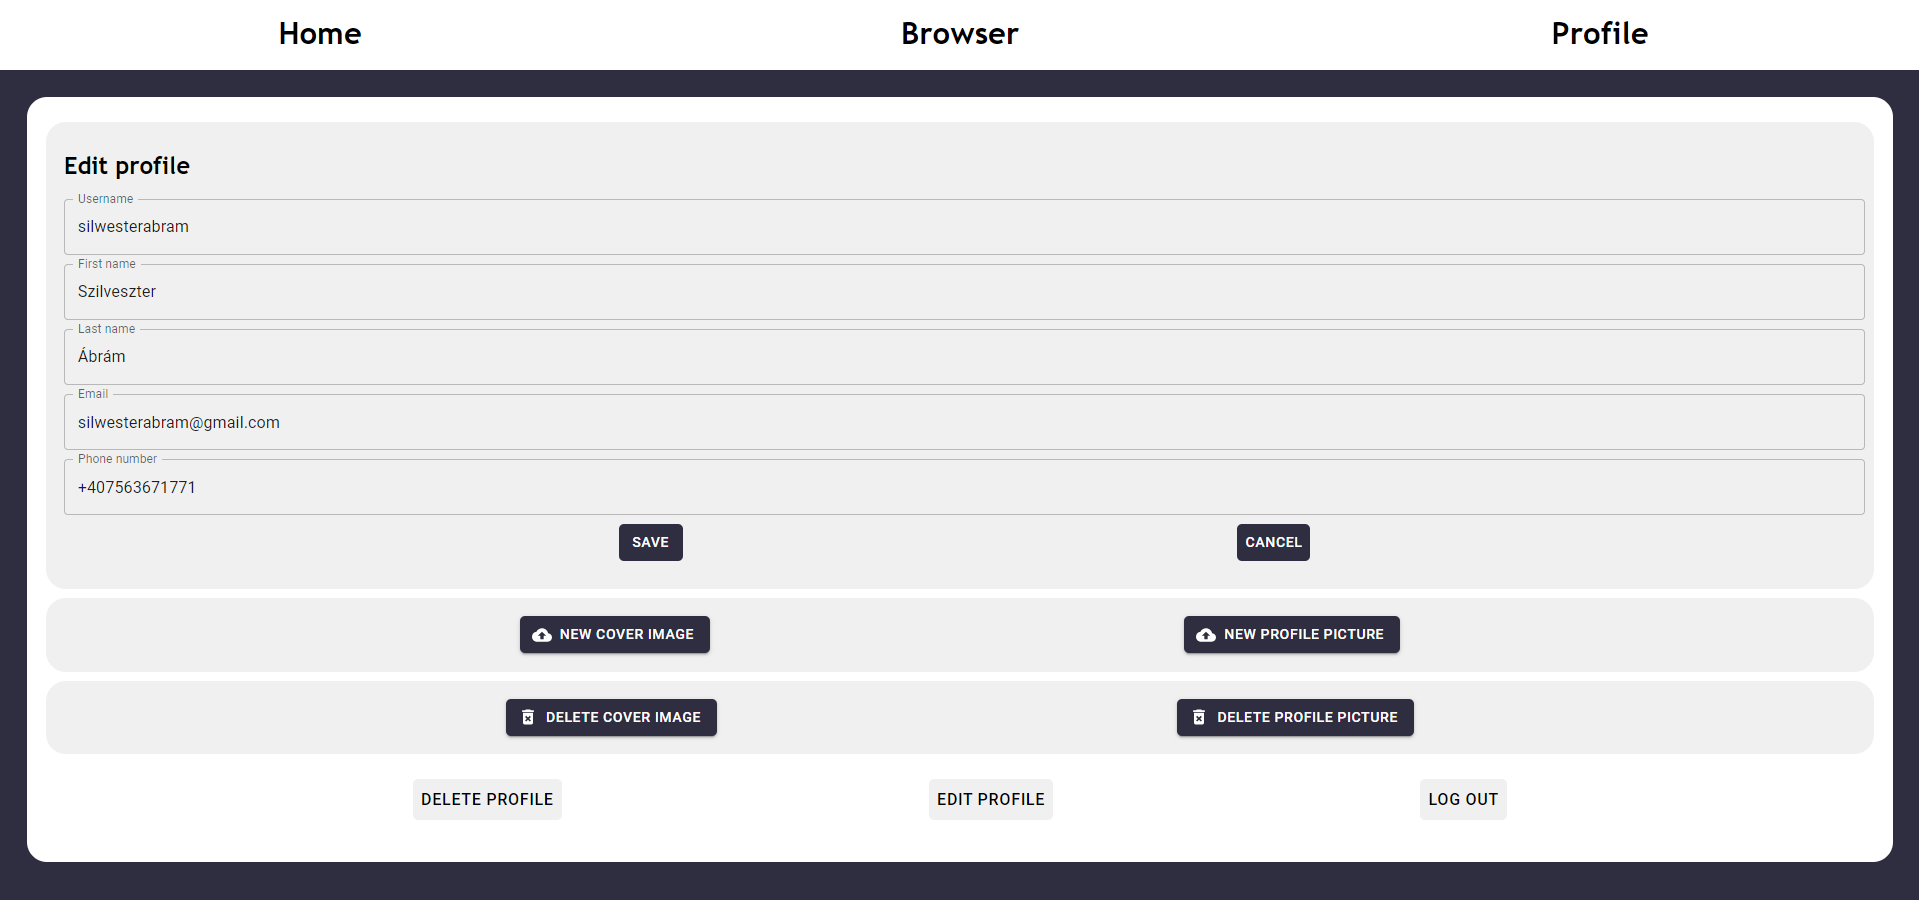
\includegraphics[width=0.6\textwidth]{images/profile_edit.png}
		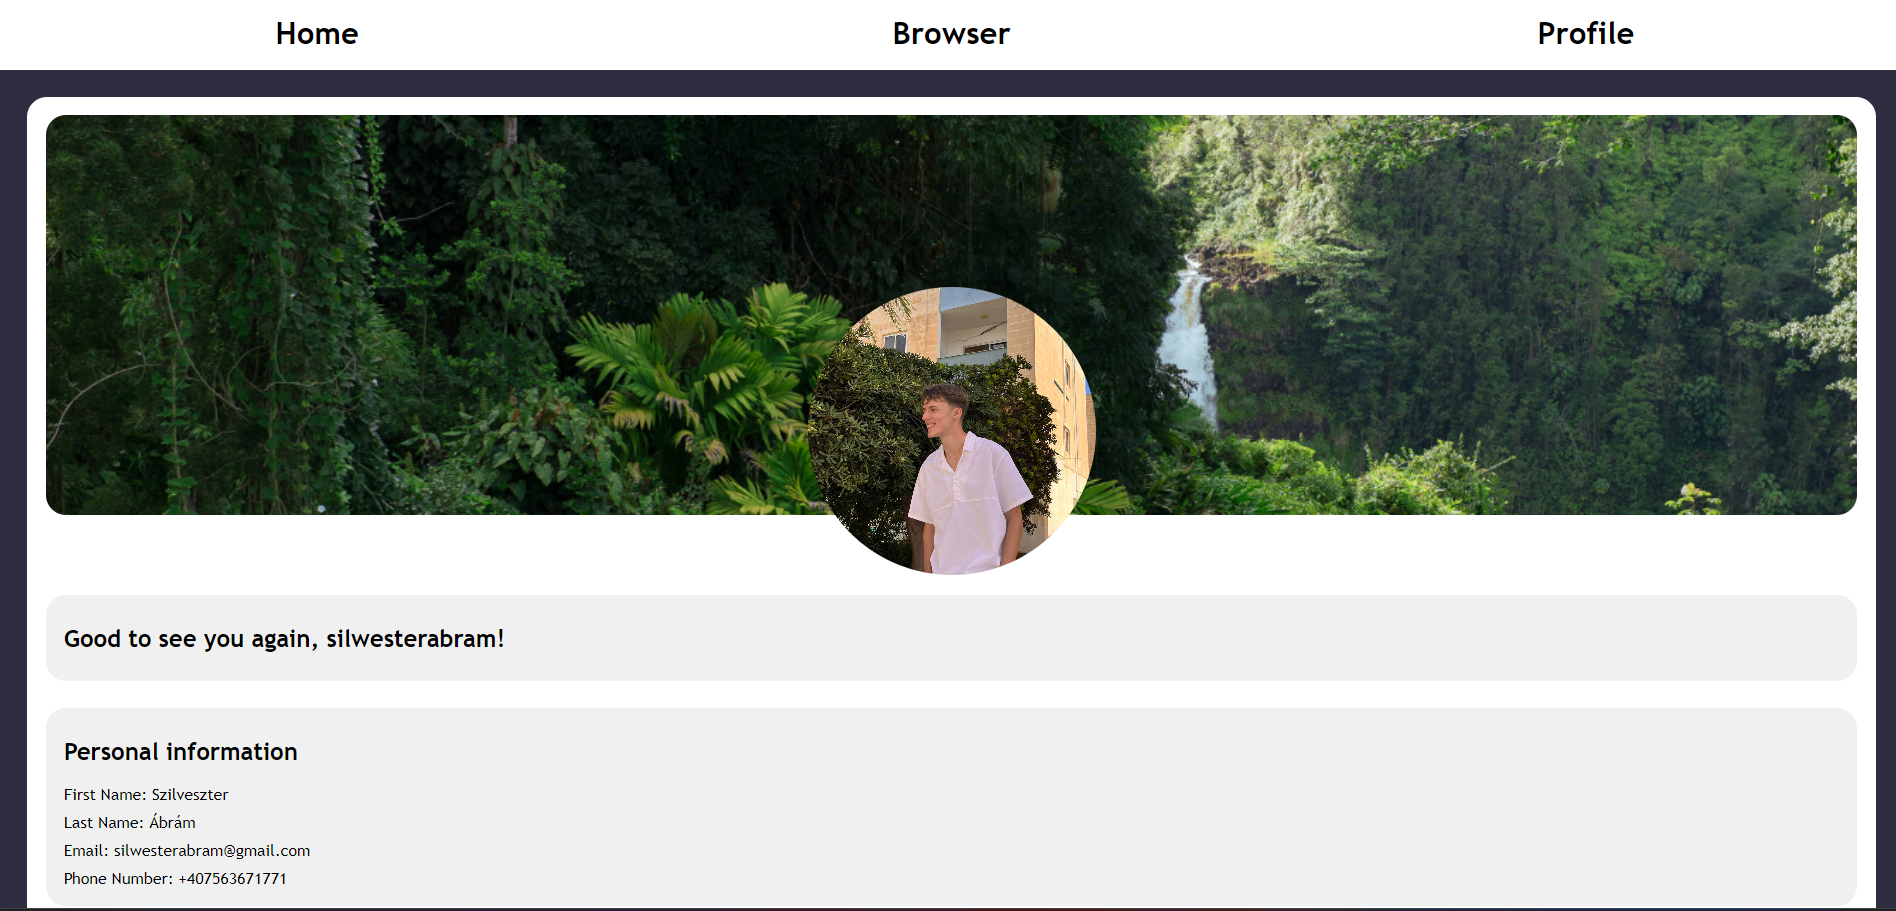
\includegraphics[width=0.6\textwidth]{images/profile_2.png}
	\caption{A profil szerkesztése}
	\label{fig:profile_edit_page}
\end{figure}

A továbbiakban lehetőségünk van a felhasználónk törlésére is. A ``Delete Profile'' gomb megnyomásával előhozható egy prompt, 
amit ha továbbra is megerősítünk, akkor egyszerűen törölhetjük a felhasználónkat, s minden vele kapcsolatos információt, eseményt. [\ref{fig:delete_profile}-ös ábra]

\begin{figure}
	\centering
	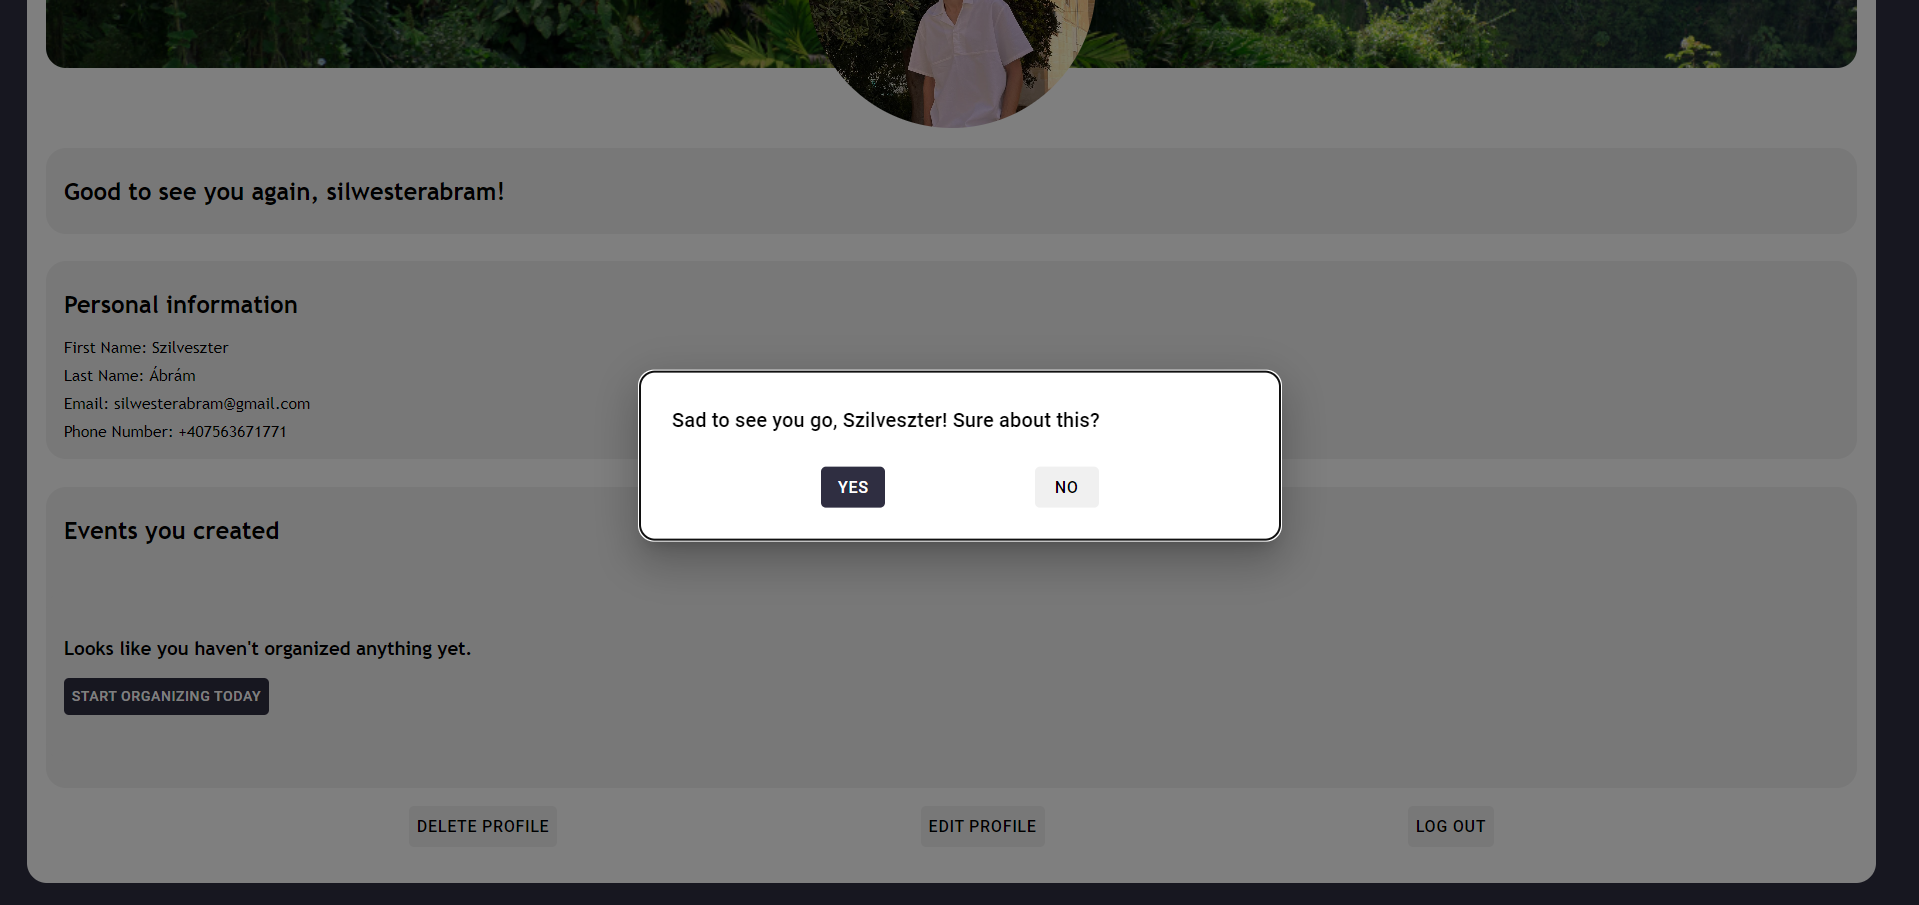
\includegraphics[width=0.7\textwidth]{images/delete_profile.png}
	\caption{A profil törlése}
	\label{fig:delete_profile}
\end{figure}

Az oldal listázza az általunk szervezett sporteseményeket is. Mivel egy újonnan létrehozott felhasználónk van, még nem hoztunk létre egyetlen
sporteseményt sem, így a lista üres. Ilyenkor ezt jelzi nekünk az oldal, illetve ennek megfelelően jelenít meg egy gombot, amivel átirányít
bennünket arra a felületre, ahol létrehozhatunk új sporteseményeket. [\ref{fig:profile_page_2}-os ábra]

\begin{figure}[h]
	\centering
	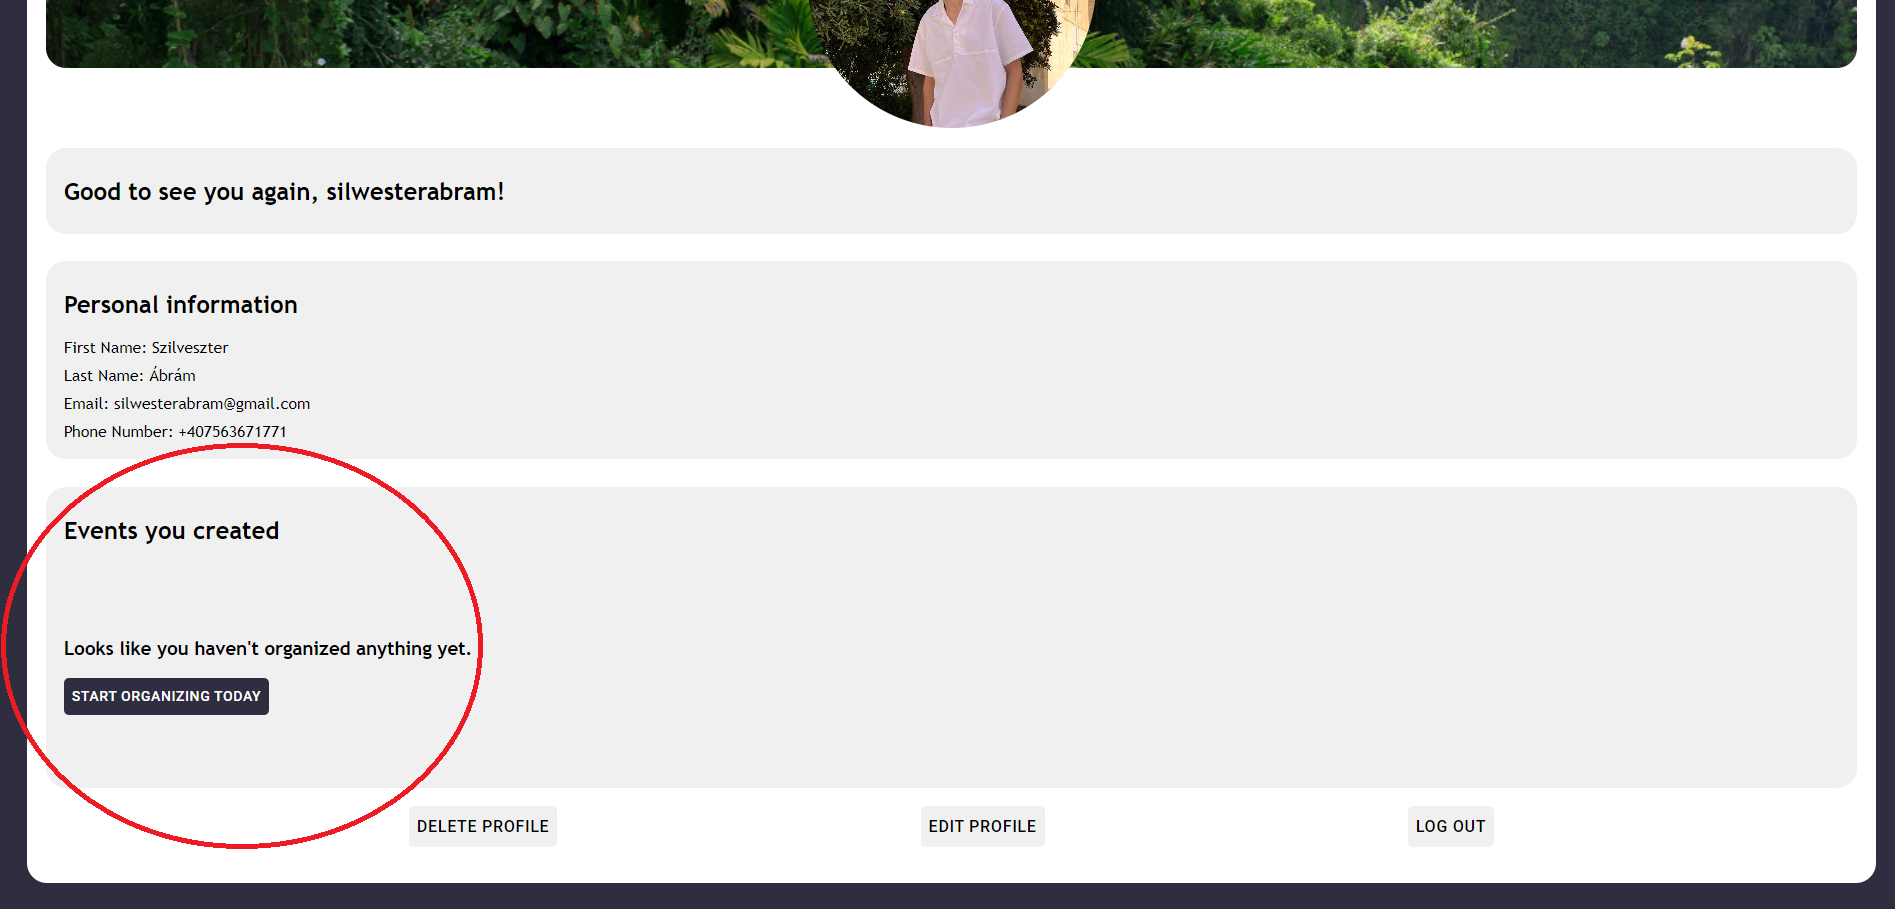
\includegraphics[width=0.7\textwidth]{images/events_by_you_profile.png}
	\caption{Általunk szervezett sportesemények listázása a profil oldalon}
	\label{fig:profile_page_2}
\end{figure}

\section{A sportesemény böngésző}

A sportesemény böngésző, azaz a ``Browser'' oldal két fő részre osztható. A ``See what others are up to'' fül alatt listázhatjuk az összes
létrehozott sporteseményt, míg a ``Create a new event'' lehetőséget ad arra, hogy létrehozhassuk egy új, saját eseményt.
Ez látható a \ref{fig:browser_page}-es ábrán is.

\newpage

\begin{figure}[ht]
	\centering
	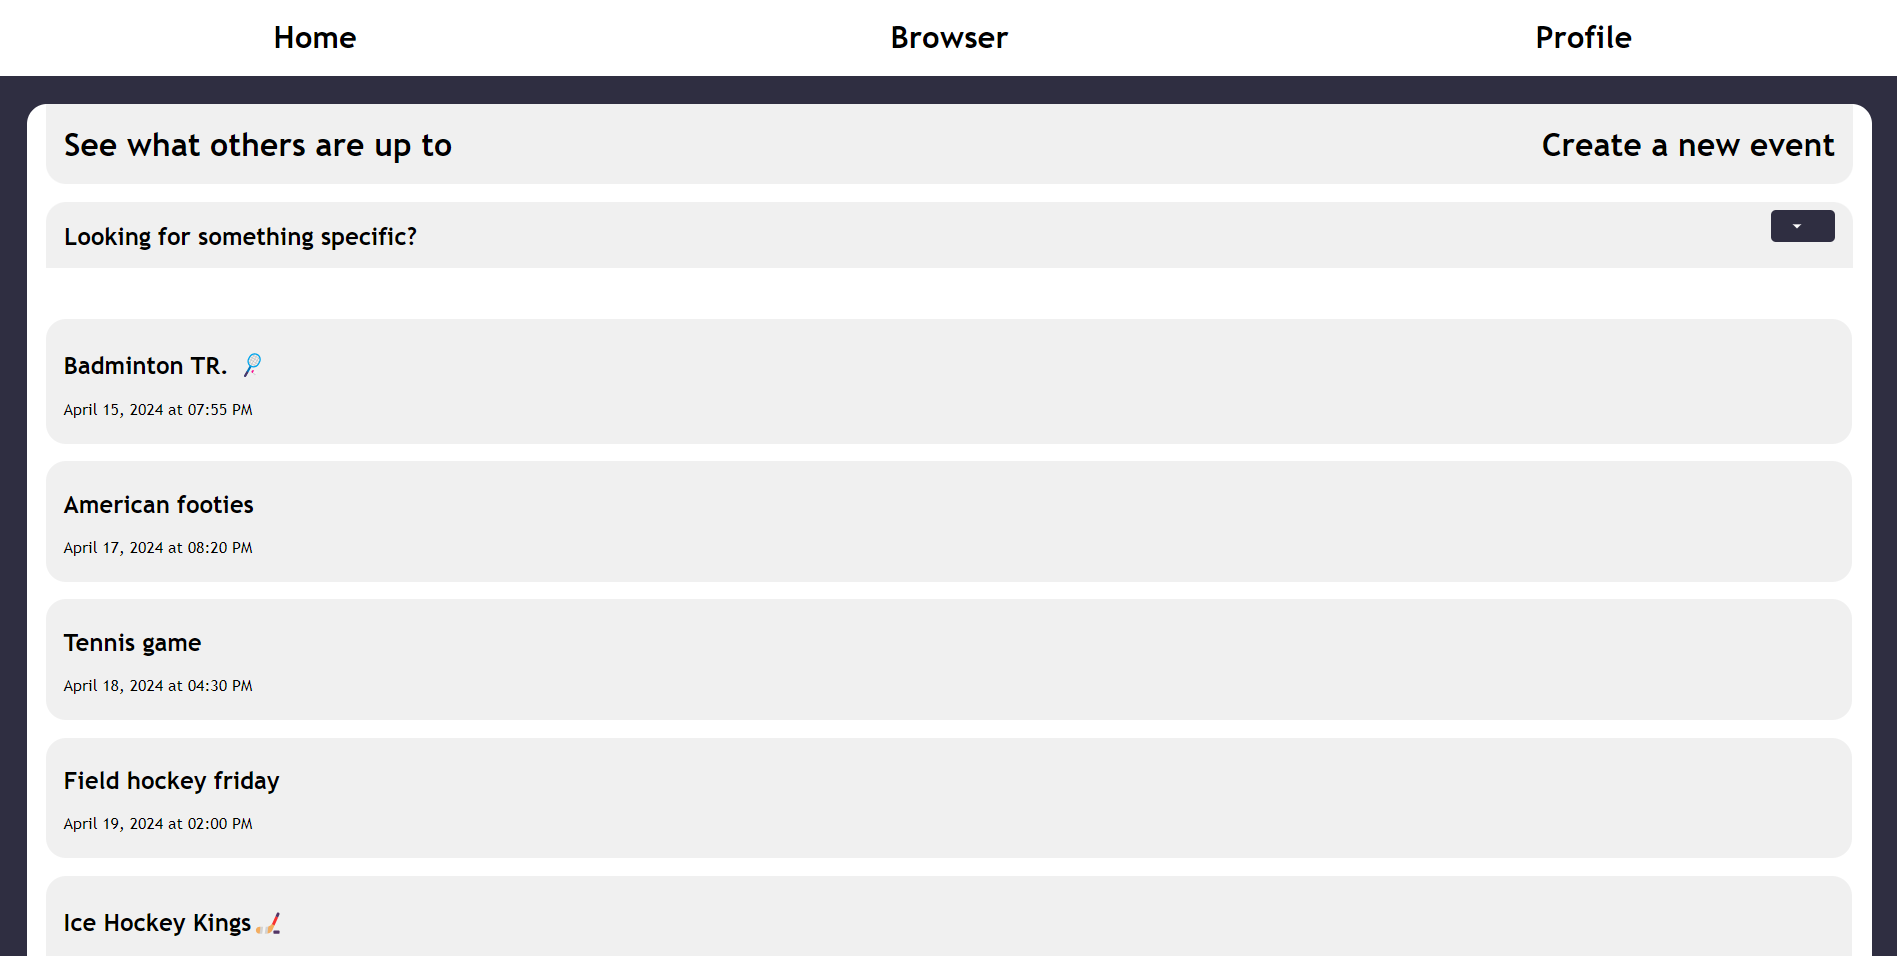
\includegraphics[width=0.7\textwidth]{images/browser_page.png}
	\caption{A sportesemény böngésző}
	\label{fig:browser_page}
\end{figure}

Egy új esemény létrehozása során egy egyszerű űrlapot kell kitöltenie a felasználónak. Itt meglévő sportok közül választhat, az esemény témájaként.
Megfelelő információk, sport, dátum és résztvevőszám megadása után a ``Submit'' gombra kattintás hozhatja létre az általa kívánt eseményt.
Ez a folyamat látható a \ref{fig:create_event}-as ábrán. Az esemény sikeres létrehozása után megfigyelhetjük, hogy az esemény megjelenik a sportesemény böngészőben is. Itt rákattintás segítségével előhozható
egy részletesebb nézet. [\ref{fig:new_event_created}-es ábra]

\begin{figure}[h]
	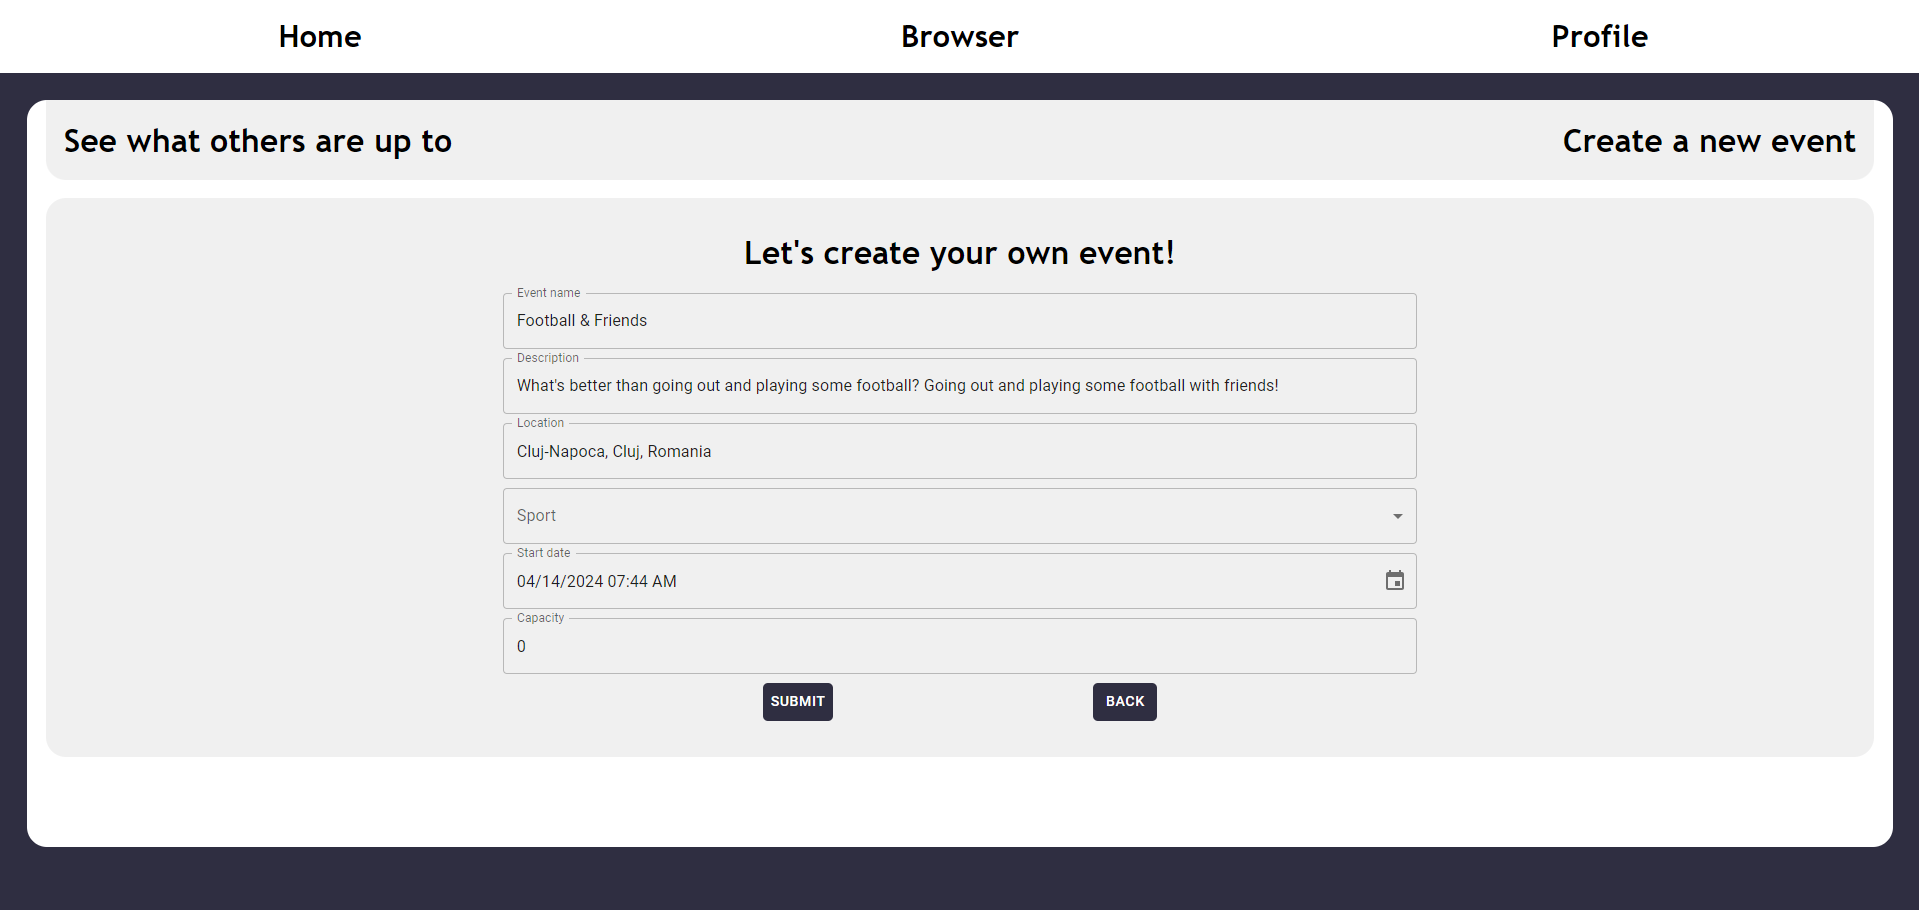
\includegraphics[width=0.5\textwidth]{images/create_event_1.png}
	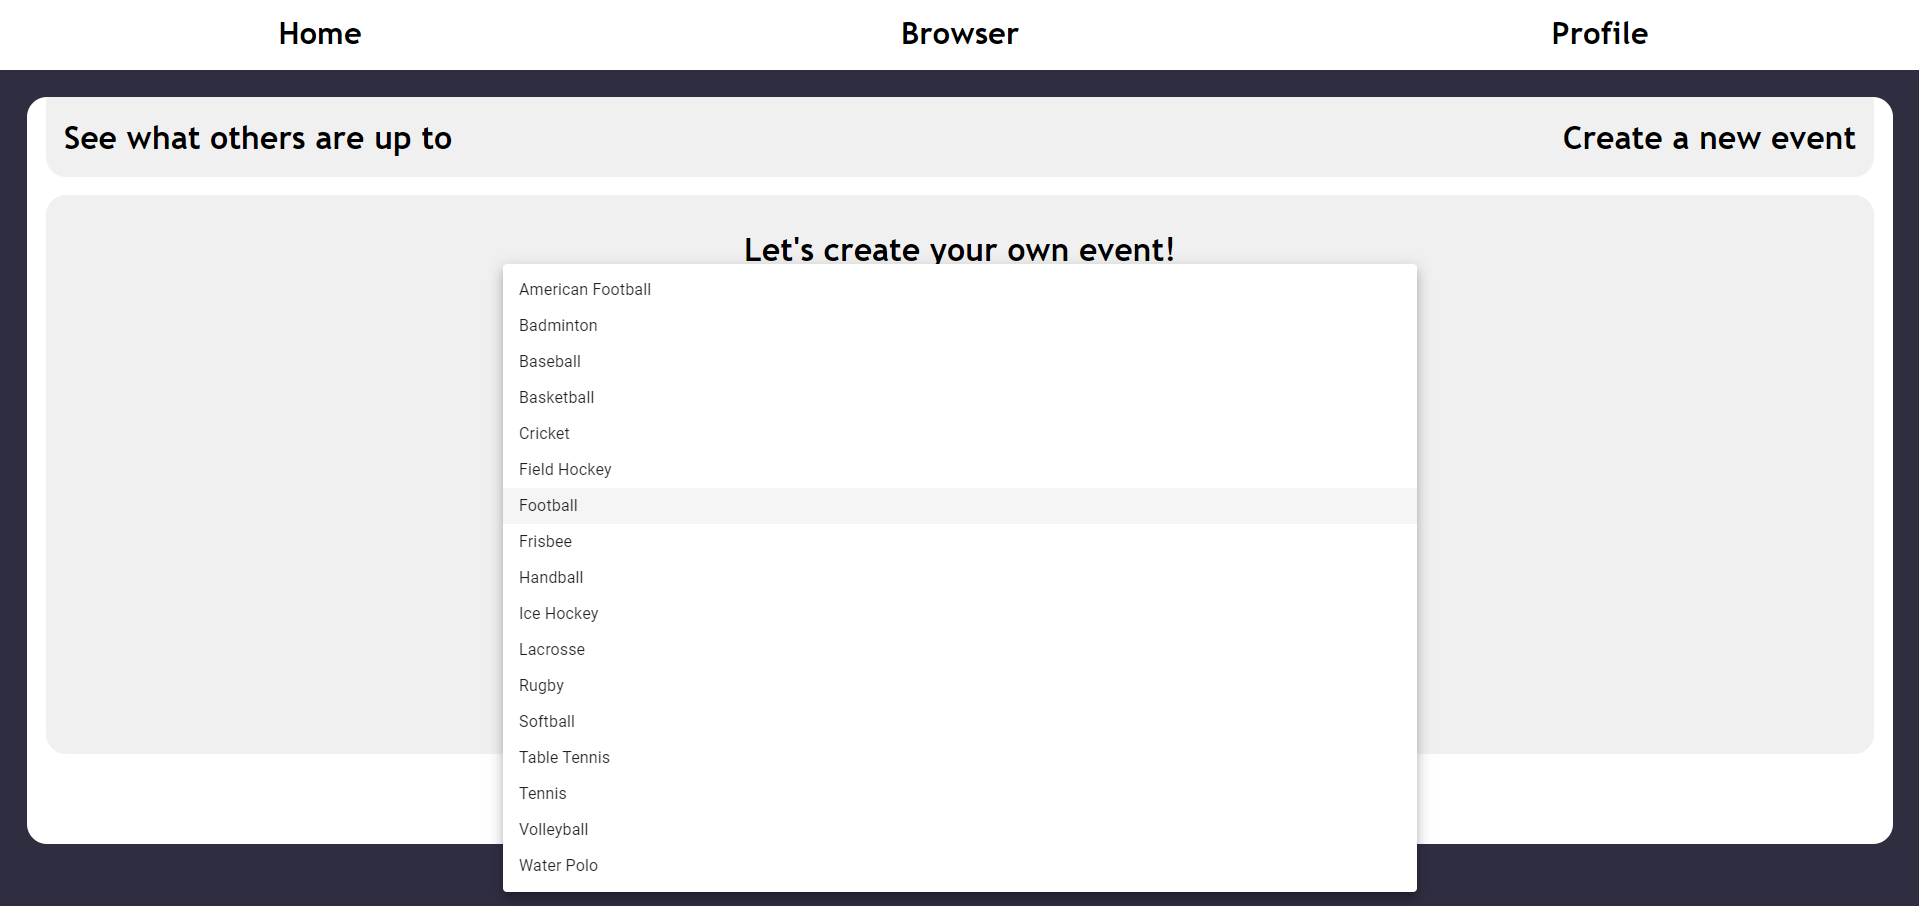
\includegraphics[width=0.5\textwidth]{images/create_event_2.png}
	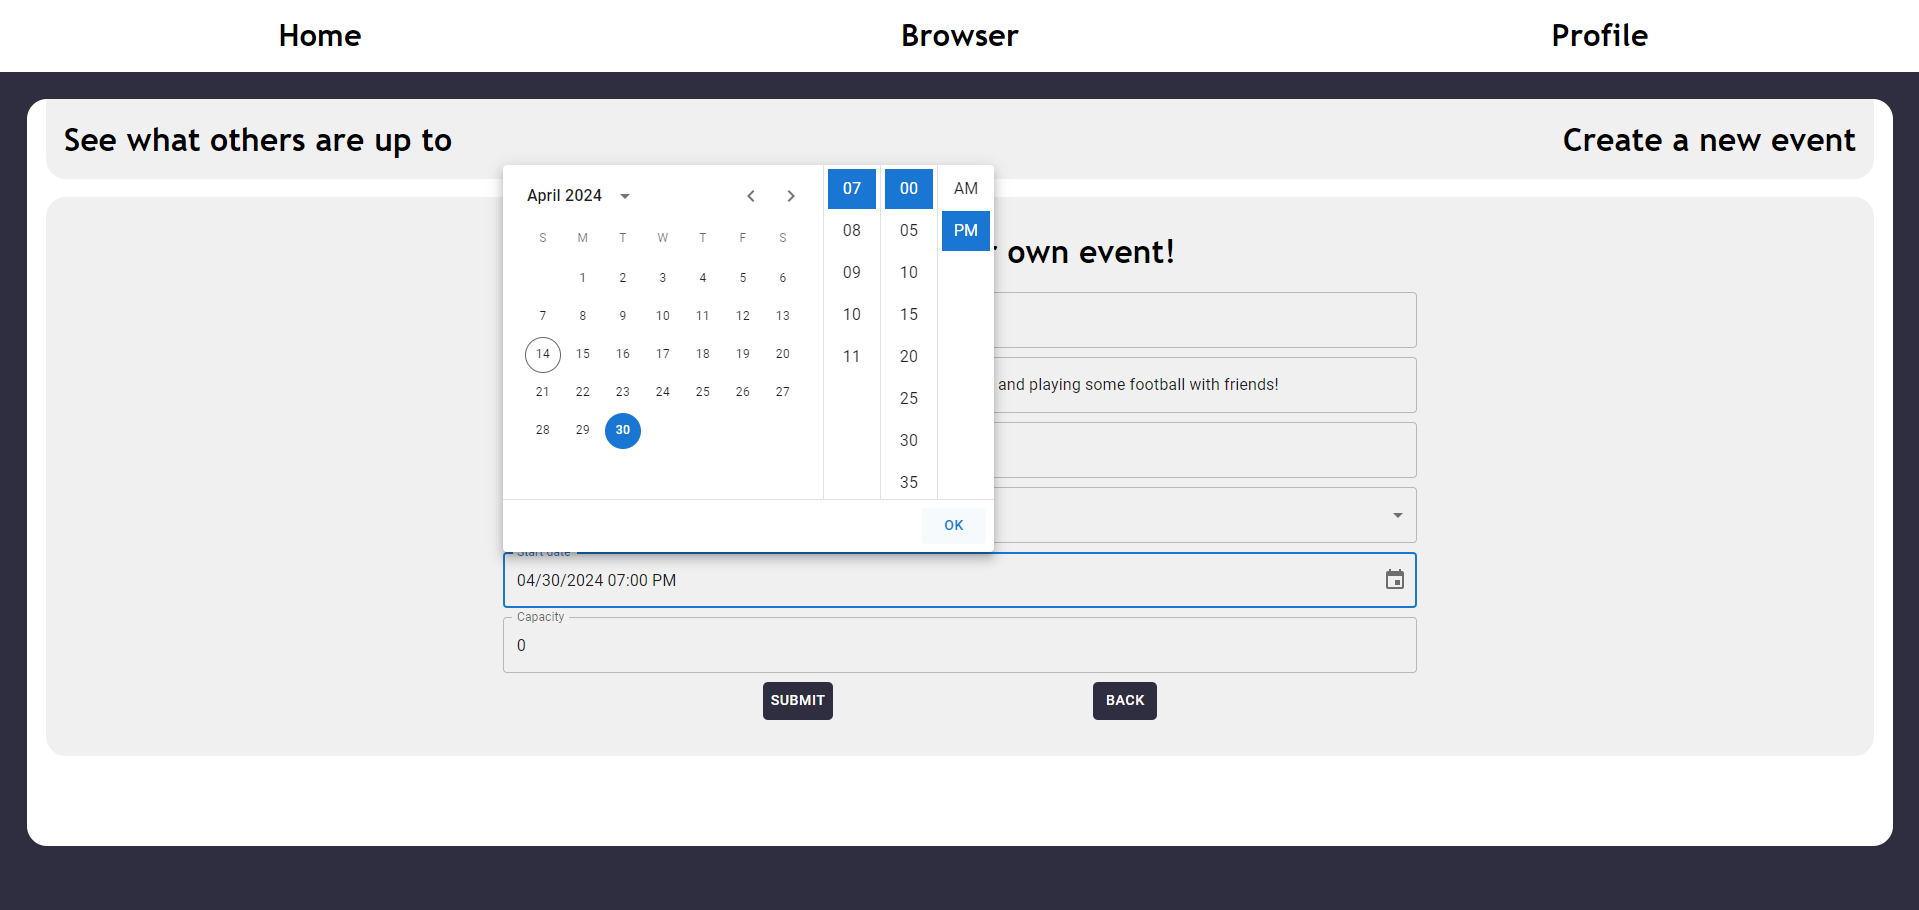
\includegraphics[width=0.5\textwidth]{images/create_event_3.png}
	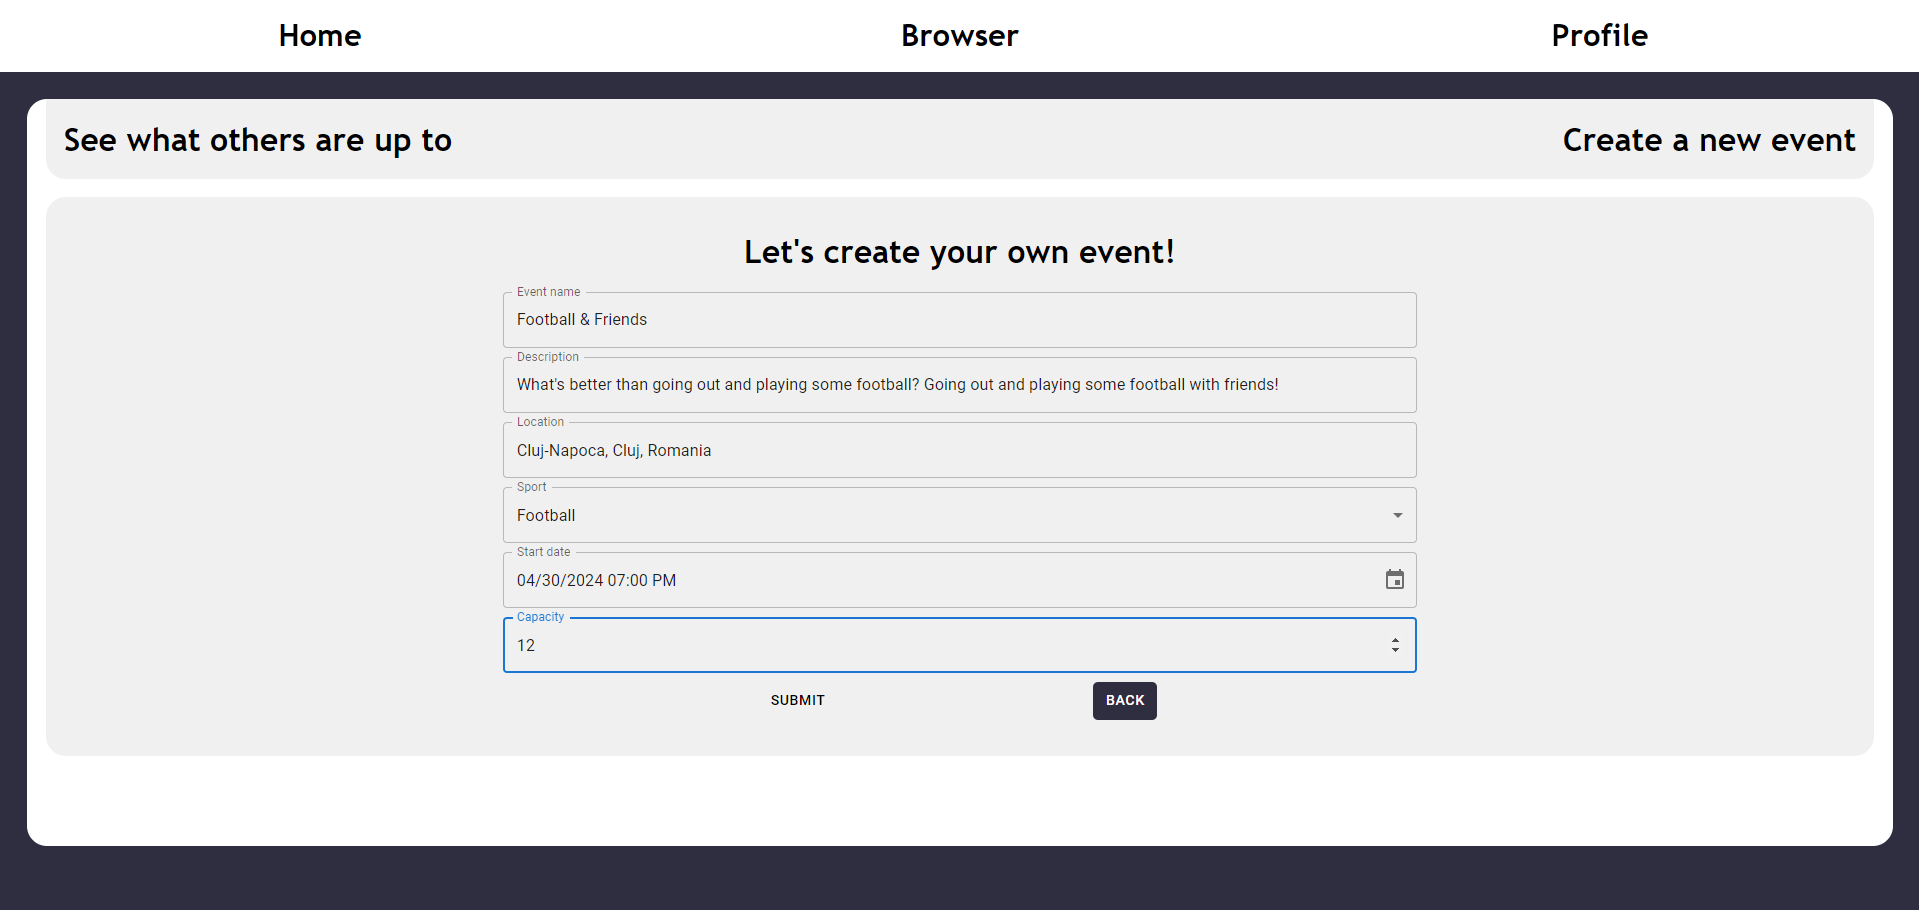
\includegraphics[width=0.5\textwidth]{images/create_event_4.png}
	\caption{Esemény létrehozása}
	\label{fig:create_event}
\end{figure}

\newpage

\begin{figure}[ht]
	\centering
	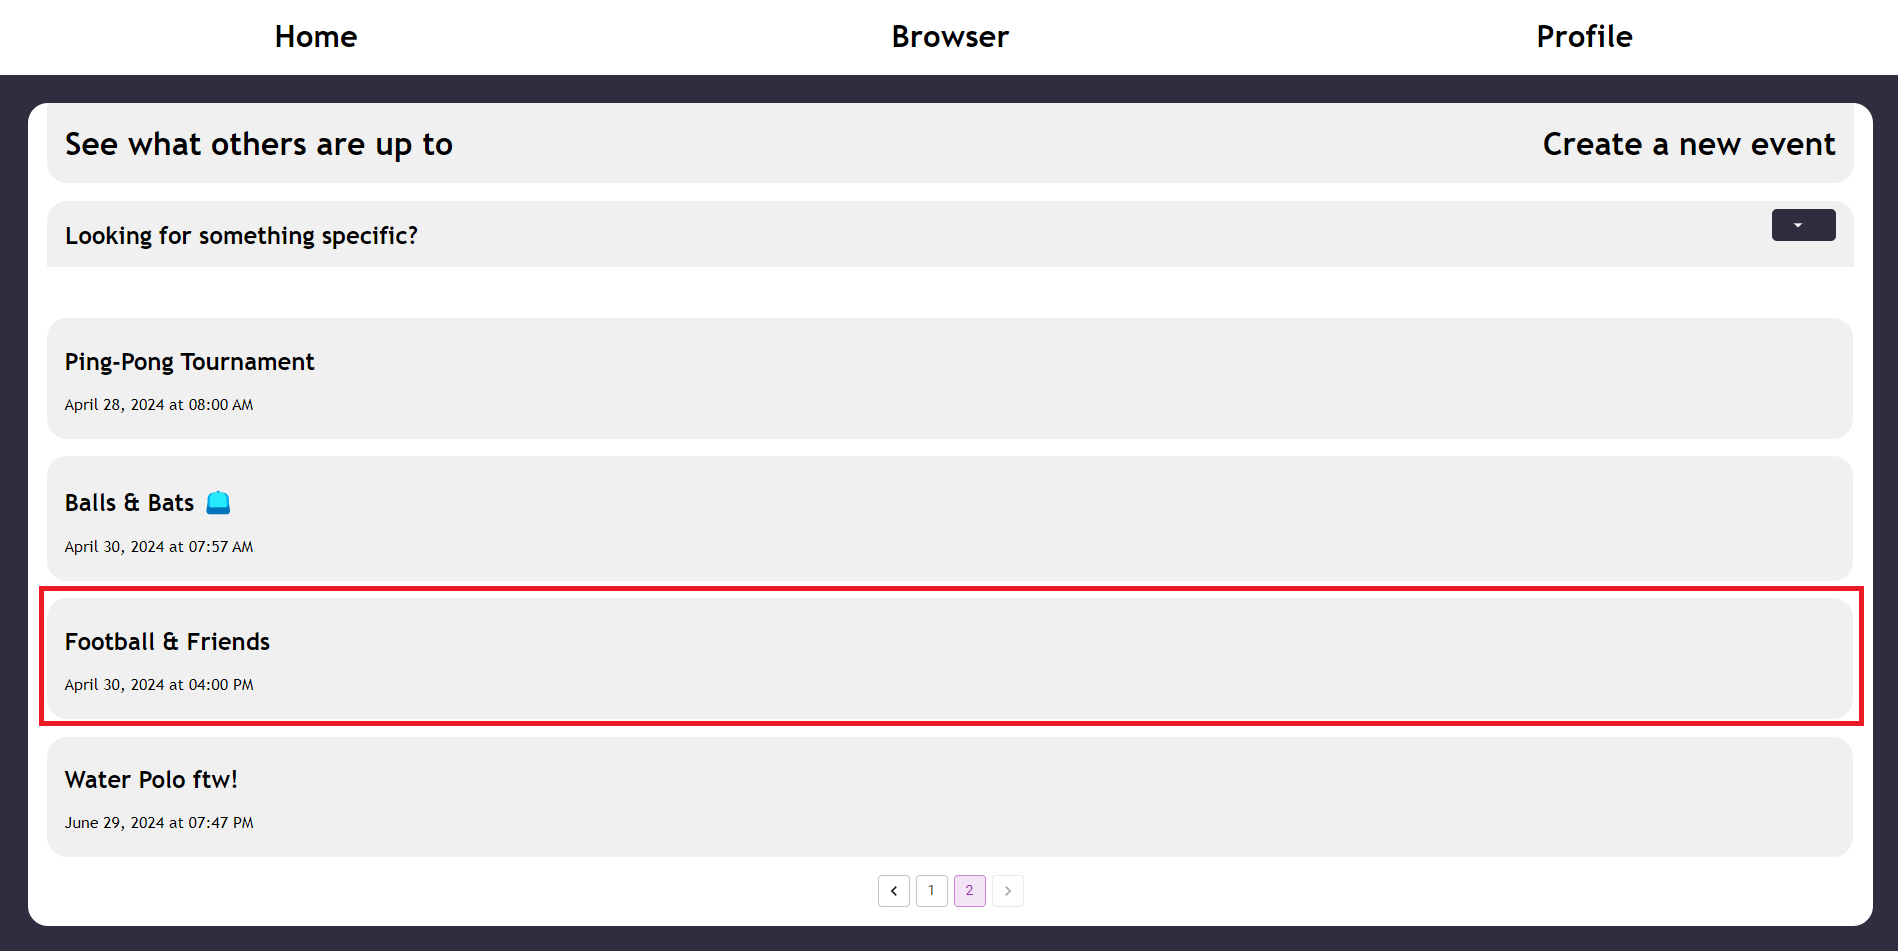
\includegraphics[width=0.7\textwidth]{images/new_event_created.png}
	\caption{Az újonnan létrehozott esemény a sportesemény böngészőben}
	\label{fig:new_event_created}
\end{figure}

Az esemény részletes megjelenítésében látható minden általunk megadott információt. Az eseméy azt is mutatja, hogy ki az esemény szervezője. A szerző nevére
kattitnva megtekinthető egy rövid leírás a szervező profiljáról. Ez látható a \ref{fig:event_creator}-es ábrán is.

\begin{figure}[h]
	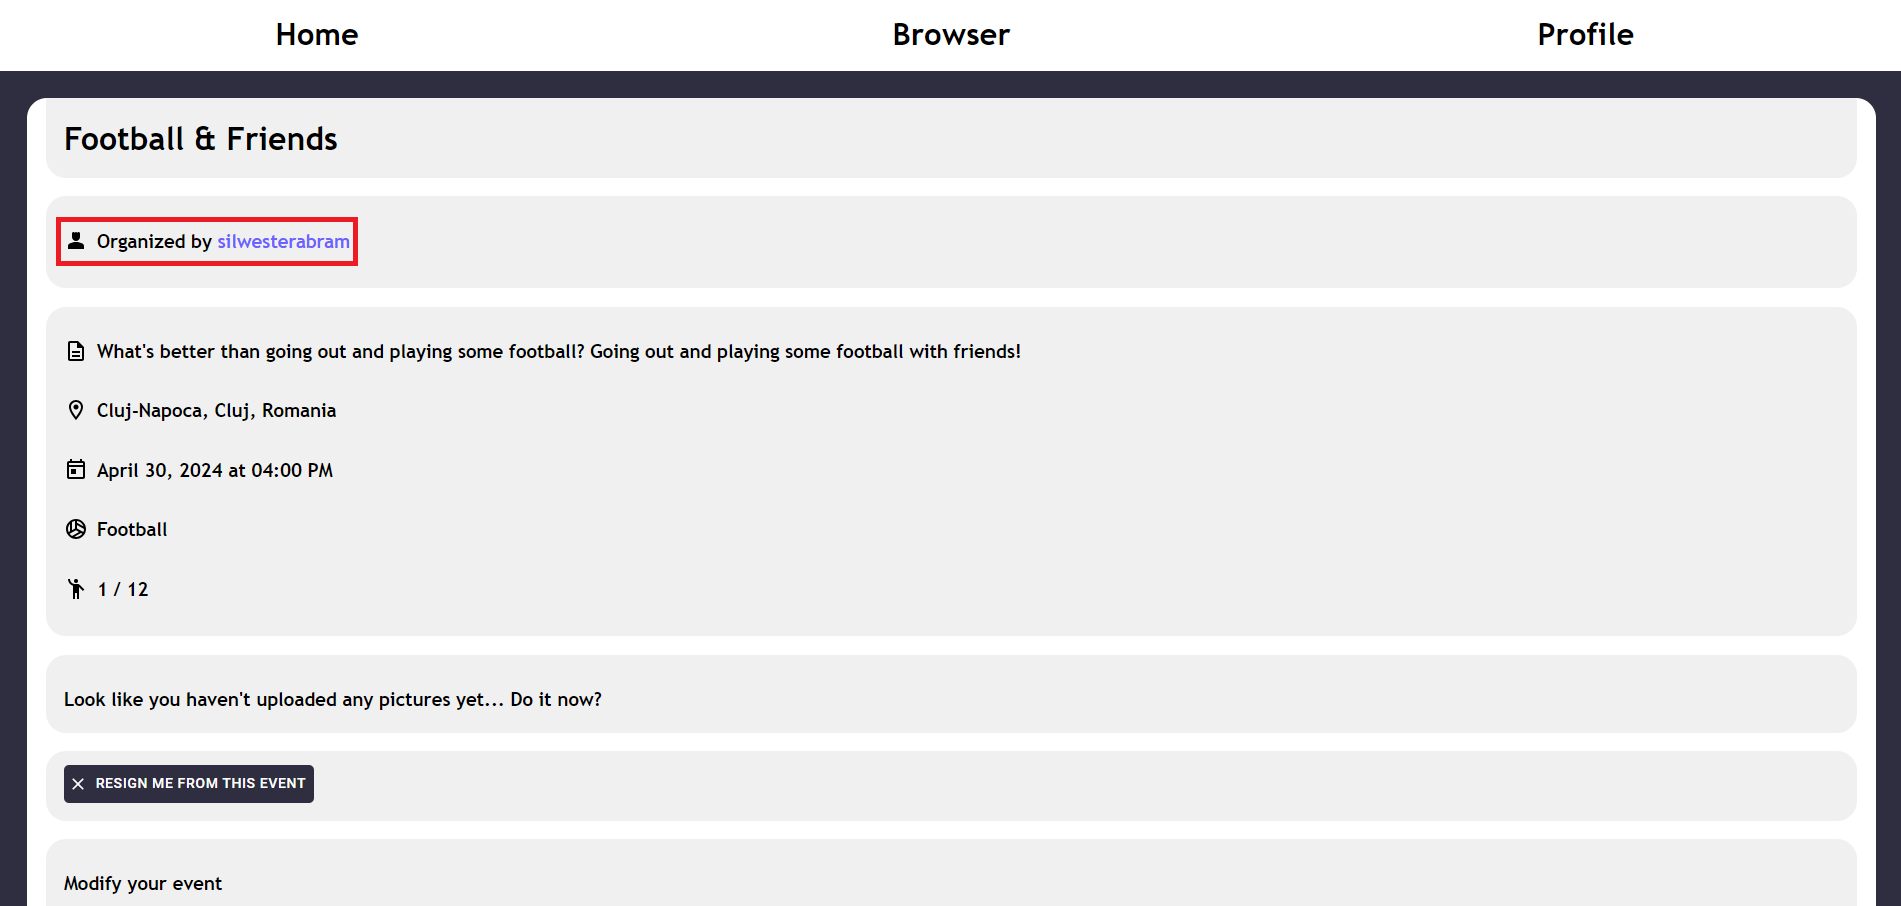
\includegraphics[width=0.5\textwidth]{images/sports_event_creator.png}
	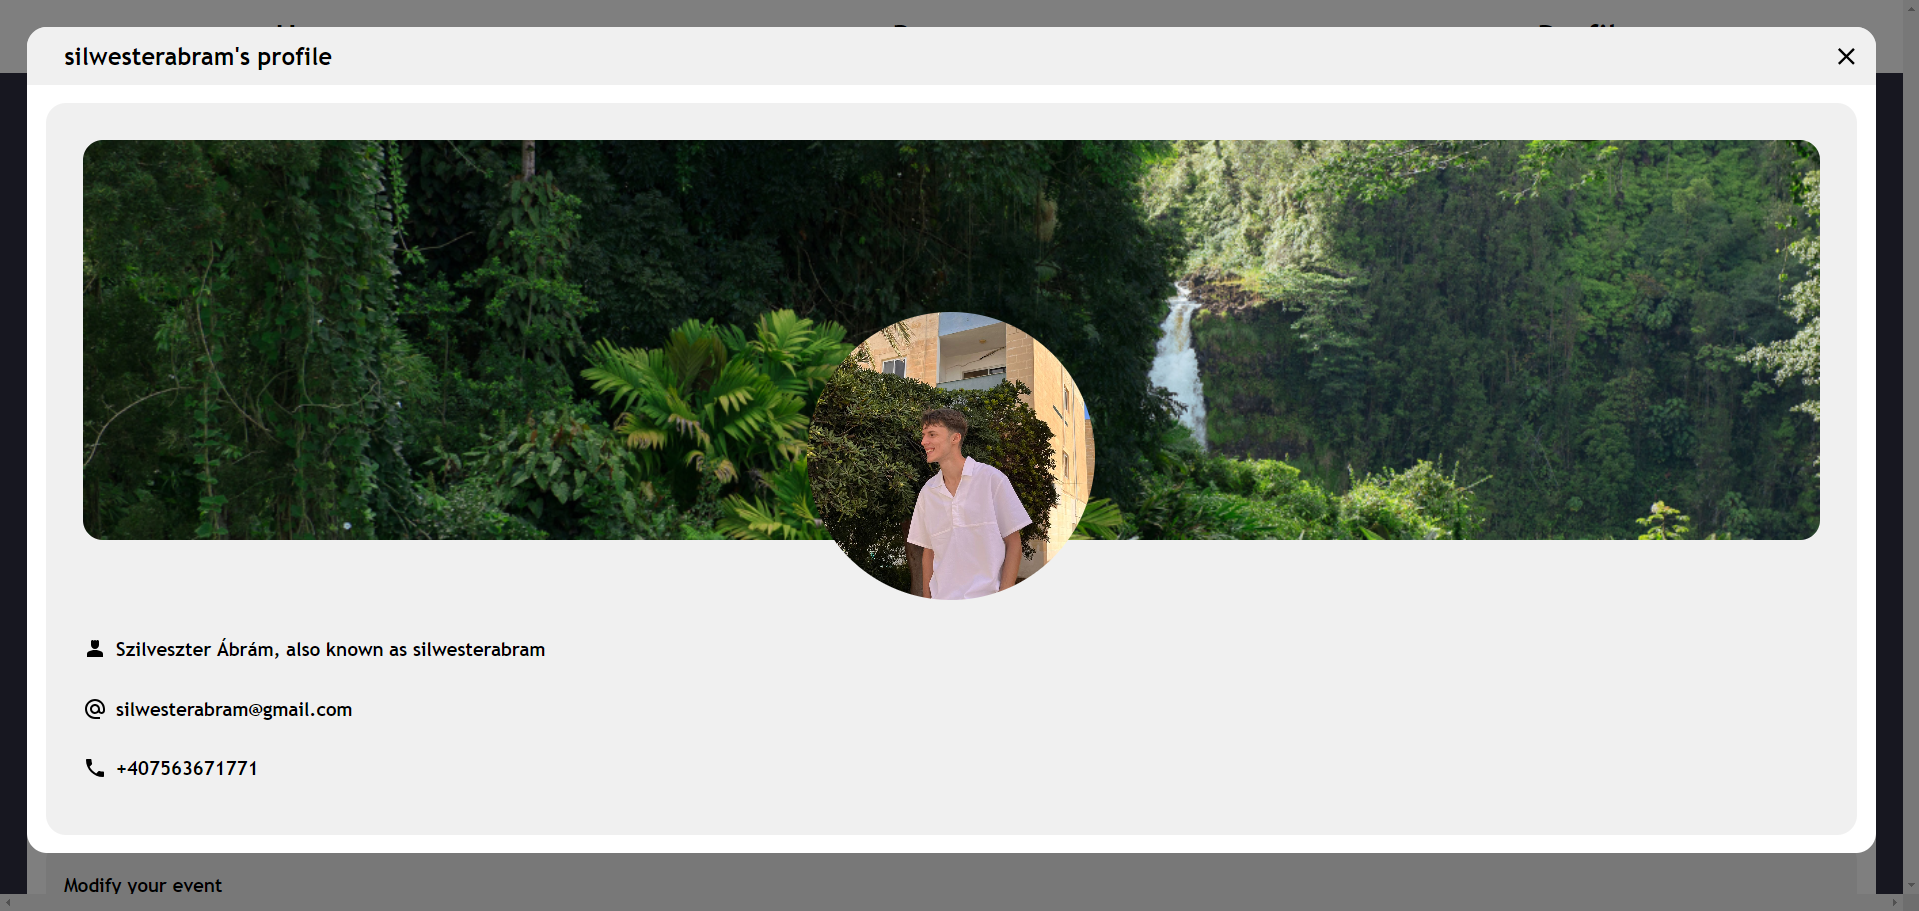
\includegraphics[width=0.5\textwidth]{images/sports_event_creator_profile_view.png}
	\caption{Az esemény szervezőjének megjelenítése}
	\label{fig:event_creator}
\end{figure}

Egy esemény létrehozásakor az esemény szervezője automatikusan feliratkozik erre. Amennyiben ezt vissza szeretné vonni, a
``Resign me from this event'' gomb segítségével megteheti. Ilyenkor megfigyelhető, hogy az eseményre jelentkezett egyének száma egyel csökken.
Ez megfigyelhető a \ref{fig:resign_from_event}-es ábrán.

\begin{figure}[h]
	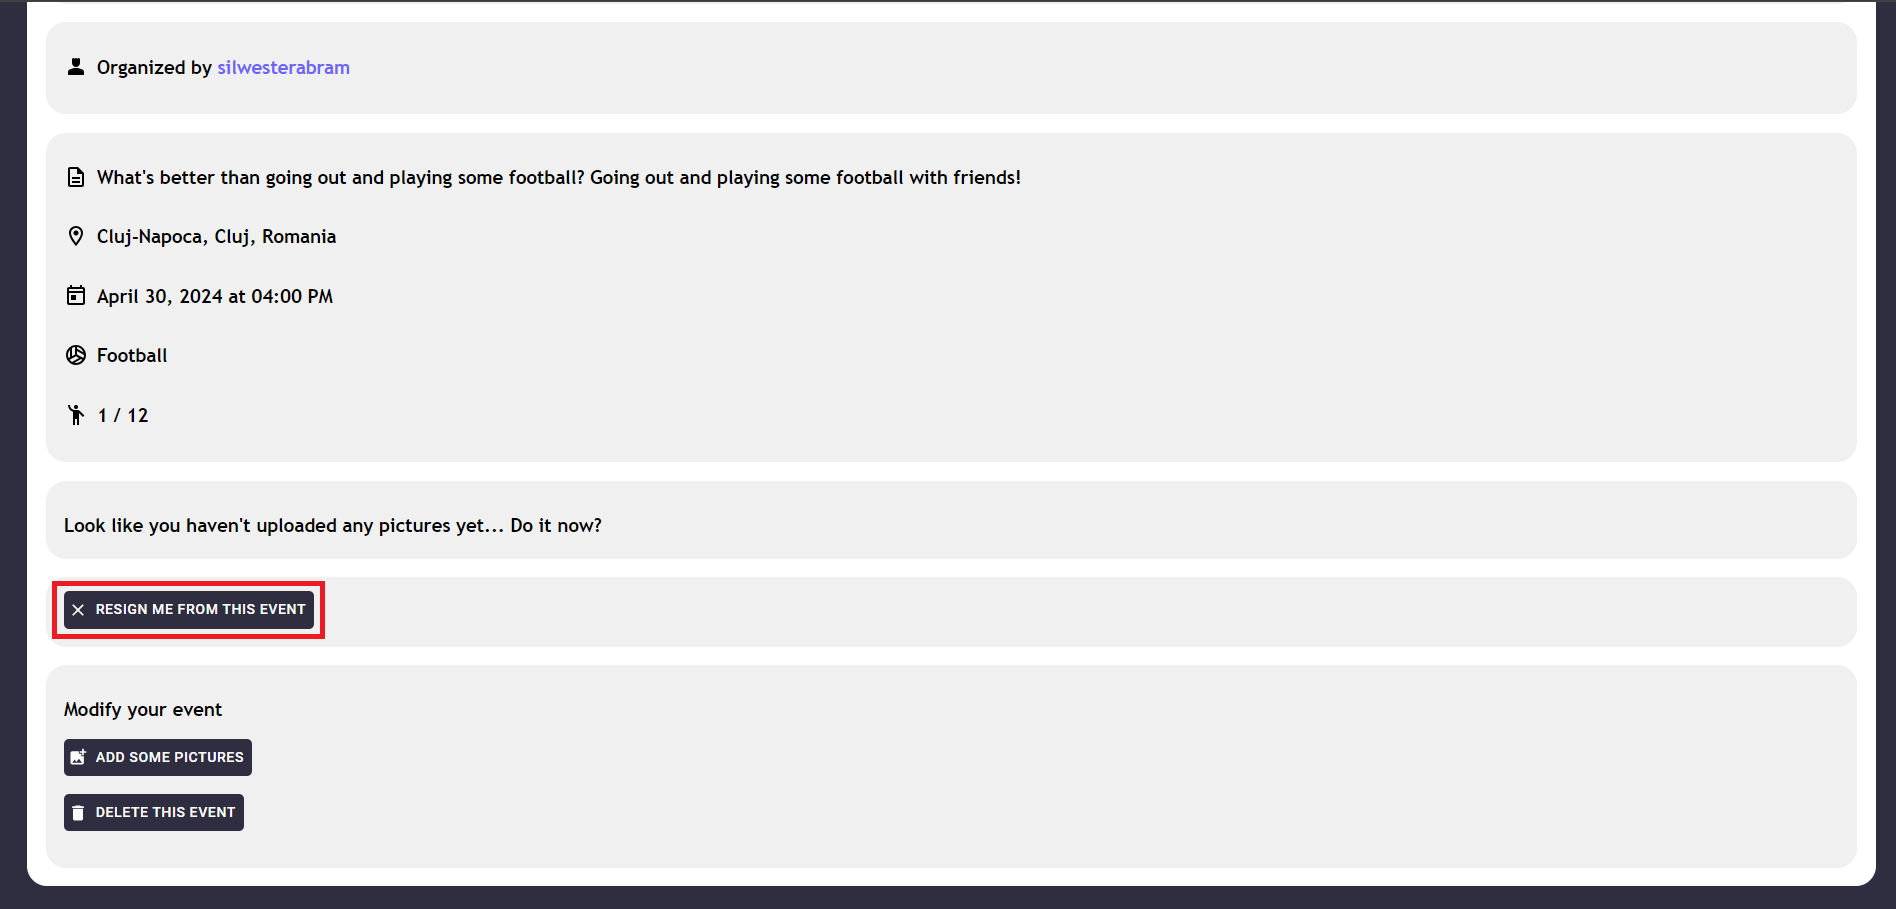
\includegraphics[width=0.5\textwidth]{images/resign_from_event_1.png}
	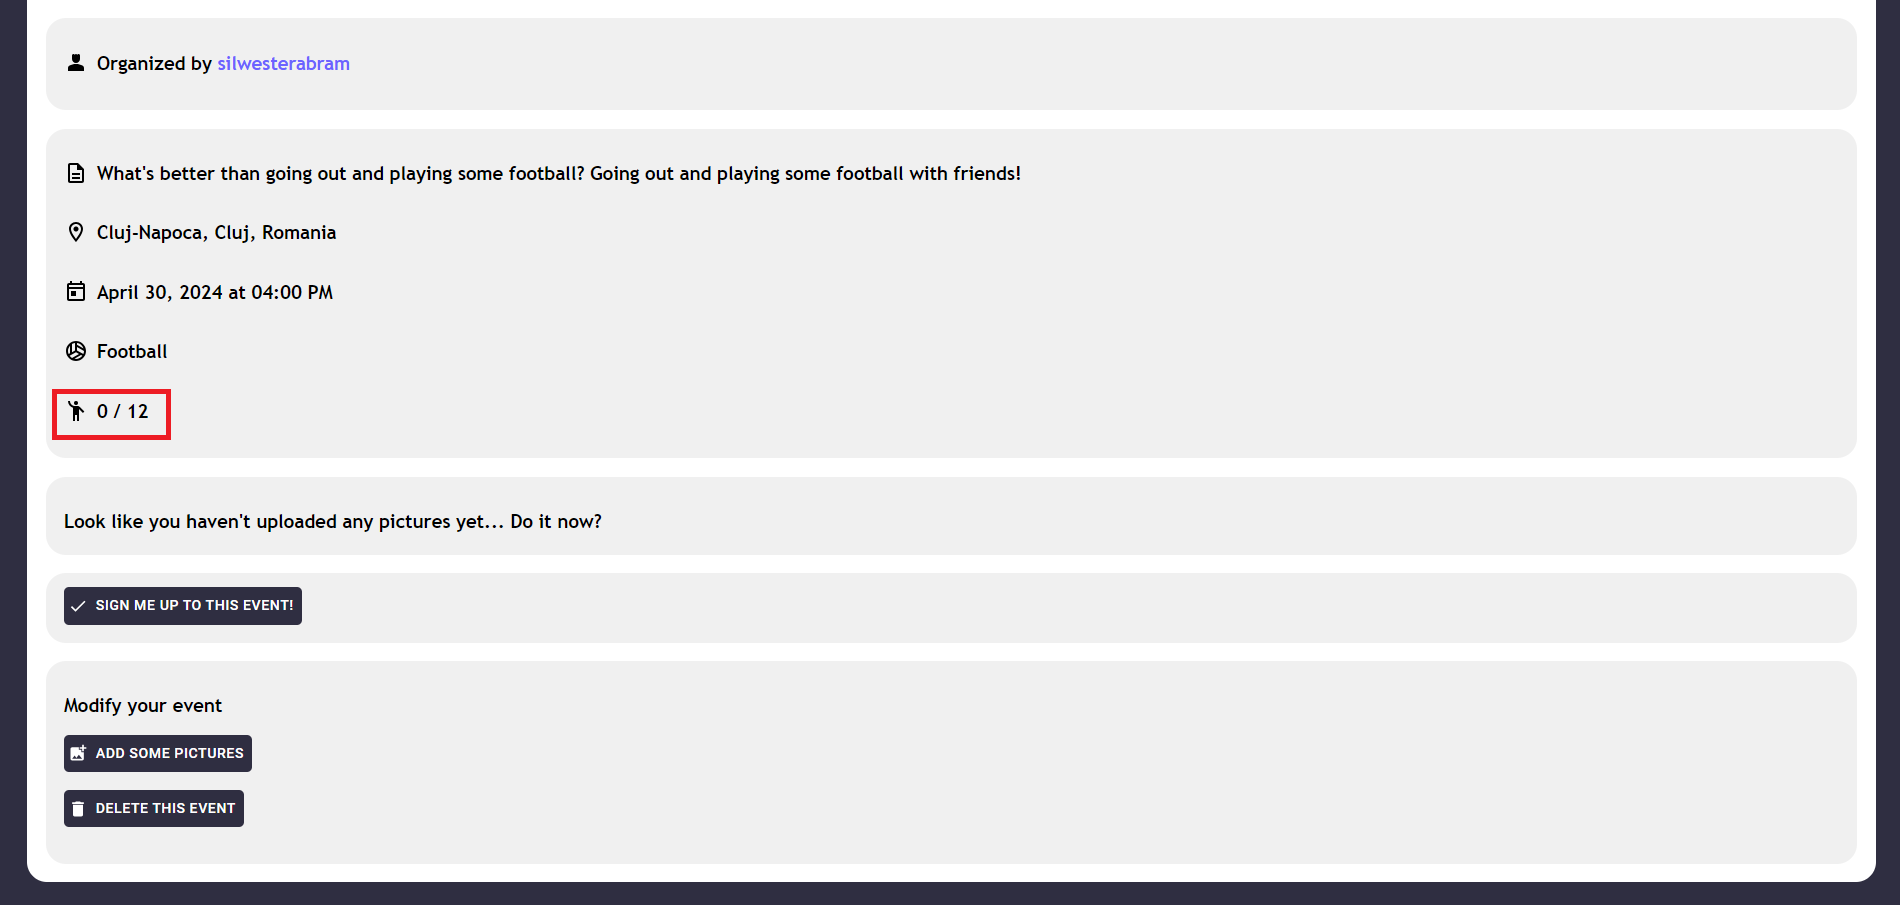
\includegraphics[width=0.5\textwidth]{images/resign_from_event_2.png}
	\caption{Egy eseményről való leiratkozás}
	\label{fig:resign_from_event}
\end{figure}

Szervezőként adhatunk hozzá képeket is az általunk szervezett eseményekhez. Ezt az ``Add some pictures'' gombra való kattintással tehetjük meg.
Ez felhoz egy ablakot, majd itt a képek kiválasztása után az oldal frissül és láthatóak lesznek az általunk kiválasztott képek. Ez a folyamat
látható a \ref{fig:add_pictures_event}-es ábrán.

\begin{figure}[ht]
	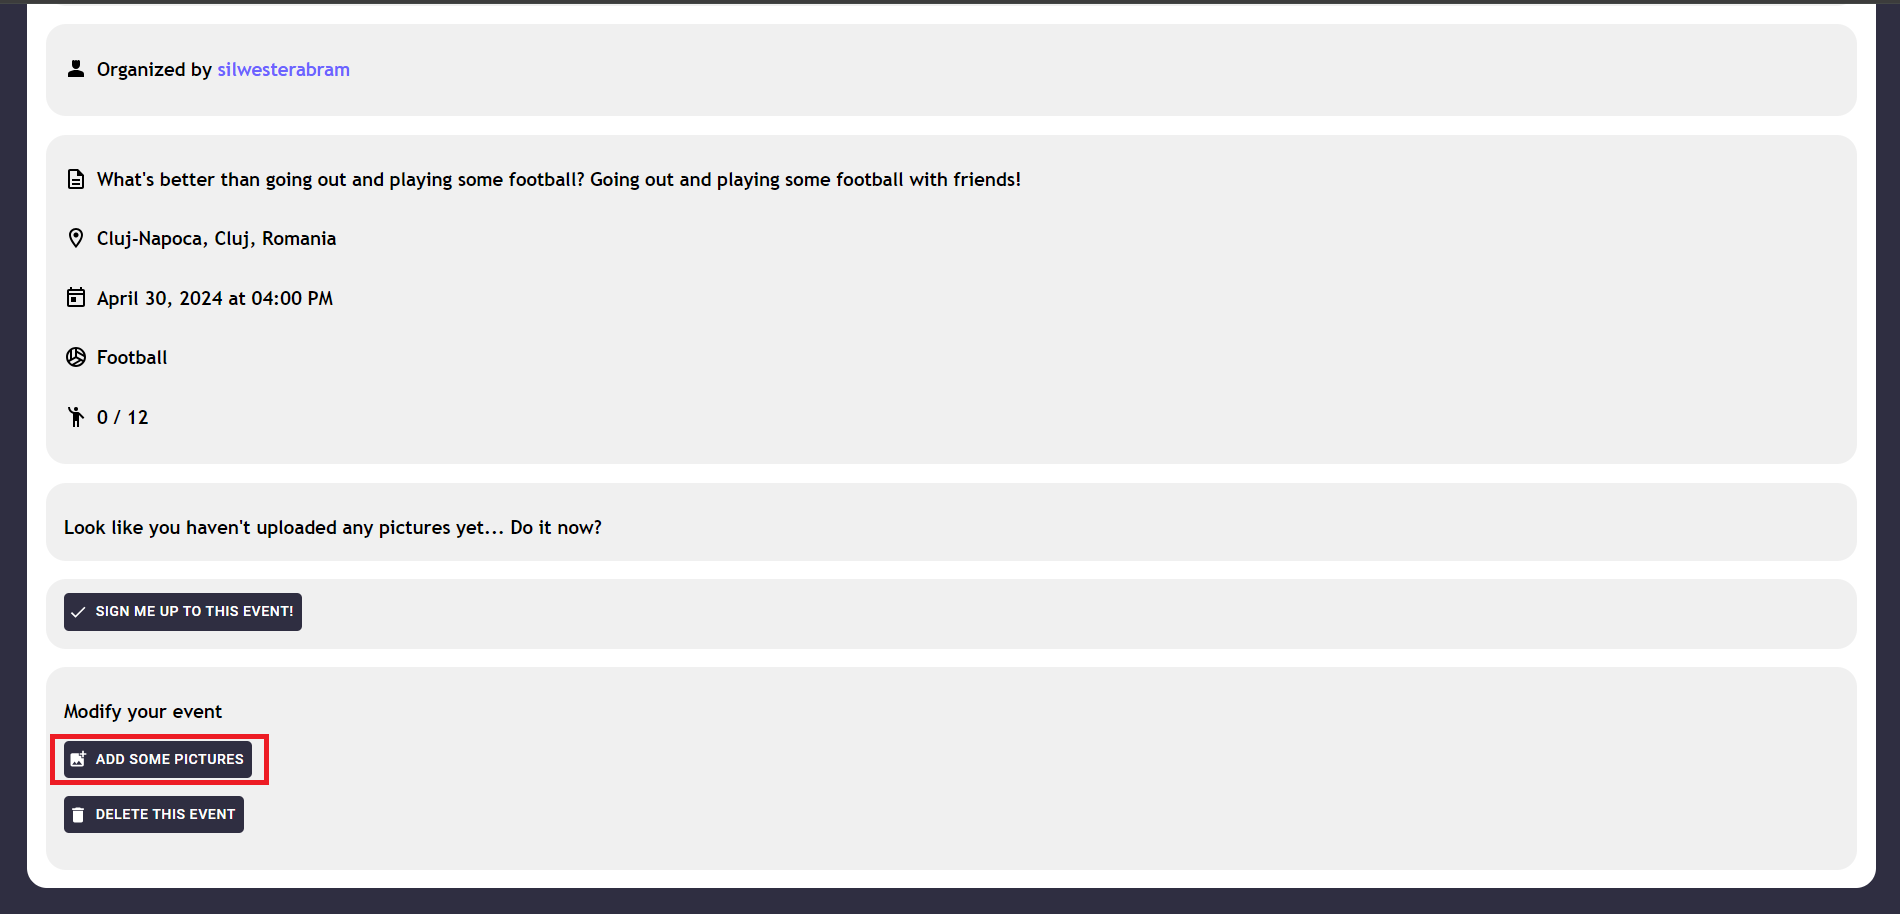
\includegraphics[width=0.5\textwidth]{images/add_pictures_event.png}
	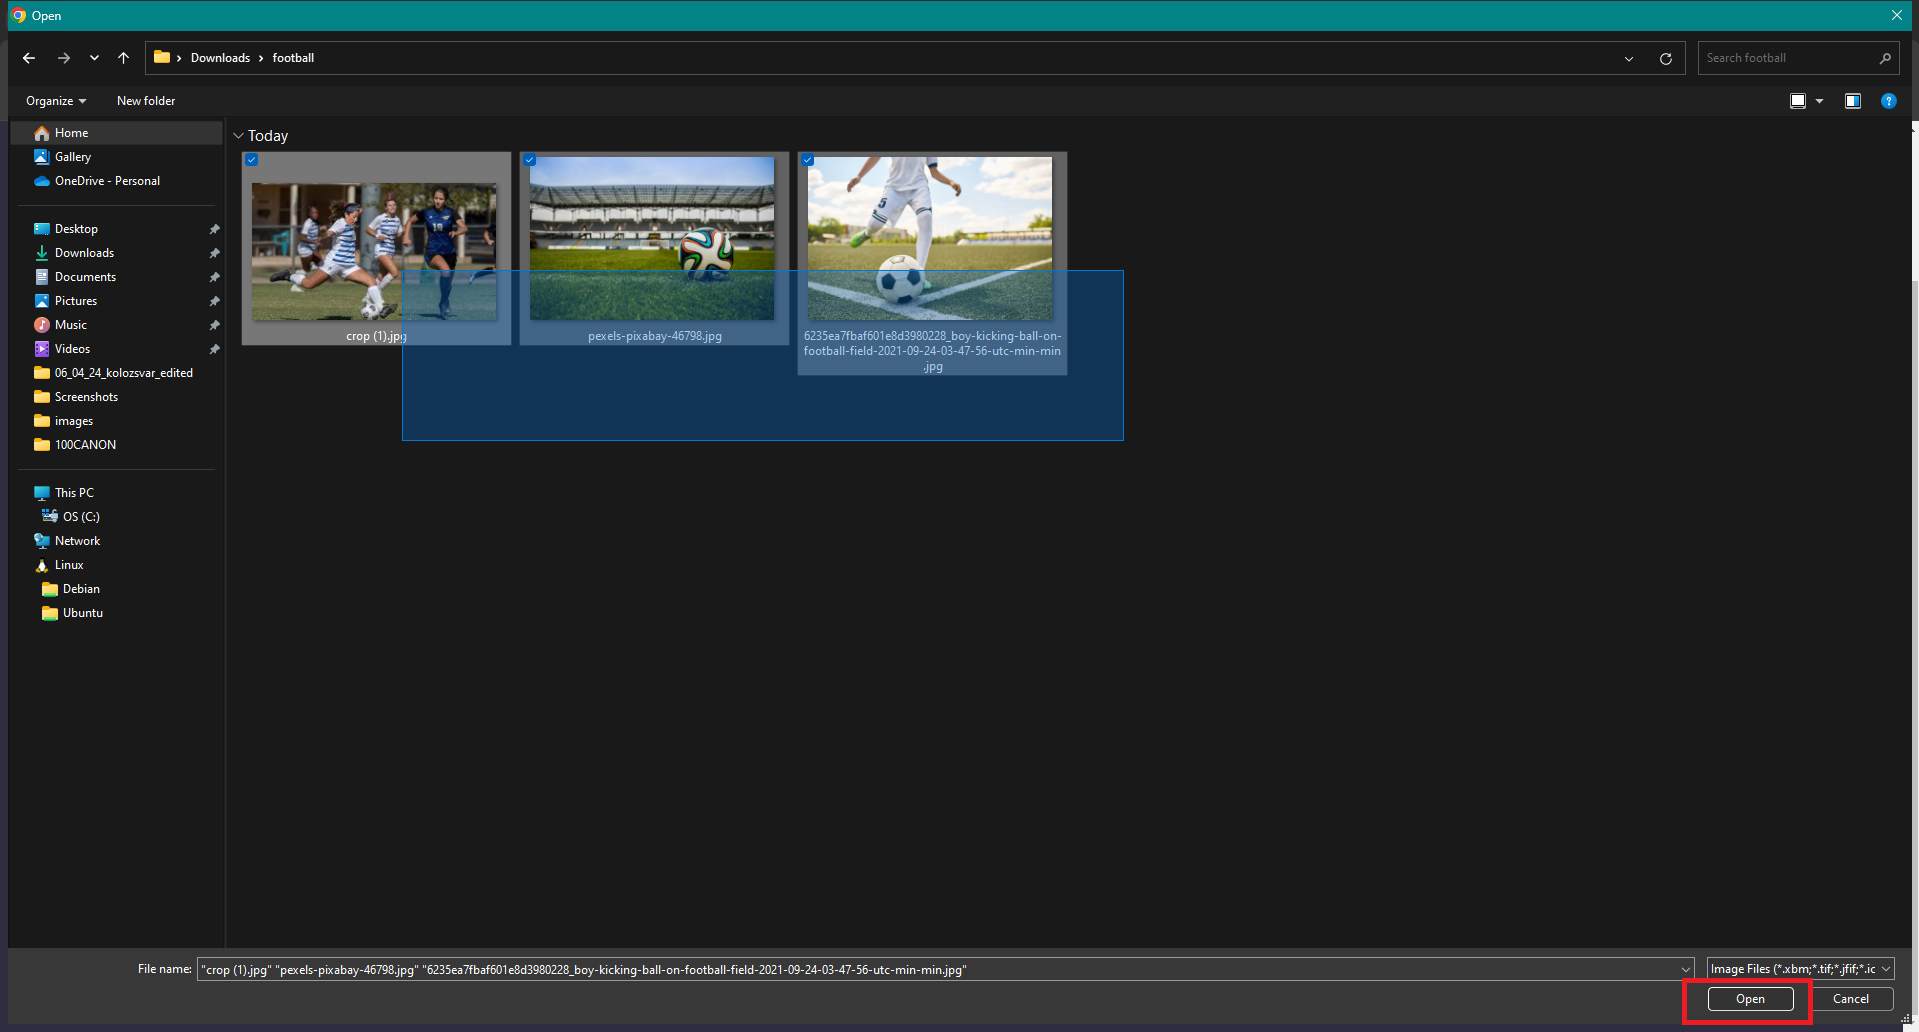
\includegraphics[width=0.5\textwidth]{images/add_pictures_event_2.png}
	\begin{center}
		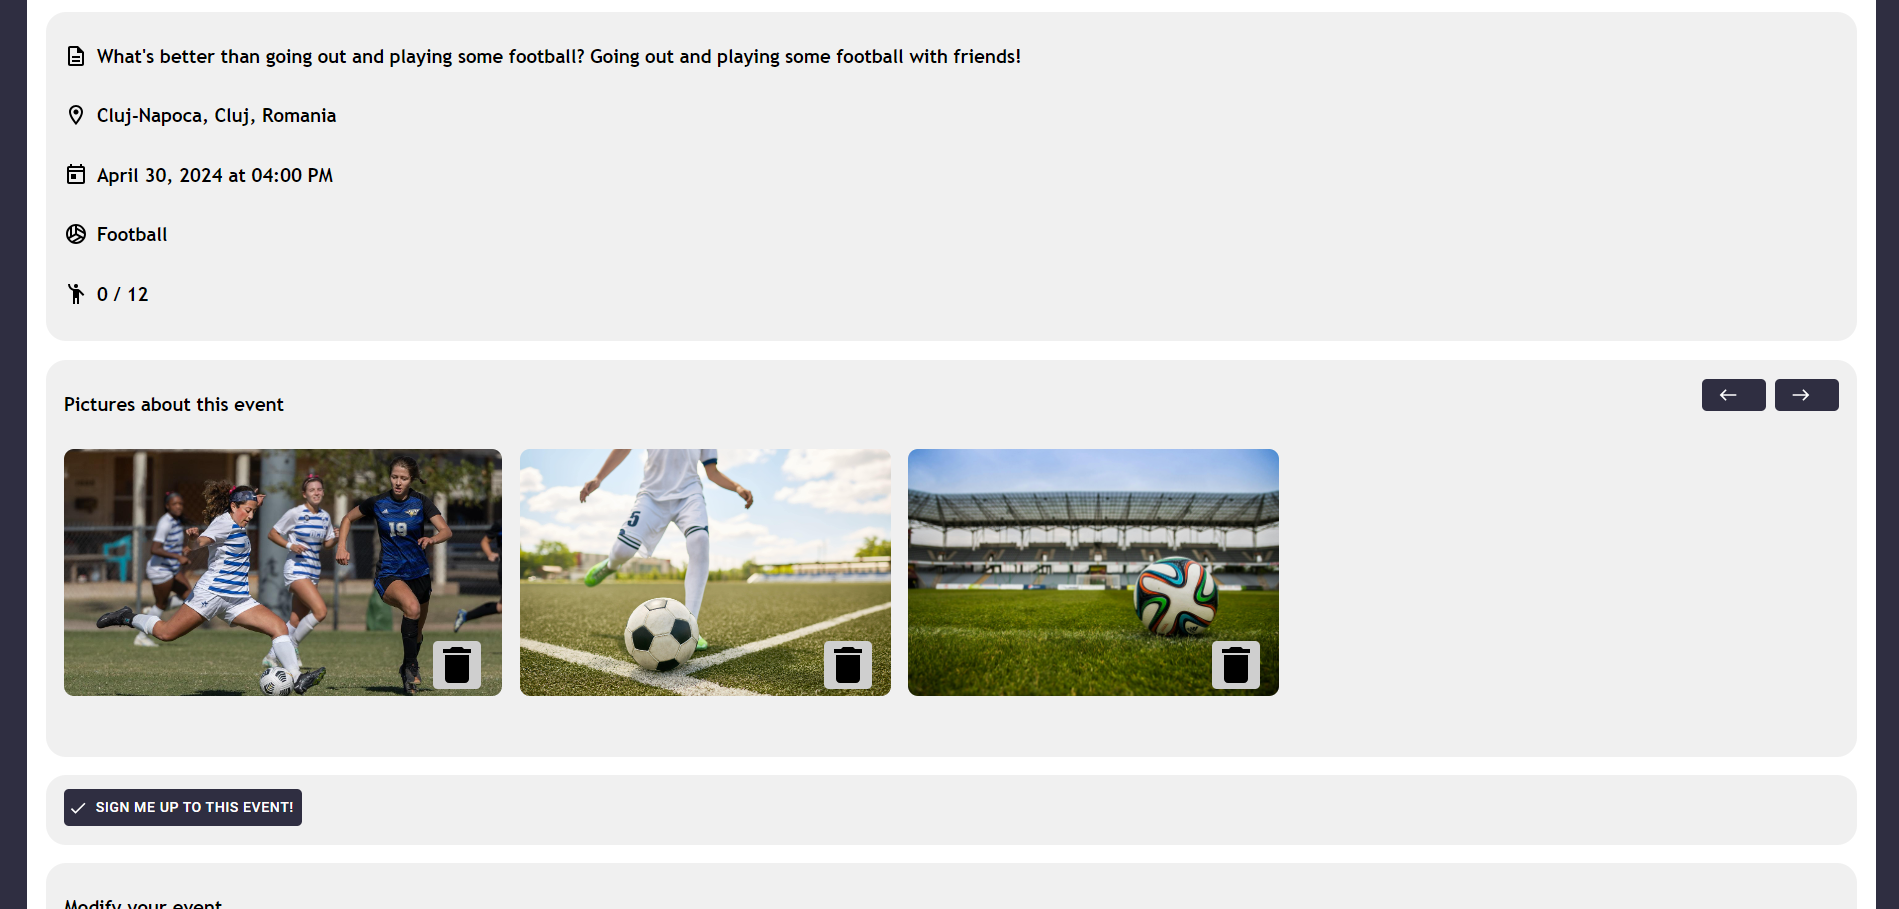
\includegraphics[width=0.7\textwidth]{images/add_pictures_event_3.png}
	\end{center}
	\caption{Képek hozzáadása az eseményhez}
	\label{fig:add_pictures_event}
\end{figure}

Egy esemény szervezője törölhet is képeket az eseményről. Ezt a kép jobb alsó sarkában megjelenő törlés ikonra kattintással teheti meg. Ilyenkor az oldal 
tartalma automatikusan frissül, s a törölni kívánt kép eltűnik az esemény oldaláról. Ez megfigyelhető a \ref{fig:delete_image_event}-as ábrán.

\begin{figure}[h]
	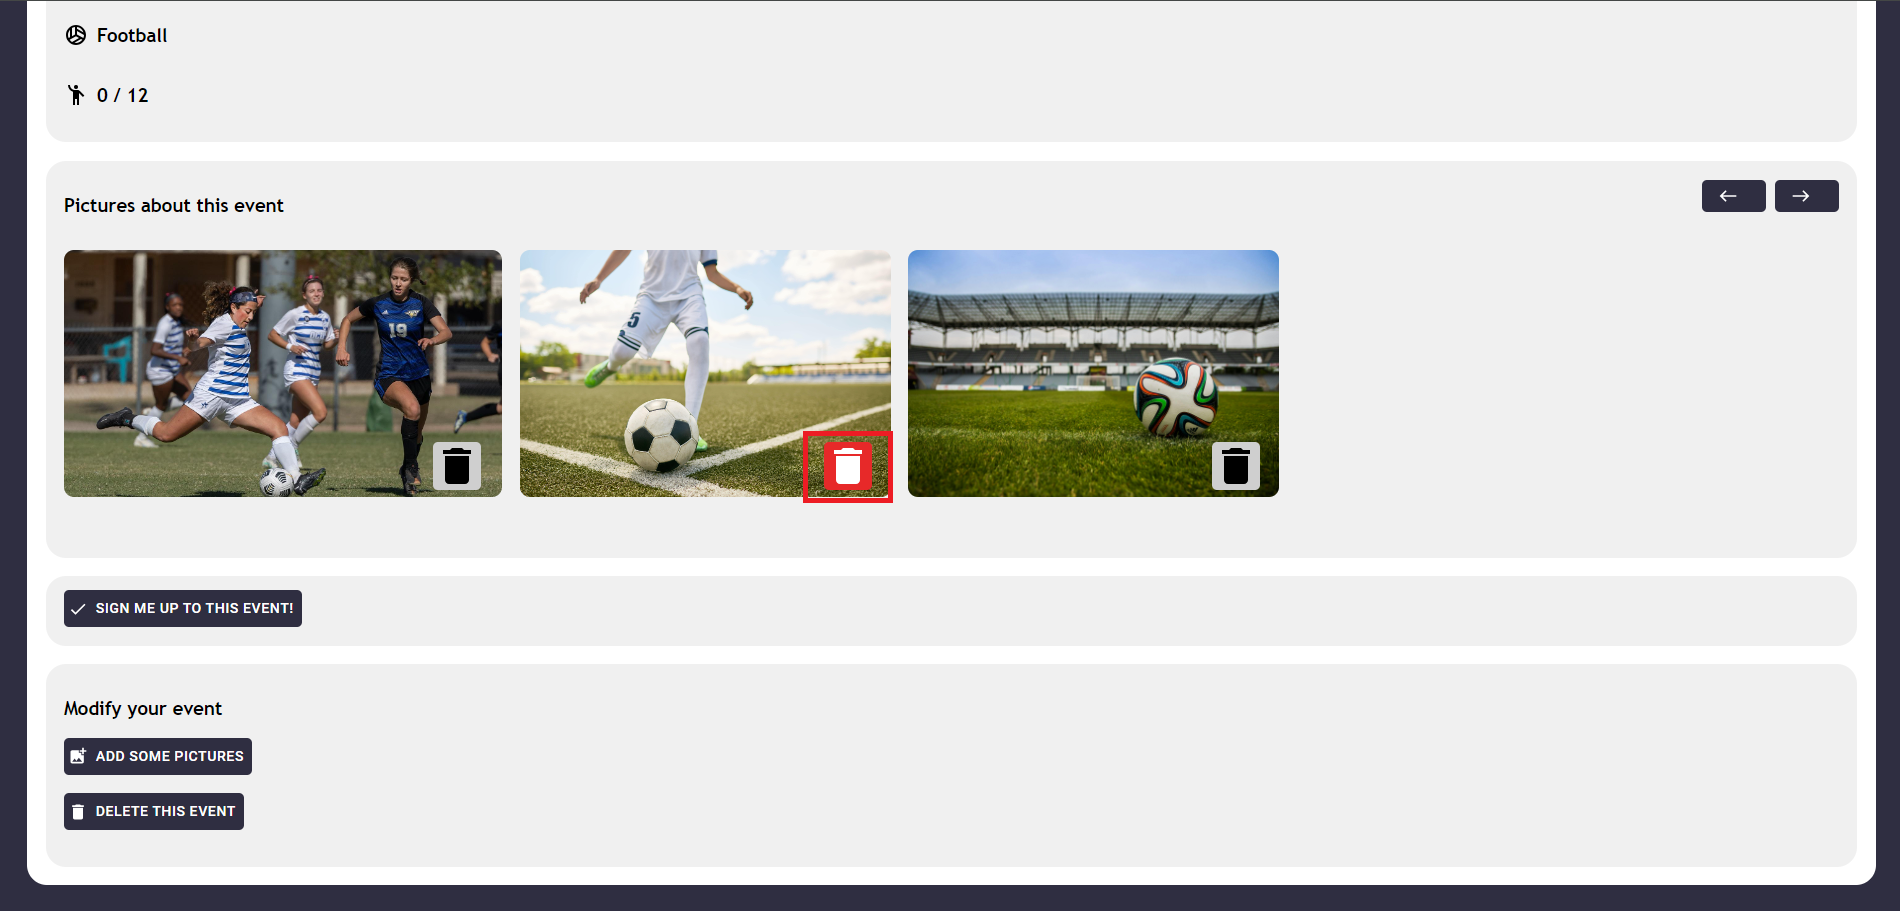
\includegraphics[width=0.5\textwidth]{images/delete_image_event_1.png}
	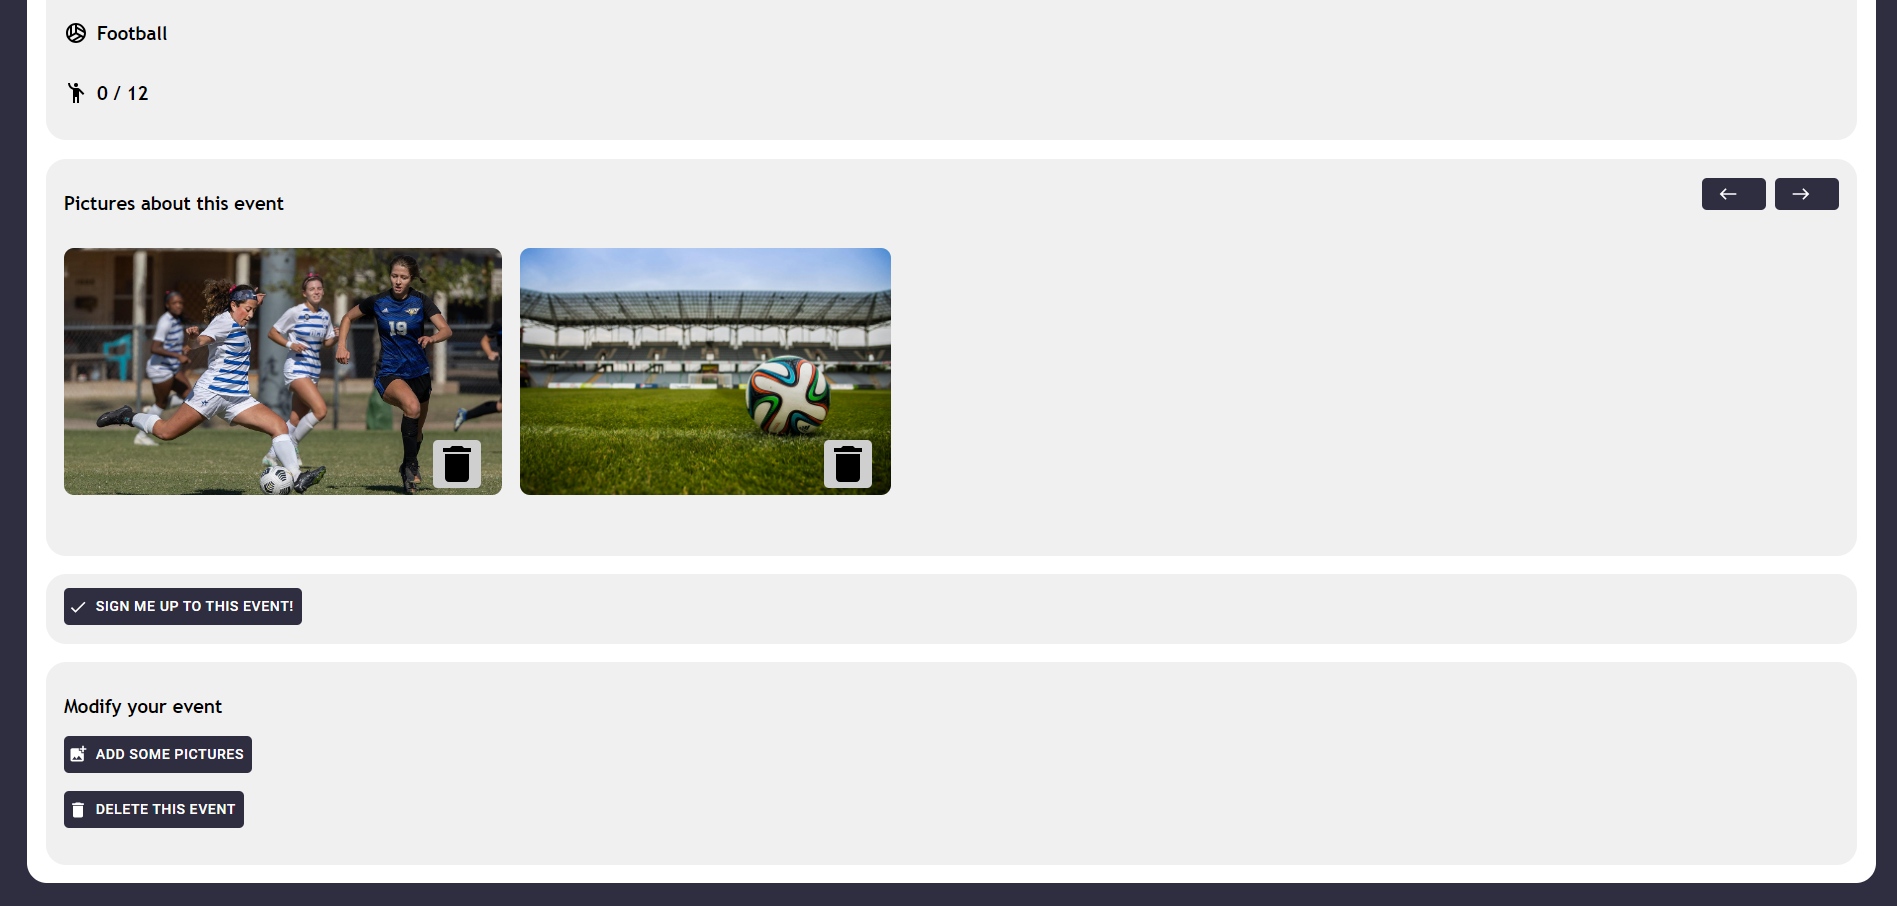
\includegraphics[width=0.5\textwidth]{images/delete_image_event_2.png}
	\caption{Kép törlése az eseményről}
	\label{fig:delete_image_event}
\end{figure}

Végső soron a szervező törölheti is az általa szervezett eseményt. Ezt a ``Delete this event'' gombra való kattintással teheti meg, ahogyan a \ref{fig:delete_event_details}-es ábrán is látható.
Ilyenkor egy megerősítendő ablak jelenik meg, amiben ha a ``Yes, delete this event!'' gombra kattintunk, az esemény véglegesen törlése kerül.
Ezután az oldal átirányít bennünket a böngésző felületre, ahol már nem fogjuk látni az általunk törölt eseményt.

\newpage

\begin{figure}[ht]
	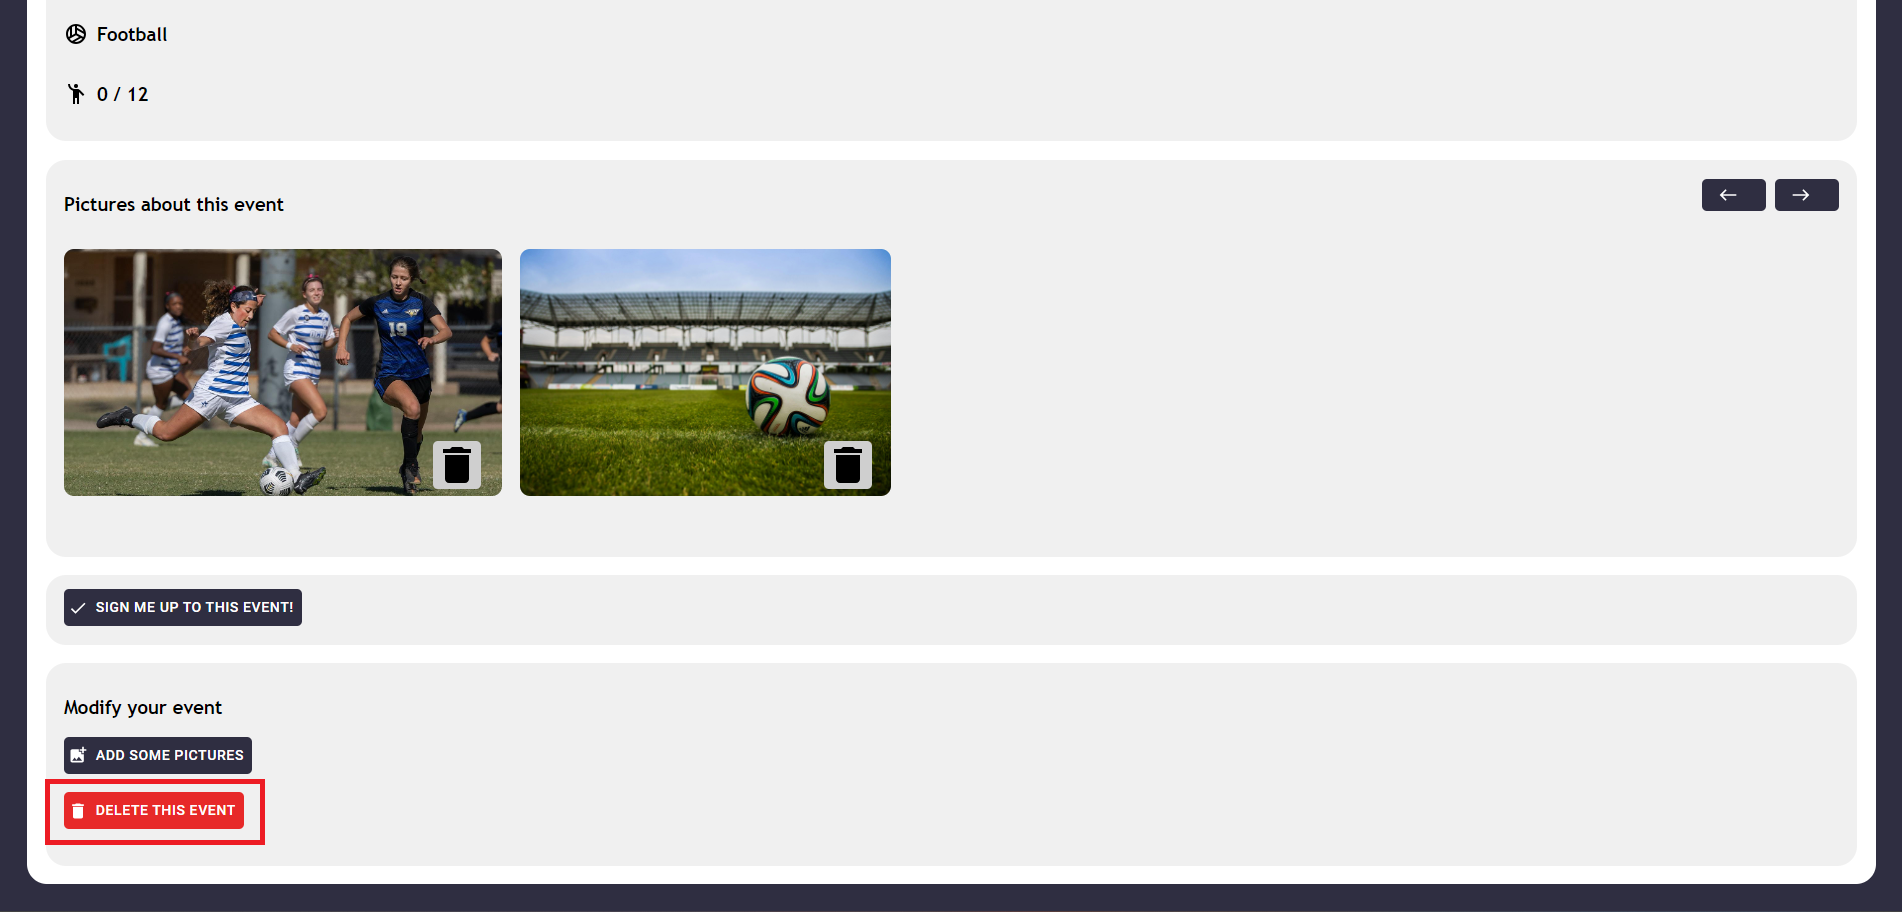
\includegraphics[width=0.5\textwidth]{images/delete_this_event_1.png}
	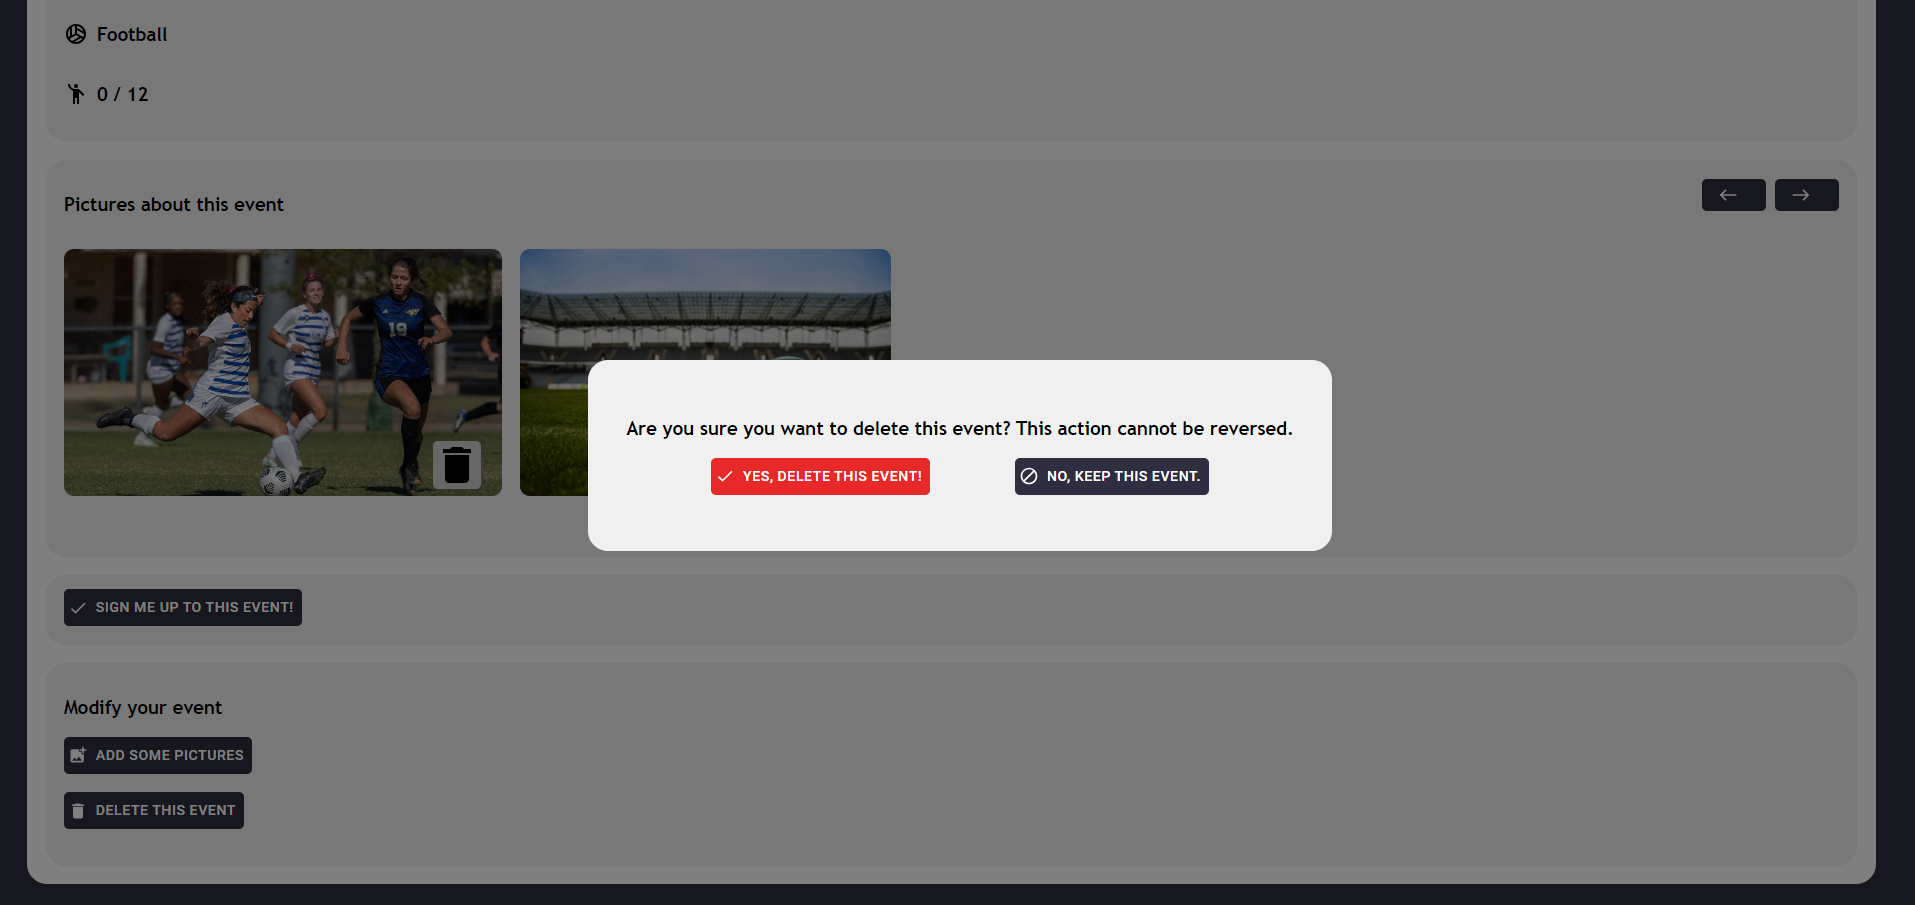
\includegraphics[width=0.5\textwidth]{images/delete_this_event_2.png}
	\caption{Esemény törlése}
	\label{fig:delete_event_details}
\end{figure}

\subsection{Sportesemények szűrése}

A sportesemények böngészése során a felhasználónak lehetősége van kölünböző szűrők használatára.
A szűrők segítségével meg lehet határozni egy időintervallumot, amely alatt az eseményeket meg szeretnénk tekinteni, illetve kiválasztható egy
specifikus sport is, amely alapján lehetősége van a felhasználóknak szűrni az eseményeket.

A szűrők használatához előszőr kattintsunk a ``Looking for something specific?'' fülre:

\begin{figure}[h]
	\centering
	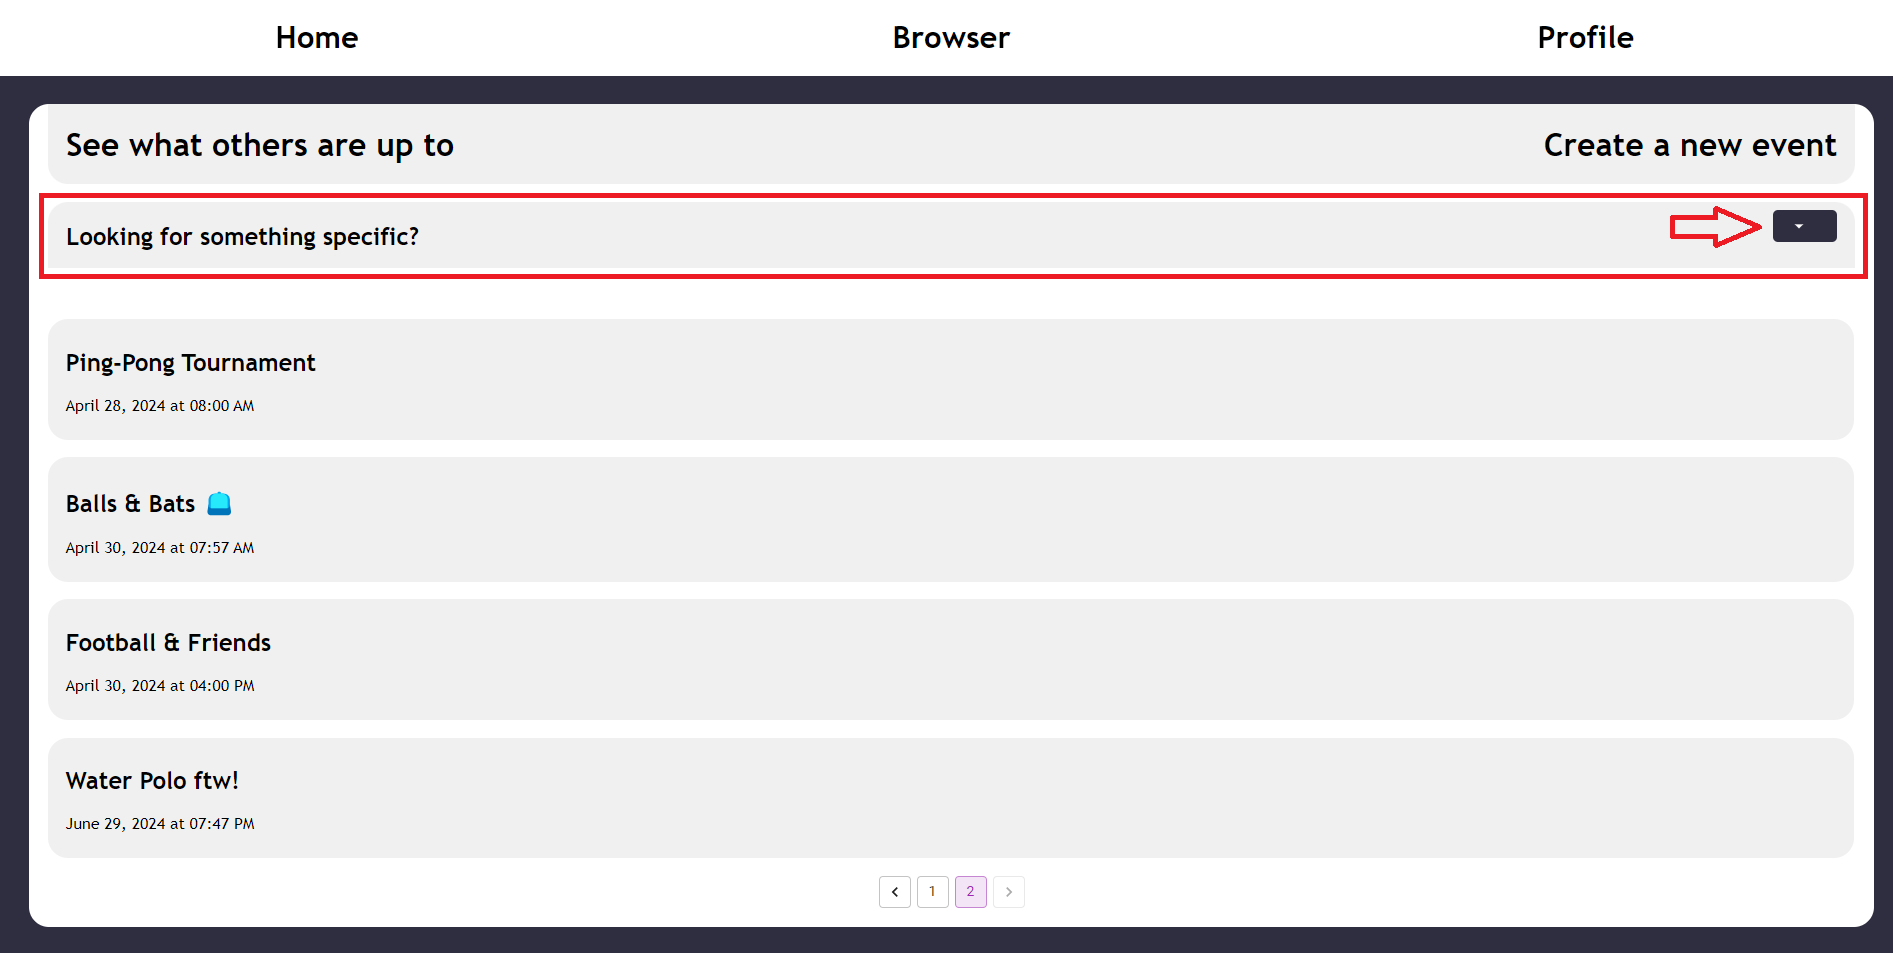
\includegraphics[width=0.5\textwidth]{images/filtering_events_1.png}
	\caption{A szűrőket tartalmazó fül előhozása}
	\label{fig:filter_1}
\end{figure}

\newpage

\begin{figure}[ht]
	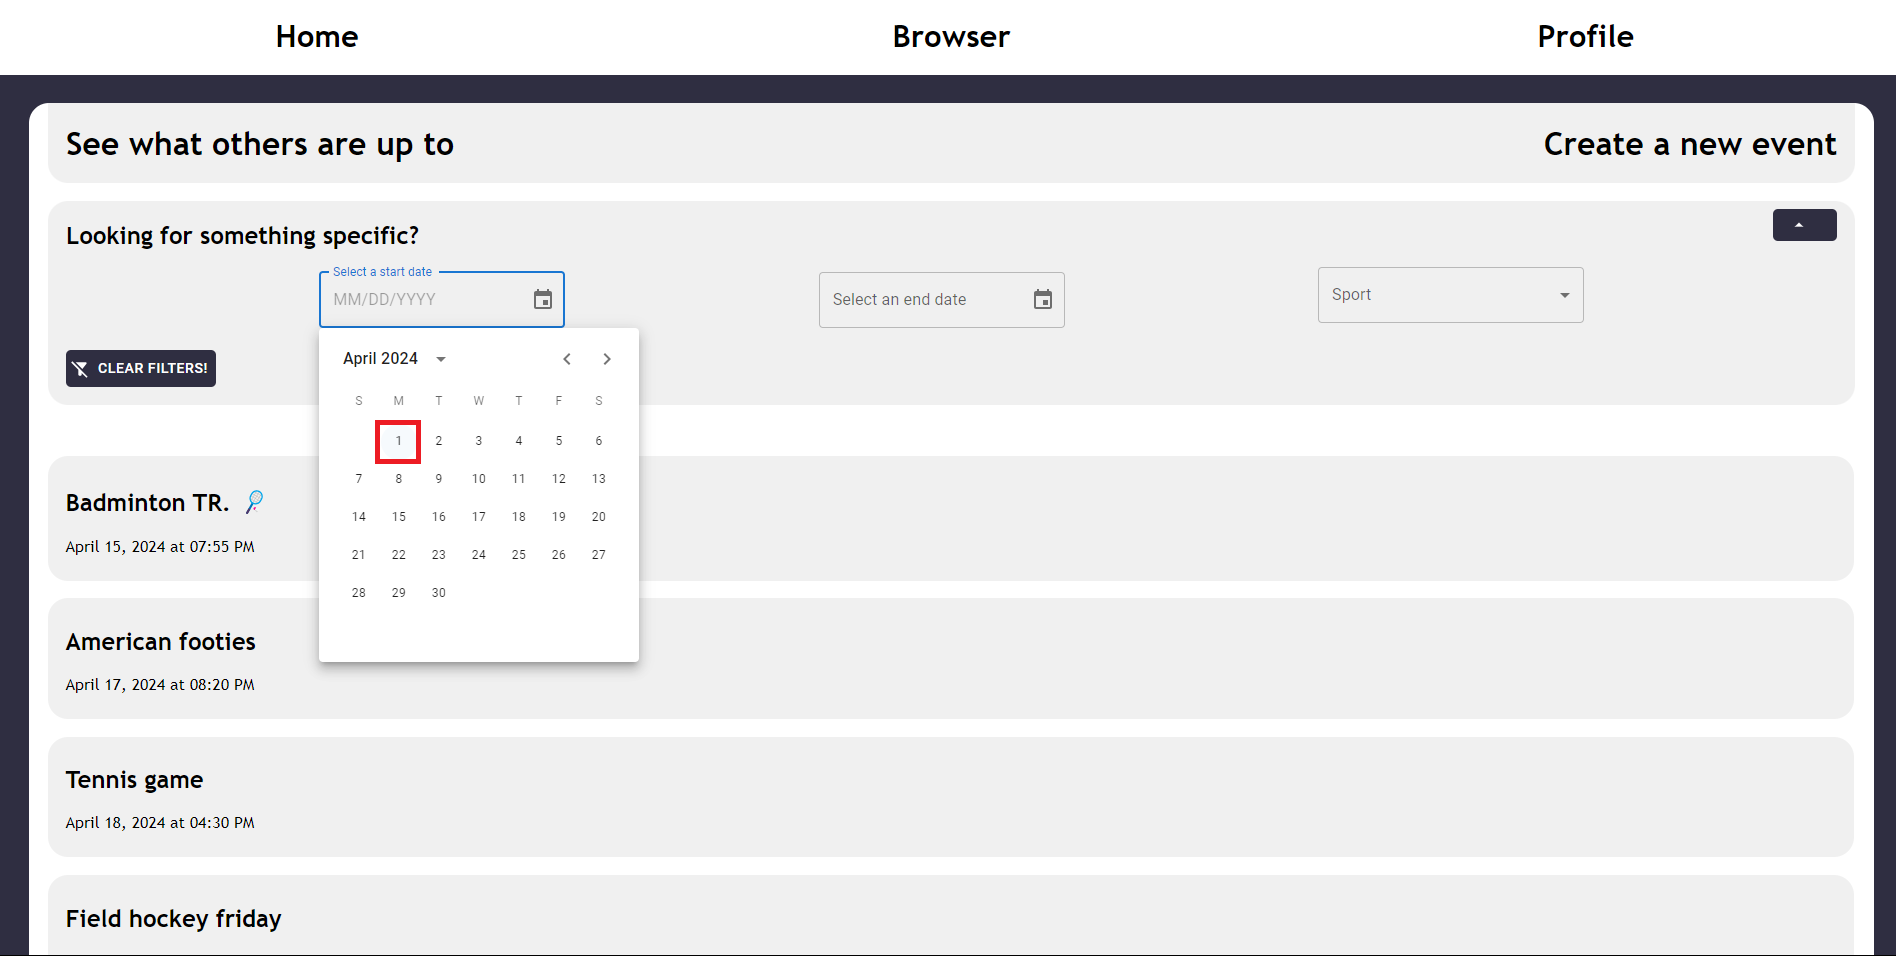
\includegraphics[width=0.5\textwidth]{images/filtering_events_2.png}
	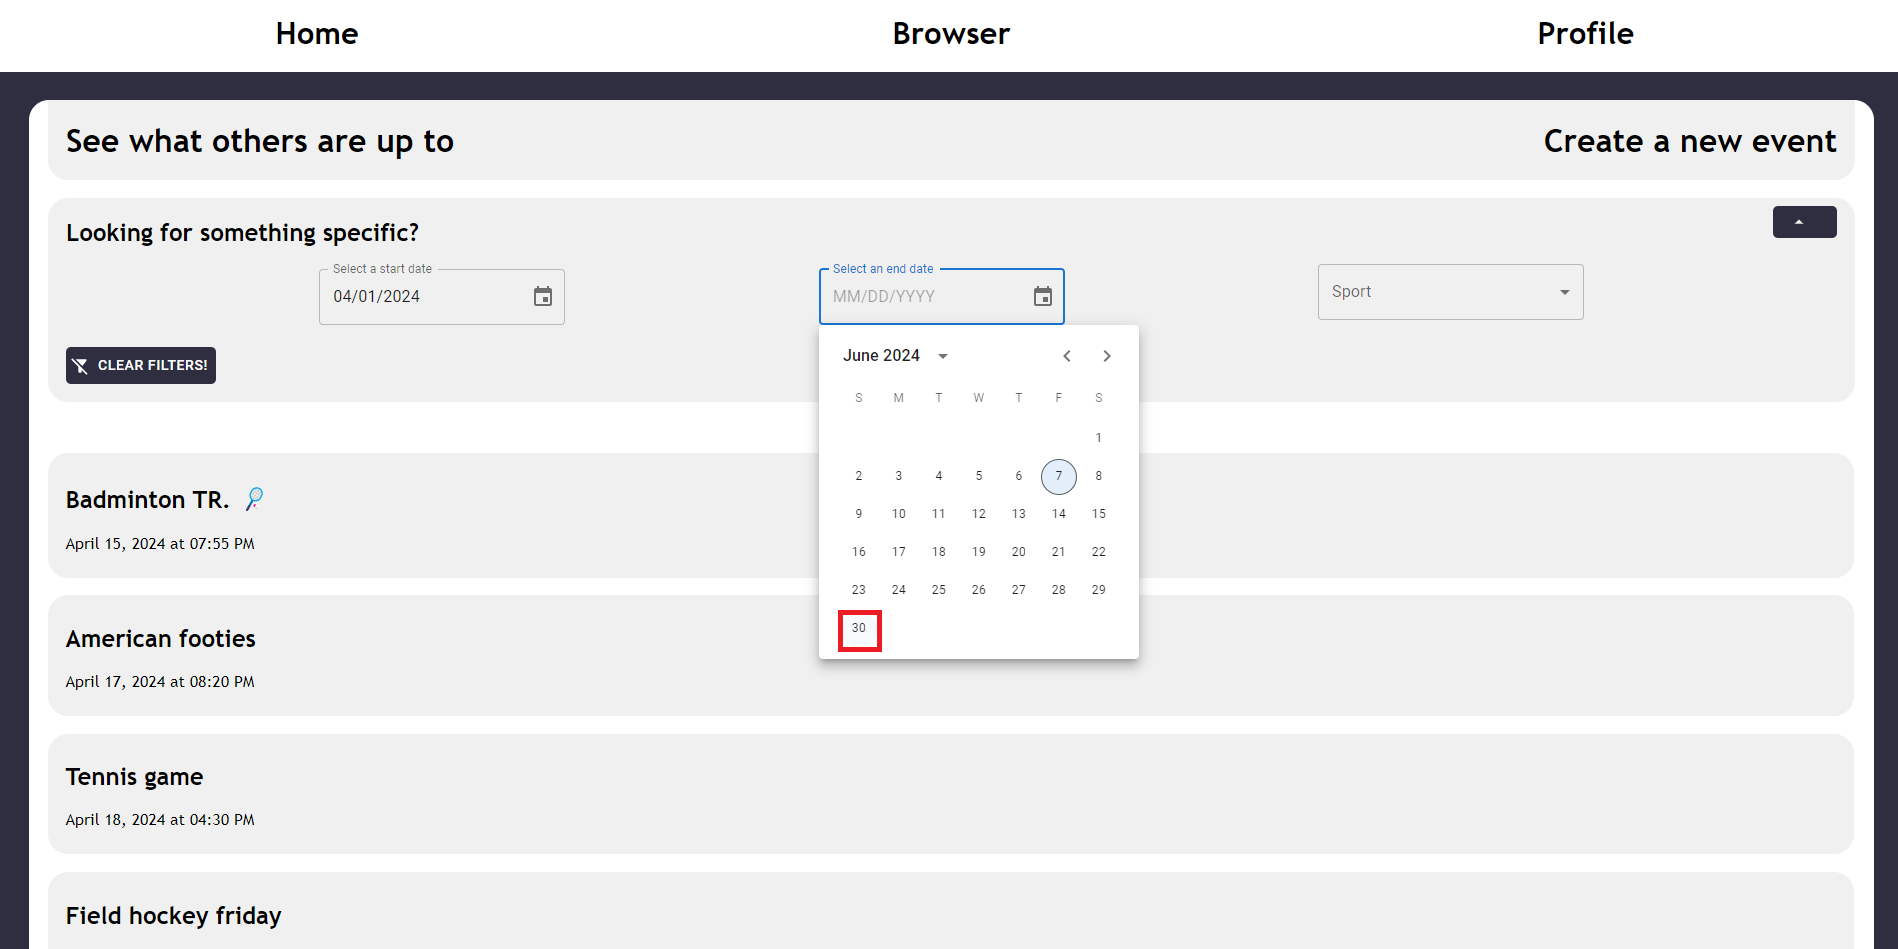
\includegraphics[width=0.5\textwidth]{images/filtering_events_3.png}
	\begin{center}
		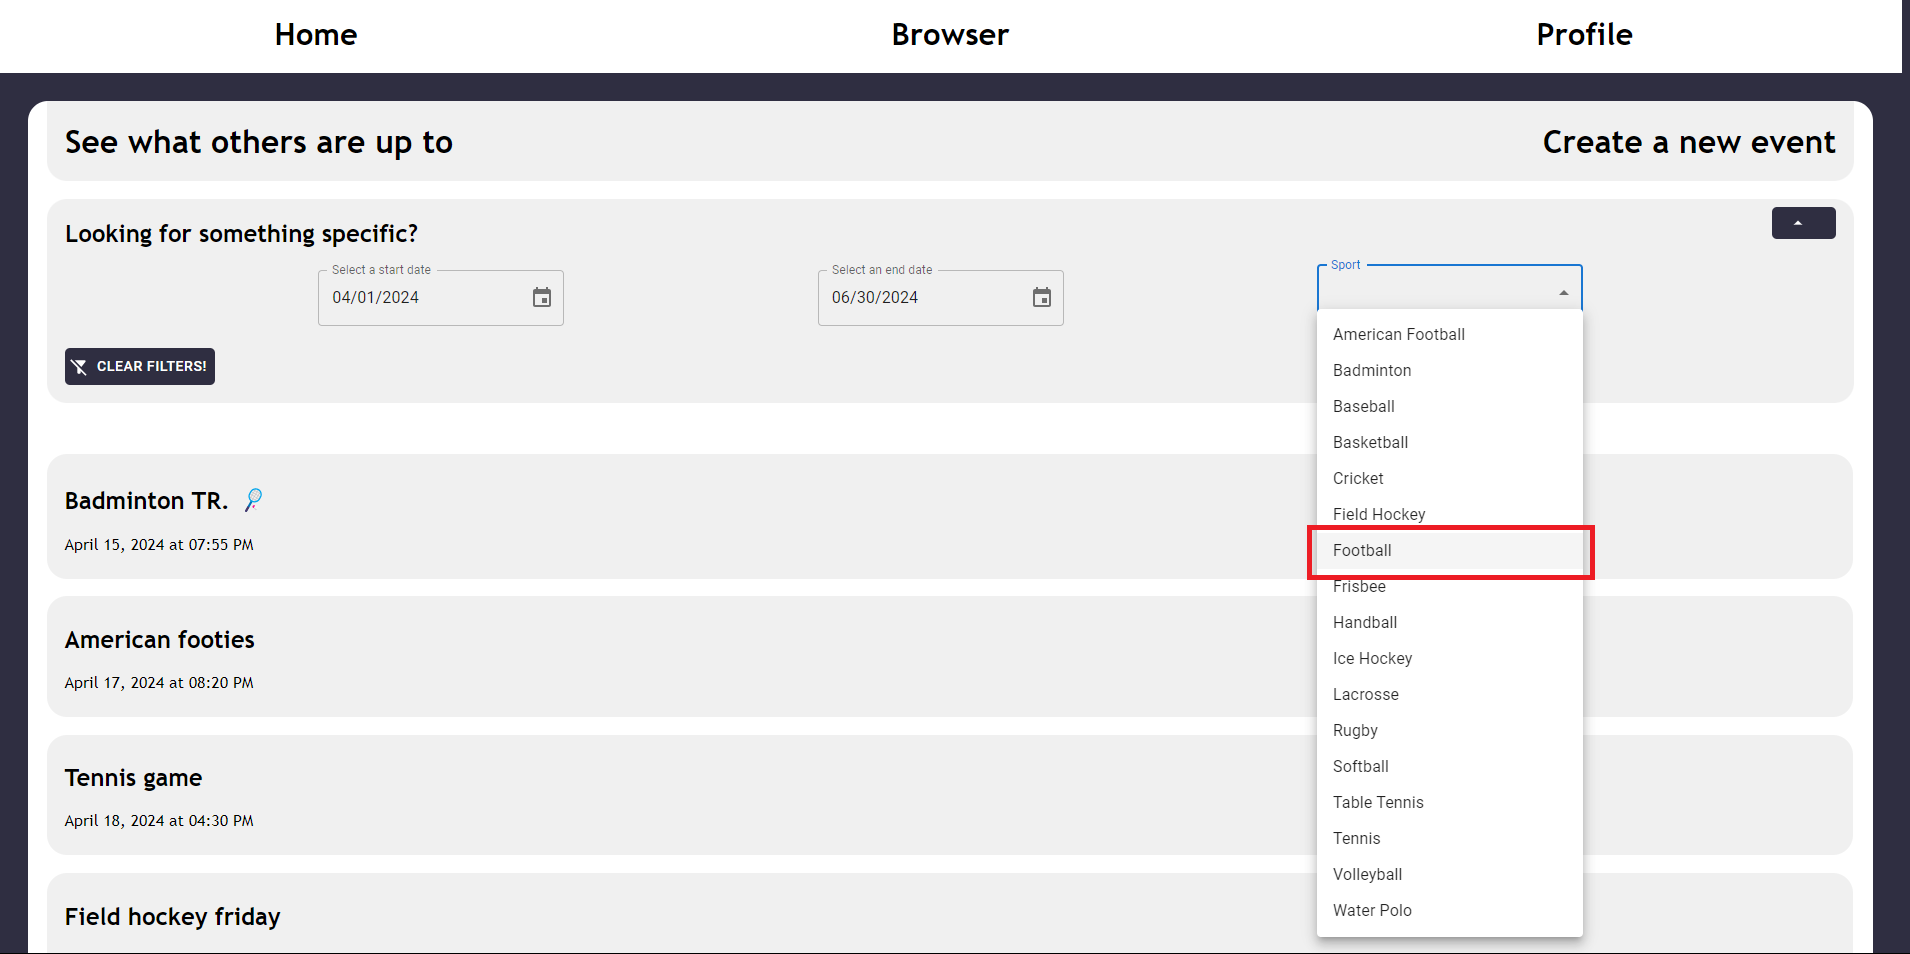
\includegraphics[width=0.5\textwidth]{images/filtering_events_4.png}
	\end{center}
	\caption{A szűrők beállítása}	
	\label{fig:applying_filters}
\end{figure}

Amint az látható a \ref{fig:applying_filters}-es ábrán, a szűrők beállítása után az oldal automatikusan frissül, és a beállított szűrőknek megfelelően
jeleníti meg az eseményeket. 

\begin{figure}
	\centering
	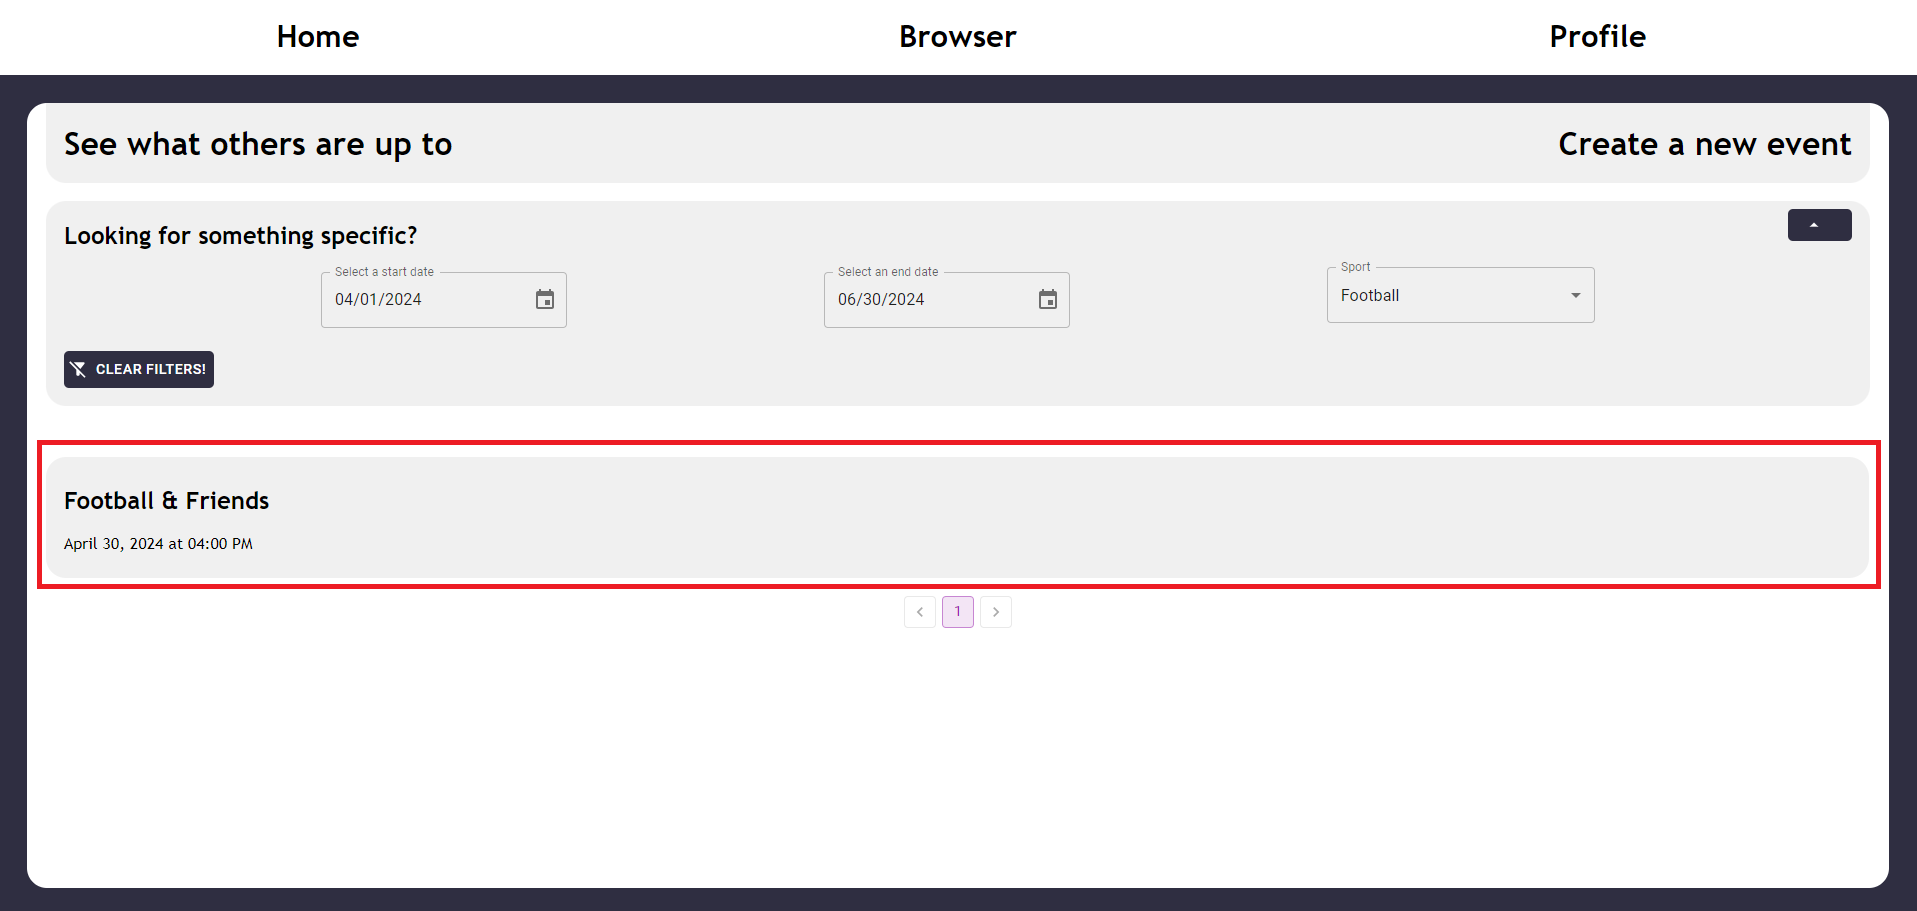
\includegraphics[width=0.7\textwidth]{images/filtering_events_5.png}
	\caption{A szűrt események}
	\label{fig:filtered_events}
\end{figure}

Ahogyan a \ref{fig:filtered_events}-es ábrán is látható, a szűrők alkalmazása egyetlen sporteseményt eredményezett.

\newpage
\section{Lapszámozás - Pagination}

Annak érdekében, hogy jó teljesítménnyel működhessen a webalkalmazás, szükséges az ú.n. \textit{Pagination}\cite{paginationdocs}, azaz az adatbázisból lekért sportesemények
szeletekre osztása. Ez azt jelenti, hogy nem fog mindeni felhasználó minden létező eseményt megkapni egy kérés során, hanem csak egy limitált számot,
melyek szekvenciális továbbá lekérhetőek.

Az alkalmazás automatikusan 5-ös szeletekre osztja a sporteseményeket, ezek között a lap alján van lehetősége a felhasználónak a navigáálásra. Ez látható a \ref{fig:pagination}-os ábrán.

\begin{figure}[ht]
	\centering
	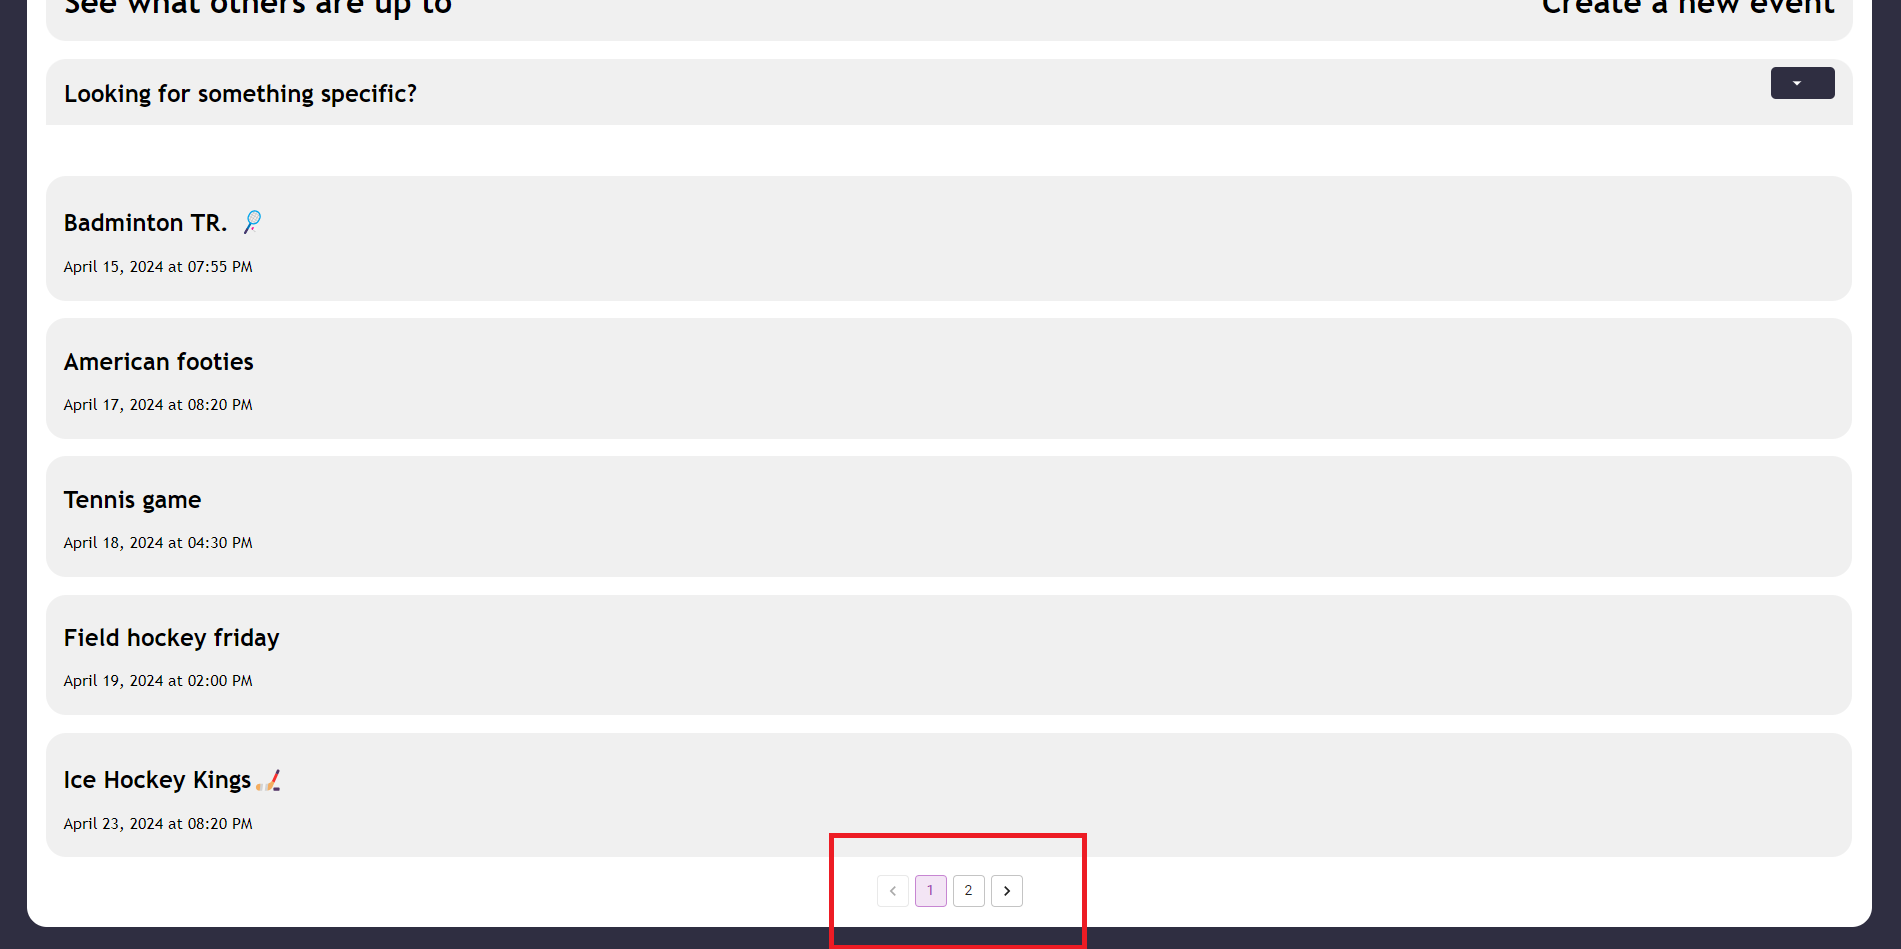
\includegraphics[width=0.7\textwidth]{images/pagination_1.png}
	\caption{A lapozás}
	\label{fig:pagination}
\end{figure}

Itt követehető az aktuális lap száma, illetve lehetőség van tovább haladásra a következő lapra, amennyiben ez létezik.
 %    %----------------------------------------------------------------------------
\chapter{Programok, technológiák bemutatása} \label{fejezet3}
%----------------------------------------------------------------------------

\section {Beépített szoftverek, könyvtárak}

Dolgozatom ezen részében előszőr vizsgáljunk meg olyan beépített differenciálegyenlet megoldó szoftvereket, melyeket már megemlítettem. Ezek közül én a Matlab és a Boost - Odeint beépített programját használtam és vizsgáltam meg. Mindkét esetben közönséges differenciálegyenletek (ODE) megoldására, az előre megírt algoritmus segítségével, melynek hátterében természetesen a Dormand-Prince módszer áll.


	\begin{align}
	x&=1+1+1+1\\
	&=4.
\end{align}

	\begin{align}
	y&=mx+b\nonumber\\
	z&=nw+c.
\end{align}

			\begin{align}
	\int_0^1\sum_a^b\prod_\alpha^\beta.
\end{align}
	\begin{align*}
	\frac{12}{34}.
\end{align*}
\subsection {Matlab - \href{https://www.mathworks.com/help/matlab/ref/ode45.html}{ode45}} \label{MatlabOde45}

A Matlab egy programcsomag és egyben egy technikai nyelv is, mely magas szinten lehetőséget biztosít számítások elvégzésére, modellezésre, szimulációra, megjelenítésre, vizualizációra és számos más hasznos mérnöki munka elvégzésére. Esetünkben a legfontosabb, hogy könnyedén tudunk közönséges differenciálegyenleteket megoldani az ode45 program segítségével. Emellett az eredményeket egy jól megtervezett felületen ki is tudjuk ábrázolni. Az alábbi példában jól látható, hogy milyen egyszerű és kényelmes a használata:

\begin{lstlisting}[caption={Matlab példakód diff. egyenlet megoldására.}, captionpos=b]
	f = @(t,y) y;
	t = [0 10];
	y0 = 1.0;
	ode45(f, t, y0);
	plot(t, y(:));
\end{lstlisting}


A fenti bemenetre $ n = 100 $ - szor lefuttattuk az algoritmust és a következő időeredményeket kaptuk:
\begin{itemize}
	\item Futási idők \textbf{átlaga}: $ 0.0043 $ sec
	\item Futási idők \textbf{minimuma}: $ 0.0026 $ sec
	\item Futási idők \textbf{maximuma}: $ 0.1504 $ sec
\end{itemize}




\begin{center}
\smartdiagram[flow diagram:horizontal]{Edit,
	\LaTeX, Bib\TeX/ biber, make\-index, \LaTeX}
\end{center}

\subsection {Boost - \href{http://headmyshoulder.github.io/odeint-v2/}{Odeint}} \label{BoostOdeint}

Egy másik előre megírt közönséges differenciálegyenlet megoldó a Boost könyvtárcsomag Odeint nevezetű könyvtára. Ez egy modern C++ nyelven írt csomag, lényeges jellemzői, hogy \textbf{nagy teljesítményre} képes és \textbf{nagyon magas szinten} (absztraktan - Template Metaprogramming) van megírva, így \textbf{rugalmas} és könnyen integrálható különböző rendszerekbe. Emellett rugalmas a bementi adatok típusát illetően is. Ugyanakkor jó tudni, hogy ez a nagyon absztrakt megvalósítás hátrány is lehet, mert bizonyos esetekben nagyon nehéz megérteni vagy megoldani egy felmerülő problémát. Most lássunk egy egyszerű példát a használatára:

\begin{lstlisting}[caption={Odeint példakód.}, captionpos=b, language = C++]
#include <iostream>
#include <boost/numeric/odeint.hpp>

using namespace std;
using namespace boost::numeric::odeint;

typedef runge_kutta_dopri5<double> stepper_type;

void rhs( const double x , double &dxdt , const double t ) {
	dxdt = 3.0/(2.0*t*t) + x/(2.0*t);
}

void write_cout( const double &x , const double t ) {
	cout << t << '\t' << x << endl;
}

int main() {
	double x = 0.0;    
	integrate_adaptive( make_controlled( 1E-12 , 1E-12 , stepper_type() ) ,
	rhs , x , 1.0 , 10.0 , 0.1 , write_cout );
}
\end{lstlisting}
\pagebreak
Az előző kódrészlet eredménye a következő:



\begin{itemize}
	\item Futási idők \textbf{átlaga}: $ 0.0989 $ sec
	\item Futási idők \textbf{minimuma}: $ 0.09 $ sec
	\item Futási idők \textbf{maximuma}: $ 0.099 $ sec
\end{itemize}

\section {Általam megvalósított szoftverek} \label{fejezet3_2}

\begin{lstlisting}[caption={Matlab kód ode45 használata nélkül.}, captionpos=b, language = Matlab]
function [yy, tt, timeSpent] = fun_dopri45(f, y0, t0, tf, tolerance)
	...
	while t < tf
		if (t+h >= tf)
			h = tf-t;
		end
		
		% Calculate k1, k2, ... , k7
		k1 = h*feval(f, t+h*C(1), y);
		k2 = h*feval(f, t+h*C(2), y + A2(1)*k1);
		...
		k7 = h*feval(f, t+h*C(7), y + A7(1)*k1 + A7(3)*k3 + ... + A7(6)*k6);
		
		% Calcaulate the next point
		yt = y + A7(1)*k1 + A7(3)*k3 + A7(4)*k4 + A7(5)*k5 + A7(6)*k6;
		% Calculate the error
		err = abs(E(1)*k1 + E(3)*k3 + ... + E(7)*k7);
		
		if max(err) < tolerance
			t = t + h;
			y = yt;
			...
		end
		
		% Calculate optimal step size
		scale = 1.25*(maxErr/tolerance)^(1/5);
		if scale > 0.2
			h = h / scale;
		else
			h = 5.0*h;
		end
	end
end
\end{lstlisting}

\begin{itemize}
	\item Futási idők \textbf{átlaga}: $ 0.0043 $ sec
	\item Futási idők \textbf{minimuma}: $ 0.0058 $ sec
	\item Futási idők \textbf{maximuma}: $ 0.0287 $ sec
\end{itemize}

A következő szoftvert, amit bemutatok \textbf{Java} nyelven írtam objektum orientáltan, a fejlesztés során pedig Eclipse fejlesztői környezetet használtam. Ez a szoftver három egységből áll: fő -, differenciálegyenlet megoldó - és kifejezés kiértékelő egység (ezt a legnehezebb megvalósítani vagy megtalálni a megfelelő könyvtárat). Az alkalmazás nem rendelkezik grafikus felhasználói felülettel, a bemeneti adatokat egy szöveges állományból olvassa be (amelynek jól meghatározott szerkezete van) és a kívánt eredményeket a standard kimenetre írja ki. A kifejezés kiértékelő egység megírásánál felhasználtam egy előre elkészített Java könyvtárat, melyet \href{http://www.singularsys.com/jep/}{\textit{JEP}}-nek neveznek. A szoftverben arra használtam fel, hogy egy sztringként megadott kifejezést kiértékeltem és elvégeztem a segítségével. Mindezt úgy csinálja, hogy a háttérben felépít egy kifejezésfát, aminek a leveleiben lesznek az értékek, csúcsaiban a műveletek, zárójelek, stb. (lásd az alábbi ábrát):



\begin{itemize}
	\item Futási idők \textbf{átlaga}: $ 0.1422 $ sec
	\item Futási idők \textbf{minimuma}: $ 0.123 $ sec
	\item Futási idők \textbf{maximuma}: $ 0.341 $ sec
\end{itemize}

Harmadiként lássuk a \textbf{C++ szoftvert}, amelyet szintén objektum orientáltam valósítottam meg. Ennek a szoftvernek a szerkezete hasonló a Java szoftver szerkezetéhez. Ebben az esetben is szükség volt egy kifejezés kiértékelő könyvtárra, hogy ne kelljen egy sajátot írni. Először kipróbáltam egy \href{http://beltoforion.de/article.php?a=muparser}{\textit{muparser}} nevű könytárat, aztán egy másikat is, aminek \href{https://exprtk.codeplex.com/}{\textit{ExprTk}} (Expression Toolkit Library) a neve. Fontos elmondani, hogy mindkét könyvtár ingyenesen elérhető és használható. Az első könyvtárat nehezebb volt hozzáadni a szoftverhez és mivel több fájlból állt több időbe került a fordítása is. A legfőbb ok, amiért mégis a másodikat használtam az volt, hogy jelentősen gyorsabb és hatékonyabb volt az én szoftveremben. Tehát végül az \textit{ExprTk} könyvtárat használtam a jobb teljesítménye és könnyebb integrálhatósága miatt.


\begin{itemize}
	\item Futási idők \textbf{átlaga}: $ 0.1086 $ sec
	\item Futási idők \textbf{minimuma}: $ 0.096 $ sec
	\item Futási idők \textbf{maximuma}: $ 0.214 $ sec
\end{itemize}

Végül nézzük meg az utolsó, Dormand-Prince módszeren alapuló szoftvert, amely egy \textbf{Android alkalmazás}. Mint tudjuk napjainkban a mobileszközök nagyon elterjedtek és teljesítményük is jelentősen megnőtt, lassan felveszik a versenyt a személyi számítógépekkel. Ezért mindenképp szerettem volna az algoritmust megvalósítani mobileszközökre is és megnézni itt is a teljesítményt. Mivel az Android alkalmazások fejlesztésénél Java nyelvet használunk, így könnyű dolgom volt, hiszen a Java szoftverből át tudtam venni a már jól megírt és elkülönített osztályokat. Ugyanazt a \textit{JEP} könyvtárat használtam itt is a kifejezések kiértékelésére, így majd az eredmények összehasonlítását is könnyebbé tettem. A Java és C++ szoftverrel ellentétben rendelkezik egy kis grafikus felhasználói felülettel, de a bemeneti adatokat itt is egy szöveges állományból olvassuk be, mert nem túl kényelmes azt a sok számadatot, meg egyenletet beviteli mezőkön keresztűl beírni.


\begin{itemize}
	\item Futási idők \textbf{átlaga}: $ 37.9015 $ sec
	\item Futási idők \textbf{minimuma}: $ 31.116 $ sec
	\item Futási idők \textbf{maximuma}: $ 70.876 $ sec
\end{itemize}

\section {Szoftverek összehasonlítása} \label{fejezet3_3}

Az előző alfejezetekben ismertettem a már létező Dormand-Prince módszeren alapú differenciálegyenlet megoldók közül kettőt és négy saját megvalósítást is. Mindegyik esetében láthattunk futási időket és számadatokat, azonban nem láttuk ezeket egymás mellett. Ebben az alfejezetben összegezzük és összehasonlítjuk a kapott eredményeket.

Fontos, hogy minden algoritmust ugyanazon a hardveren teszteljünk, mert csak így reálisak és összehasonlíthatóak a mérési adatok. Esetünkben használt hardver konfigurációja:
\begin{itemize}
	\item Intel Core i5-7200U, 2.50 GHz processzor, 8.00 GB RAM memória
\end{itemize}
Természetesen az Android alkamazást csak mobileszközökön lehetett vizsgálni, itt két készüléket használtam a tesztelésre:
\begin{itemize}
	\item Motorola Moto E2, Quad-core 1.2 GHz processzor, 1 GB RAM memória
	\item Samsung Galaxy Core Prime, Quad-core 1.2 GHz processzor, 1 GB RAM memória
\end{itemize}


\begin{table}[h!]
	\centering
	\begin{tabular}{ | l | c | c | c | c |}
		\hline 
		\textbf{Technológia} & \textbf{Átlagidő (s)} & \textbf{Min. idő (s)} & \textbf{Max. idő (s)} & \textbf{Hardver}\\
		\hline
		Matlab - ode45 & $ 0.0032 $ & $ 0.0029 $ & $ 0.0038 $ & Intel Core i5\\
		\hline
		Boost - Odeint & $ 0.0989 $ & $ 0.0900 $ & $ 0.1290 $ & Intel Core i5\\
		\hline
		Matlab & $ 0.0062 $ & $ 0.0060 $ & $ 0.0066 $ & Intel Core i5\\
		\hline
		Java & $ 0.2224 $ & $ 0.1970 $ & $ 0.3020 $ & Intel Core i5\\ 
		\hline
		C++ & $ 0.1047 $ & $ 0.1010 $ & $ 0.1240 $ & Intel Core i5\\
		\hline
		Android & $ 37.9015 $ & $ 31.1160 $ & $ 70.8760 $ & Moto E2\\
		\hline
		Android & $ 35.9987 $ & $ 29.4200 $ & $ 87.6120 $ & Core Prime\\
		\hline
	\end{tabular}
	\caption{Mérési eredmények  $ n = 10 $ tesztesetre.}
	\label{tablazat1}
\end{table}

\begin{table}[h!]
	\centering
	\begin{tabular}{ | l | c | c | c | c |}
		\hline 
		\textbf{Technológia} & \textbf{Átlagidő (s)} & \textbf{Min. idő (s)} & \textbf{Max. idő (s)} & \textbf{Hardver}\\
		\hline
		Matlab - ode45 & $ 0.0043 $ & $ 0.0026 $ & $ 0.1504 $ & Intel Core i5\\
		\hline
		Boost - Odeint & $ 0.0912 $ & $ 0.0900 $ & $ 0.0990 $ & Intel Core i5\\
		\hline
		Matlab & $ 0.0067 $ & $ 0.0058 $ & $ 0.0287 $ & Intel Core i5\\
		\hline
		Java & $ 0.1422 $ & $ 0.1230 $ & $ 0.3410 $ & Intel Core i5\\ 
		\hline
		C++ & $ 0.1086 $ & $ 0.0960 $ & $ 0.2140 $ & Intel Core i5\\
		\hline
		Android & $ - $ & $ - $ & $ - $ & Moto E2\\
		\hline
		Android & $ - $ & $ - $ & $ - $ & Core Prime\\
		\hline
	\end{tabular}
	\caption{Mérési eredmények  $ n = 100 $ tesztesetre.}
\end{table}



\section {Differenciálegyenletek megoldása GPU-n} \label{fejezet3_4}


A továbbiakban nézzük meg a két algoritmus magjának szekvenciális és párhuzamosított változatait:
\begin{lstlisting}[caption={Euler módszer szekvenciális kód.}, captionpos=b, language = C++]
for (int i = 0; i < numberOfVariables; ++i) {
	mResult.at(i)[j + 1] = mResult.at(i)[j] + mInputs->getStepSize() *
	(mFunctionsParsers.at(i)->computeFunctionValue(values));
}
\end{lstlisting}

\begin{lstlisting}[caption={Euler módszer párhuzamosított kód.}, captionpos=b, language = C++]
__global__ void computeFunctionsValuesKernel(double* resultValues,
double* previousValues, double* functionValues, double stepSize, int N) {
	int i = threadIdx.x;
	
	if (i < N) {
		resultValues[i] = previousValues[i] + stepSize * functionValues[i];
	}
}
\end{lstlisting}

\begin{lstlisting}[caption={Runge-Kutta módszer szekvenciális kód.}, captionpos=b, language = C++]
for (int k = 0; k < numberOfVariables; ++k) {
	mResult.at(k)[i + 1] = mResult.at(k)[i] + (mInputs->getStepSize() / 6)*
	(K[0][k] + 2 * K[1][k] + 2 * K[2][k] + K[3][k]);
}
\end{lstlisting}

\begin{lstlisting}[caption={Runge-Kutta módszer párhuzamosított kód.}, captionpos=b, language = C++]
__global__ void computeValuesKernel(double* resultValues, double* K,
double* previousValues, double stepSize, int numberOfVariables) {
	int i = threadIdx.x;
	
	if (i < numberOfVariables) {
		resultValues[i] = previousValues[i] + ((stepSize / 6) *
		(K[i] + 2 * K[i + 1 * numberOfVariables] +
		2 * K[i + 2 * numberOfVariables] + K[i + 3 * numberOfVariables]));
	}
}
\end{lstlisting}

Nézzünk meg pár mérési eredményt a következő differenciálegyenlet rendszerre:
\begin{align}
	\begin{cases}
		y_{1}'(t, y) = y_{1} \\
		\vdots \\
		y_{n}'(t, y) = y_{n}\\
		y_{1}'(t_{0}) = 1.0 \\
		\vdots \\
		y_{n}'(t_{0}) = 1.0\\
	\end{cases}
	, t\in[0, 100], n = 5
\end{align}

\begin{table}[h!]
	\centering
	\begin{tabular}{ | p{1.8cm} | p{2.5cm} | p{2.5cm} | p{2.5cm} | p{2.5cm} |}
		\hline  & \multicolumn{2}{|c|}{\textbf{CPU sec (Intel Core i5)}} & \multicolumn{2}{|c|}{\textbf{GPU sec (GeForce 940MX)}}\\ 
		\hline  & Euler & Runge-Kutta & Euler & Runge-Kutta\\ 
		\hline
		$ h = 10.0 $ & $ 0.006 $ & $ 0.036 $ & $ 0.587 $ & $ 0.036 $ \\ 
		\hline
		$ h = 1.0 $ & $ 0.074 $ & $ 0.523 $ & $ 0.841 $ & $ 0.490 $ \\
		\hline
		$ h = 0.1 $ & $ 0.689 $ & $ 4.987 $ & $ 1.565 $ & $ 3.399 $ \\
		\hline
		$ h = 0.01 $ & $ 7.202 $ & $ 52.800 $ & $ 14.321 $ & $ 50.110 $ \\
		\hline
		$ h = 0.001 $ & $ 71.071 $ & $ 500.999 $ & $ 98.445 $ & $ 321.965 $ \\
		\hline
	\end{tabular}
	\caption{Mérési eredmények $ n = 5 $ egyenlet esetén.}
\end{table}

\begin{align}
	\begin{cases}
		y_{1}'(t, y) = y_{1} \\
		\vdots \\
		y_{n}'(t, y) = y_{n}\\
		y_{1}'(t_{0}) = 1.0 \\
		\vdots \\
		y_{n}'(t_{0}) = 1.0\\
	\end{cases}
	, t\in[0, 100], n = 10
\end{align}

\begin{table}[h!]
	\centering
	\begin{tabular}{ | p{1.8cm} | p{2.5cm} | p{2.5cm} | p{2.5cm} | p{2.5cm} |}
		\hline  & \multicolumn{2}{|c|}{\textbf{CPU sec (Intel Core i7)}} & \multicolumn{2}{|c|}{\textbf{GPU sec (GeForce 950M)}}\\ 
		\hline  & Euler & Runge-Kutta & Euler & Runge-Kutta\\ 
		\hline
		$ h = 10.0 $ & $ 0.039 $ & $ 0.256 $ & $ 1.070 $ & $ 0.222 $ \\ 
		\hline
		$ h = 1.0 $ & $ 0.320 $ & $ 2.482 $ & $ 0.994 $ & $ 2.087 $ \\
		\hline
		$ h = 0.1 $ & $ 3.042 $ & $ 23.962 $ & $ 4.143 $ & $ 20.978 $ \\
		\hline
		$ h = 0.01 $ & $ 30.812 $ & $ 241.977 $ & $ 35.009 $ & $ 206.842 $ \\
		\hline
		$ h = 0.001 $ & $ 305.092 $ & $ 2394.930 $ & $ 344.485 $ & $ 2067.870 $ \\
		\hline
	\end{tabular}
	\caption{Mérési eredmények $ n = 10 $ egyenlet esetén.}
\end{table}


	% %----------------------------------------------------------------------------
\chapter{Programok, technológiák bemutatása} \label{fejezet3}
%----------------------------------------------------------------------------

\section {Beépített szoftverek, könyvtárak}

Dolgozatom ezen részében előszőr vizsgáljunk meg olyan beépített differenciálegyenlet megoldó szoftvereket, melyeket már megemlítettem. Ezek közül én a Matlab és a Boost - Odeint beépített programját használtam és vizsgáltam meg. Mindkét esetben közönséges differenciálegyenletek (ODE) megoldására, az előre megírt algoritmus segítségével, melynek hátterében természetesen a Dormand-Prince módszer áll.


	\begin{align}
	x&=1+1+1+1\\
	&=4.
\end{align}

	\begin{align}
	y&=mx+b\nonumber\\
	z&=nw+c.
\end{align}

			\begin{align}
	\int_0^1\sum_a^b\prod_\alpha^\beta.
\end{align}
	\begin{align*}
	\frac{12}{34}.
\end{align*}
\subsection {Matlab - \href{https://www.mathworks.com/help/matlab/ref/ode45.html}{ode45}} \label{MatlabOde45}

A Matlab egy programcsomag és egyben egy technikai nyelv is, mely magas szinten lehetőséget biztosít számítások elvégzésére, modellezésre, szimulációra, megjelenítésre, vizualizációra és számos más hasznos mérnöki munka elvégzésére. Esetünkben a legfontosabb, hogy könnyedén tudunk közönséges differenciálegyenleteket megoldani az ode45 program segítségével. Emellett az eredményeket egy jól megtervezett felületen ki is tudjuk ábrázolni. Az alábbi példában jól látható, hogy milyen egyszerű és kényelmes a használata:

\begin{lstlisting}[caption={Matlab példakód diff. egyenlet megoldására.}, captionpos=b]
	f = @(t,y) y;
	t = [0 10];
	y0 = 1.0;
	ode45(f, t, y0);
	plot(t, y(:));
\end{lstlisting}


A fenti bemenetre $ n = 100 $ - szor lefuttattuk az algoritmust és a következő időeredményeket kaptuk:
\begin{itemize}
	\item Futási idők \textbf{átlaga}: $ 0.0043 $ sec
	\item Futási idők \textbf{minimuma}: $ 0.0026 $ sec
	\item Futási idők \textbf{maximuma}: $ 0.1504 $ sec
\end{itemize}




\begin{center}
\smartdiagram[flow diagram:horizontal]{Edit,
	\LaTeX, Bib\TeX/ biber, make\-index, \LaTeX}
\end{center}

\subsection {Boost - \href{http://headmyshoulder.github.io/odeint-v2/}{Odeint}} \label{BoostOdeint}

Egy másik előre megírt közönséges differenciálegyenlet megoldó a Boost könyvtárcsomag Odeint nevezetű könyvtára. Ez egy modern C++ nyelven írt csomag, lényeges jellemzői, hogy \textbf{nagy teljesítményre} képes és \textbf{nagyon magas szinten} (absztraktan - Template Metaprogramming) van megírva, így \textbf{rugalmas} és könnyen integrálható különböző rendszerekbe. Emellett rugalmas a bementi adatok típusát illetően is. Ugyanakkor jó tudni, hogy ez a nagyon absztrakt megvalósítás hátrány is lehet, mert bizonyos esetekben nagyon nehéz megérteni vagy megoldani egy felmerülő problémát. Most lássunk egy egyszerű példát a használatára:

\begin{lstlisting}[caption={Odeint példakód.}, captionpos=b, language = C++]
#include <iostream>
#include <boost/numeric/odeint.hpp>

using namespace std;
using namespace boost::numeric::odeint;

typedef runge_kutta_dopri5<double> stepper_type;

void rhs( const double x , double &dxdt , const double t ) {
	dxdt = 3.0/(2.0*t*t) + x/(2.0*t);
}

void write_cout( const double &x , const double t ) {
	cout << t << '\t' << x << endl;
}

int main() {
	double x = 0.0;    
	integrate_adaptive( make_controlled( 1E-12 , 1E-12 , stepper_type() ) ,
	rhs , x , 1.0 , 10.0 , 0.1 , write_cout );
}
\end{lstlisting}
\pagebreak
Az előző kódrészlet eredménye a következő:



\begin{itemize}
	\item Futási idők \textbf{átlaga}: $ 0.0989 $ sec
	\item Futási idők \textbf{minimuma}: $ 0.09 $ sec
	\item Futási idők \textbf{maximuma}: $ 0.099 $ sec
\end{itemize}

\section {Általam megvalósított szoftverek} \label{fejezet3_2}

\begin{lstlisting}[caption={Matlab kód ode45 használata nélkül.}, captionpos=b, language = Matlab]
function [yy, tt, timeSpent] = fun_dopri45(f, y0, t0, tf, tolerance)
	...
	while t < tf
		if (t+h >= tf)
			h = tf-t;
		end
		
		% Calculate k1, k2, ... , k7
		k1 = h*feval(f, t+h*C(1), y);
		k2 = h*feval(f, t+h*C(2), y + A2(1)*k1);
		...
		k7 = h*feval(f, t+h*C(7), y + A7(1)*k1 + A7(3)*k3 + ... + A7(6)*k6);
		
		% Calcaulate the next point
		yt = y + A7(1)*k1 + A7(3)*k3 + A7(4)*k4 + A7(5)*k5 + A7(6)*k6;
		% Calculate the error
		err = abs(E(1)*k1 + E(3)*k3 + ... + E(7)*k7);
		
		if max(err) < tolerance
			t = t + h;
			y = yt;
			...
		end
		
		% Calculate optimal step size
		scale = 1.25*(maxErr/tolerance)^(1/5);
		if scale > 0.2
			h = h / scale;
		else
			h = 5.0*h;
		end
	end
end
\end{lstlisting}

\begin{itemize}
	\item Futási idők \textbf{átlaga}: $ 0.0043 $ sec
	\item Futási idők \textbf{minimuma}: $ 0.0058 $ sec
	\item Futási idők \textbf{maximuma}: $ 0.0287 $ sec
\end{itemize}

A következő szoftvert, amit bemutatok \textbf{Java} nyelven írtam objektum orientáltan, a fejlesztés során pedig Eclipse fejlesztői környezetet használtam. Ez a szoftver három egységből áll: fő -, differenciálegyenlet megoldó - és kifejezés kiértékelő egység (ezt a legnehezebb megvalósítani vagy megtalálni a megfelelő könyvtárat). Az alkalmazás nem rendelkezik grafikus felhasználói felülettel, a bemeneti adatokat egy szöveges állományból olvassa be (amelynek jól meghatározott szerkezete van) és a kívánt eredményeket a standard kimenetre írja ki. A kifejezés kiértékelő egység megírásánál felhasználtam egy előre elkészített Java könyvtárat, melyet \href{http://www.singularsys.com/jep/}{\textit{JEP}}-nek neveznek. A szoftverben arra használtam fel, hogy egy sztringként megadott kifejezést kiértékeltem és elvégeztem a segítségével. Mindezt úgy csinálja, hogy a háttérben felépít egy kifejezésfát, aminek a leveleiben lesznek az értékek, csúcsaiban a műveletek, zárójelek, stb. (lásd az alábbi ábrát):



\begin{itemize}
	\item Futási idők \textbf{átlaga}: $ 0.1422 $ sec
	\item Futási idők \textbf{minimuma}: $ 0.123 $ sec
	\item Futási idők \textbf{maximuma}: $ 0.341 $ sec
\end{itemize}

Harmadiként lássuk a \textbf{C++ szoftvert}, amelyet szintén objektum orientáltam valósítottam meg. Ennek a szoftvernek a szerkezete hasonló a Java szoftver szerkezetéhez. Ebben az esetben is szükség volt egy kifejezés kiértékelő könyvtárra, hogy ne kelljen egy sajátot írni. Először kipróbáltam egy \href{http://beltoforion.de/article.php?a=muparser}{\textit{muparser}} nevű könytárat, aztán egy másikat is, aminek \href{https://exprtk.codeplex.com/}{\textit{ExprTk}} (Expression Toolkit Library) a neve. Fontos elmondani, hogy mindkét könyvtár ingyenesen elérhető és használható. Az első könyvtárat nehezebb volt hozzáadni a szoftverhez és mivel több fájlból állt több időbe került a fordítása is. A legfőbb ok, amiért mégis a másodikat használtam az volt, hogy jelentősen gyorsabb és hatékonyabb volt az én szoftveremben. Tehát végül az \textit{ExprTk} könyvtárat használtam a jobb teljesítménye és könnyebb integrálhatósága miatt.


\begin{itemize}
	\item Futási idők \textbf{átlaga}: $ 0.1086 $ sec
	\item Futási idők \textbf{minimuma}: $ 0.096 $ sec
	\item Futási idők \textbf{maximuma}: $ 0.214 $ sec
\end{itemize}

Végül nézzük meg az utolsó, Dormand-Prince módszeren alapuló szoftvert, amely egy \textbf{Android alkalmazás}. Mint tudjuk napjainkban a mobileszközök nagyon elterjedtek és teljesítményük is jelentősen megnőtt, lassan felveszik a versenyt a személyi számítógépekkel. Ezért mindenképp szerettem volna az algoritmust megvalósítani mobileszközökre is és megnézni itt is a teljesítményt. Mivel az Android alkalmazások fejlesztésénél Java nyelvet használunk, így könnyű dolgom volt, hiszen a Java szoftverből át tudtam venni a már jól megírt és elkülönített osztályokat. Ugyanazt a \textit{JEP} könyvtárat használtam itt is a kifejezések kiértékelésére, így majd az eredmények összehasonlítását is könnyebbé tettem. A Java és C++ szoftverrel ellentétben rendelkezik egy kis grafikus felhasználói felülettel, de a bemeneti adatokat itt is egy szöveges állományból olvassuk be, mert nem túl kényelmes azt a sok számadatot, meg egyenletet beviteli mezőkön keresztűl beírni.


\begin{itemize}
	\item Futási idők \textbf{átlaga}: $ 37.9015 $ sec
	\item Futási idők \textbf{minimuma}: $ 31.116 $ sec
	\item Futási idők \textbf{maximuma}: $ 70.876 $ sec
\end{itemize}

\section {Szoftverek összehasonlítása} \label{fejezet3_3}

Az előző alfejezetekben ismertettem a már létező Dormand-Prince módszeren alapú differenciálegyenlet megoldók közül kettőt és négy saját megvalósítást is. Mindegyik esetében láthattunk futási időket és számadatokat, azonban nem láttuk ezeket egymás mellett. Ebben az alfejezetben összegezzük és összehasonlítjuk a kapott eredményeket.

Fontos, hogy minden algoritmust ugyanazon a hardveren teszteljünk, mert csak így reálisak és összehasonlíthatóak a mérési adatok. Esetünkben használt hardver konfigurációja:
\begin{itemize}
	\item Intel Core i5-7200U, 2.50 GHz processzor, 8.00 GB RAM memória
\end{itemize}
Természetesen az Android alkamazást csak mobileszközökön lehetett vizsgálni, itt két készüléket használtam a tesztelésre:
\begin{itemize}
	\item Motorola Moto E2, Quad-core 1.2 GHz processzor, 1 GB RAM memória
	\item Samsung Galaxy Core Prime, Quad-core 1.2 GHz processzor, 1 GB RAM memória
\end{itemize}


\begin{table}[h!]
	\centering
	\begin{tabular}{ | l | c | c | c | c |}
		\hline 
		\textbf{Technológia} & \textbf{Átlagidő (s)} & \textbf{Min. idő (s)} & \textbf{Max. idő (s)} & \textbf{Hardver}\\
		\hline
		Matlab - ode45 & $ 0.0032 $ & $ 0.0029 $ & $ 0.0038 $ & Intel Core i5\\
		\hline
		Boost - Odeint & $ 0.0989 $ & $ 0.0900 $ & $ 0.1290 $ & Intel Core i5\\
		\hline
		Matlab & $ 0.0062 $ & $ 0.0060 $ & $ 0.0066 $ & Intel Core i5\\
		\hline
		Java & $ 0.2224 $ & $ 0.1970 $ & $ 0.3020 $ & Intel Core i5\\ 
		\hline
		C++ & $ 0.1047 $ & $ 0.1010 $ & $ 0.1240 $ & Intel Core i5\\
		\hline
		Android & $ 37.9015 $ & $ 31.1160 $ & $ 70.8760 $ & Moto E2\\
		\hline
		Android & $ 35.9987 $ & $ 29.4200 $ & $ 87.6120 $ & Core Prime\\
		\hline
	\end{tabular}
	\caption{Mérési eredmények  $ n = 10 $ tesztesetre.}
	\label{tablazat1}
\end{table}

\begin{table}[h!]
	\centering
	\begin{tabular}{ | l | c | c | c | c |}
		\hline 
		\textbf{Technológia} & \textbf{Átlagidő (s)} & \textbf{Min. idő (s)} & \textbf{Max. idő (s)} & \textbf{Hardver}\\
		\hline
		Matlab - ode45 & $ 0.0043 $ & $ 0.0026 $ & $ 0.1504 $ & Intel Core i5\\
		\hline
		Boost - Odeint & $ 0.0912 $ & $ 0.0900 $ & $ 0.0990 $ & Intel Core i5\\
		\hline
		Matlab & $ 0.0067 $ & $ 0.0058 $ & $ 0.0287 $ & Intel Core i5\\
		\hline
		Java & $ 0.1422 $ & $ 0.1230 $ & $ 0.3410 $ & Intel Core i5\\ 
		\hline
		C++ & $ 0.1086 $ & $ 0.0960 $ & $ 0.2140 $ & Intel Core i5\\
		\hline
		Android & $ - $ & $ - $ & $ - $ & Moto E2\\
		\hline
		Android & $ - $ & $ - $ & $ - $ & Core Prime\\
		\hline
	\end{tabular}
	\caption{Mérési eredmények  $ n = 100 $ tesztesetre.}
\end{table}



\section {Differenciálegyenletek megoldása GPU-n} \label{fejezet3_4}


A továbbiakban nézzük meg a két algoritmus magjának szekvenciális és párhuzamosított változatait:
\begin{lstlisting}[caption={Euler módszer szekvenciális kód.}, captionpos=b, language = C++]
for (int i = 0; i < numberOfVariables; ++i) {
	mResult.at(i)[j + 1] = mResult.at(i)[j] + mInputs->getStepSize() *
	(mFunctionsParsers.at(i)->computeFunctionValue(values));
}
\end{lstlisting}

\begin{lstlisting}[caption={Euler módszer párhuzamosított kód.}, captionpos=b, language = C++]
__global__ void computeFunctionsValuesKernel(double* resultValues,
double* previousValues, double* functionValues, double stepSize, int N) {
	int i = threadIdx.x;
	
	if (i < N) {
		resultValues[i] = previousValues[i] + stepSize * functionValues[i];
	}
}
\end{lstlisting}

\begin{lstlisting}[caption={Runge-Kutta módszer szekvenciális kód.}, captionpos=b, language = C++]
for (int k = 0; k < numberOfVariables; ++k) {
	mResult.at(k)[i + 1] = mResult.at(k)[i] + (mInputs->getStepSize() / 6)*
	(K[0][k] + 2 * K[1][k] + 2 * K[2][k] + K[3][k]);
}
\end{lstlisting}

\begin{lstlisting}[caption={Runge-Kutta módszer párhuzamosított kód.}, captionpos=b, language = C++]
__global__ void computeValuesKernel(double* resultValues, double* K,
double* previousValues, double stepSize, int numberOfVariables) {
	int i = threadIdx.x;
	
	if (i < numberOfVariables) {
		resultValues[i] = previousValues[i] + ((stepSize / 6) *
		(K[i] + 2 * K[i + 1 * numberOfVariables] +
		2 * K[i + 2 * numberOfVariables] + K[i + 3 * numberOfVariables]));
	}
}
\end{lstlisting}

Nézzünk meg pár mérési eredményt a következő differenciálegyenlet rendszerre:
\begin{align}
	\begin{cases}
		y_{1}'(t, y) = y_{1} \\
		\vdots \\
		y_{n}'(t, y) = y_{n}\\
		y_{1}'(t_{0}) = 1.0 \\
		\vdots \\
		y_{n}'(t_{0}) = 1.0\\
	\end{cases}
	, t\in[0, 100], n = 5
\end{align}

\begin{table}[h!]
	\centering
	\begin{tabular}{ | p{1.8cm} | p{2.5cm} | p{2.5cm} | p{2.5cm} | p{2.5cm} |}
		\hline  & \multicolumn{2}{|c|}{\textbf{CPU sec (Intel Core i5)}} & \multicolumn{2}{|c|}{\textbf{GPU sec (GeForce 940MX)}}\\ 
		\hline  & Euler & Runge-Kutta & Euler & Runge-Kutta\\ 
		\hline
		$ h = 10.0 $ & $ 0.006 $ & $ 0.036 $ & $ 0.587 $ & $ 0.036 $ \\ 
		\hline
		$ h = 1.0 $ & $ 0.074 $ & $ 0.523 $ & $ 0.841 $ & $ 0.490 $ \\
		\hline
		$ h = 0.1 $ & $ 0.689 $ & $ 4.987 $ & $ 1.565 $ & $ 3.399 $ \\
		\hline
		$ h = 0.01 $ & $ 7.202 $ & $ 52.800 $ & $ 14.321 $ & $ 50.110 $ \\
		\hline
		$ h = 0.001 $ & $ 71.071 $ & $ 500.999 $ & $ 98.445 $ & $ 321.965 $ \\
		\hline
	\end{tabular}
	\caption{Mérési eredmények $ n = 5 $ egyenlet esetén.}
\end{table}

\begin{align}
	\begin{cases}
		y_{1}'(t, y) = y_{1} \\
		\vdots \\
		y_{n}'(t, y) = y_{n}\\
		y_{1}'(t_{0}) = 1.0 \\
		\vdots \\
		y_{n}'(t_{0}) = 1.0\\
	\end{cases}
	, t\in[0, 100], n = 10
\end{align}

\begin{table}[h!]
	\centering
	\begin{tabular}{ | p{1.8cm} | p{2.5cm} | p{2.5cm} | p{2.5cm} | p{2.5cm} |}
		\hline  & \multicolumn{2}{|c|}{\textbf{CPU sec (Intel Core i7)}} & \multicolumn{2}{|c|}{\textbf{GPU sec (GeForce 950M)}}\\ 
		\hline  & Euler & Runge-Kutta & Euler & Runge-Kutta\\ 
		\hline
		$ h = 10.0 $ & $ 0.039 $ & $ 0.256 $ & $ 1.070 $ & $ 0.222 $ \\ 
		\hline
		$ h = 1.0 $ & $ 0.320 $ & $ 2.482 $ & $ 0.994 $ & $ 2.087 $ \\
		\hline
		$ h = 0.1 $ & $ 3.042 $ & $ 23.962 $ & $ 4.143 $ & $ 20.978 $ \\
		\hline
		$ h = 0.01 $ & $ 30.812 $ & $ 241.977 $ & $ 35.009 $ & $ 206.842 $ \\
		\hline
		$ h = 0.001 $ & $ 305.092 $ & $ 2394.930 $ & $ 344.485 $ & $ 2067.870 $ \\
		\hline
	\end{tabular}
	\caption{Mérési eredmények $ n = 10 $ egyenlet esetén.}
\end{table}


	% %----------------------------------------------------------------------------
\chapter*{Továbbfejlesztési lehetőségek és következtetések} \label{fejezet4}
%----------------------------------------------------------------------------
\onehalfspacing
A Cronotus projekt jelenlegi állapotában tartalmaz minden olyan alap funkciót, mely szükséges az alapszintű működéséhez
és a cél eléréséhez, viszont számos továbbfejlesztési lehetőség rejlik benne, melyekkel a felhasználói élményt tovább
lehetne javítani, illetve a funkcionalitást bővíteni:

\begin{itemize}
	\item \textbf{Email alapú értesítések:} Email alapú értesítések bevezetése, melyek a felhasználókat értesítenék az eseményekről, melyek érdeklik őket, vagy azokról, melyekben részt vesznek.
	
	\item \textbf{Google térkép integráció:} A Google térkép integrációja, mely lehetővé tenné a felhasználók számára, hogy megtekinthessék az események helyszínét a térképen.
	
	\item \textbf{Visszajelzés rendszer bevezetése:} Egy visszajelzés rendszer bevezetése, mely lehetővé tenné a felhasználók számára, hogy értékeljék az eseményeket, illetve a szervezőket, és ezáltal segítsék a többi felhasználót a döntésben.
	
	\item \textbf{Barátok:} Egy rendszer, ami lehető teszi azt, hogy felhasználókat jelölhessünk be barátként, és így könnyebben megtalálhassuk azokat az eseményeket, melyek érdekelhetik őket.
	
	\item \textbf{Statisztikai kimutatások:} Időszakos statisztikai kimuatatások, amelyek jelzik, hogy egy adott időintervallumban mely sportokat végzett egy felhasználó aktívan, illetve milyen eseményeken vett részt.
\end{itemize}


	% %----------------------------------------------------------------------------
\chapter{Számítógépes elemzés}
%----------------------------------------------------------------------------
Ebben a fejezetben bemutatom az előző fejezetben elviekben ismertetett modelleket példákon és valós adatokon keresztül. A szoftver segítségünkre lesz abban, hogy megoldjuk a felmerülő differenciálegyenleteket és egyenletrendszereket, végül az eredményeket grafikus felületen is megtekinthetjük.

\begin{figure}[!h]
	\centering
	\includegraphics[scale=0.2]{images/graf1}
	\caption{Gr\'af}
\end{figure}


\begin{figure}[!h]
	\centering
	\includegraphics[scale=0.2]{images/graf2}
	\caption{Gr\'af 2}
\end{figure}


\begin{figure}[!h]
	\centering
	\includegraphics[scale=0.3]{images/kep2}
	\caption{Bifurk\'aci\'os diagram}
\end{figure}



\begin{figure}[!h]
	\centering
	\includegraphics[scale=0.4]{images/kep33}
	\caption{Lorentz attraktor}
\end{figure}
	% %----------------------------------------------------------------------------
\chapter{Szoftver}
%----------------------------------------------------------------------------


\begin{center}
	\begin{algorithm}[H]
		\KwIn{
			Integers $a \geq 0$ and $b \geq 0$}
		\KwOut{\textsc{Gcd} of $a$ and $b$} \While{$b \neq 0$}{
			$r \leftarrow a \bmod b$\;
			$a \leftarrow b$\;
			$b \leftarrow r$\;
		}
		\caption{Euclidean Algorithm}
	\end{algorithm}
\end{center}







\begin{algorithm}[H]
	\SetAlgoLined
	\KwData{this text}
	\KwResult{how to write algorithm with \LaTeX2e }
	initialization\;
	\While{not at end of this document}{
		read current\;
		\eIf{understand}{
			go to next section\;
			current section becomes this one\;
		}{
			go back to the beginning of current section\;
		}
	}
	\caption{How to write algorithms}
\end{algorithm}

\newpage
\begin{algorithm}[H]
	\DontPrintSemicolon
	\KwData{$G=(X,U)$ such that $G^{tc}$ is an order.}
	\KwResult{$G’=(X,V)$ with $V\subseteq U$ such that $G’^{tc}$ is an
		interval order.}
	\Begin{
		$V \longleftarrow U$\;
		$S \longleftarrow \emptyset$\;
		\For{$x\in X$}{
			$NbSuccInS(x) \longleftarrow 0$\;
			$NbPredInMin(x) \longleftarrow 0$\;
			$NbPredNotInMin(x) \longleftarrow |ImPred(x)|$\;
		}
		\For{$x \in X$}{
			\If{$NbPredInMin(x) = 0$ {\bf and} $NbPredNotInMin(x) = 0$}{
				$AppendToMin(x)$}
		}
		\nl\While{$S \neq \emptyset$}{\label{InRes1}
			\nlset{REM} remove $x$ from the list of $T$ of maximal index\;\label{InResR}
			\lnl{InRes2}\While{$|S \cap ImSucc(x)| \neq |S|$}{
				\For{$ y \in S-ImSucc(x)$}{
					\{ remove from $V$ all the arcs $zy$ : \}\;
					\For{$z \in ImPred(y) \cap Min$}{
						remove the arc $zy$ from $V$\;
						$NbSuccInS(z) \longleftarrow NbSuccInS(z) - 1$\;
						move $z$ in $T$ to the list preceding its present list\;
						\{i.e. If $z \in T[k]$, move $z$ from $T[k]$ to
						$T[k-1]$\}\;
					}
					$NbPredInMin(y) \longleftarrow 0$\;
					$NbPredNotInMin(y) \longleftarrow 0$\;
					$S \longleftarrow S - \{y\}$\;
					$AppendToMin(y)$\;
				}
			}
			$RemoveFromMin(x)$\;
		}
	}
	\caption{IntervalRestriction\label{IR}}
\end{algorithm}
\newpage
\section {A szoftver bemutatása}

Az általam írt szoftver egy \textbf{Java nyelv}en, \textbf{NetBeans IDE 8.0.1} fejlesztői környezetben írt asztali alkalmazás, amelynek fő funkcionalitása a kezdetiérték-probléma típusú differenciálegyenletek numerikus megoldása és ezen megoldások grafikus felületen való ábrázolása. A fő funkcionalitás mellett a szoftver tartalmaz még két kisebb funkcionalitást is, ezek közül az egyik a kétdimenziós függvényábrázolási lehetőség, a másik pedig a háromdimenziós függvények megjelenítésének lehetősége.

Az szoftver a differenciálegyenletek megoldásához a \ref{fejezet3}. fejezetben leírt numerikus eljárásokat alkalmazza.

A grafikus felhasználói felület megalkotásához a \textbf{Swing} (Java) komponens készletet használtam. A Swing használatával célom az volt, hogy egy felhasználóbarát és könnyen kezelhető felületet hozzak létre, amelyen a felhasználó könnyedén eligazodhat. Továbbá e komponenskészlet használata mellett szól az is, hogy a későbbiekben bemutatásra kerülő könyvtárak, melyek az ábrázolás megvalósítására használtam szintén Swing komponensekkel vannak megvalósítva.

Felhasználói felület, valamint a három funkcionalitás bemutatása képekben:

\begin{algorithm}[H]
	\Switch{order}{
		\uCase{bloody mary}{
			Add tomato juice\;
			Add vodka\;
			break\;
		}
		\uCase{hot whiskey}{
			Add whiskey\;
			Add hot water\;
			Add lemon and cloves\;
			Add sugar or honey to taste\; break\;
		}
		\Other{Serve wine\;}
	}
\caption{Switch haszn\'alata}
\end{algorithm}

\section {A szoftver megírásához használt könyvtárak}

	A szoftver elkészítésénél szükségem volt néhány előre megírt osztálykönyvtárra, amelyek megkönnyítették a munkámat. Ezekről tudni kell, hogy nyílt forráskódúak, tehát bárki számára elérhetőek az interneten, továbbá azt is, hogy ezek is Java nyelvben íródtak, hasonlóan, mint az általam írt alkalmazás. A továbbiakban szeretném bemutatni ezeket a könyvtárakat  és azt, hogy mire- és hogyan használtam fel őket.
	
	\begin{itemize}
		\item JMathPlot (\url{https://sites.google.com/site/mulabsltd/products/jmathplot}):
		\begin{itemize}
			\item Java könyvtár, amelyet interaktív megjelenítésre, ábrázolásra fejlesztettek
			\item gyors és könnyű utat biztosít tudományos adatok megjelenítésére Swing komponensek segítségével (nem használ openGL-t)
			\item az általa biztosított saját komponenseket úgy lehet használni, mint bármely más Swing komponenst
			\item a számomra legfontosabb tulajdonsága az, hogy két- és háromdimenziós ábrázolási lehetőséget biztosít, ezt használtam fel az alkalmazásomban
		\end{itemize}
		\item JMathArray (\url{https://sites.google.com/site/mulabsltd/products/jmatharray}):
		\begin{itemize}
			\item olyan Java könyvtár, amely alapvető matematikai, lineáris algebrai műveleteket biztosít számunkra 
			\item a könyvtár által biztosított statikus metódusok tömbökre alkalmazhatóak
			\item a szoftverben arra használtam, hogy egy megadott intervallum két végpontja között egy bizonyos lépésközzel haladva egy tömböt tudjak feltölteni (inkrementálás)
		\end{itemize}
		\item JEP (\url{http://www.cse.msu.edu/SENS/Software/jep-2.23/doc/website/}):
		\begin{itemize}
			\item szintén egy Java könyvtár, amelyet különböző elemzésekre és kiértékelésekre fejlesztettek
			\item segítségével egy szövegként (sztring-ként) megadott kifejezést könnyedén kiértékelhetünk, elvégezhetünk
			\item a szövegként megadott kifejezésből a háttérben egy kifejezésfát épít fel, majd a későbbiekben ennek a fának a segítségével dolgozik
			\item emellett sok általános matematikai függvény és konstans is bele van építve, amiket szintén könnyedén elérhetünk
			\item az általam fejlesztett szoftverben a függvények sztringként adhatók meg egy beviteli mezőn keresztül, a JEP könyvtárat ezen függvények „parszolására” használtam fel
%			\begin{figure}[h]
%				\centering
%				\includegraphics{figures/parszolas}
%				\caption{Egyszerű kifejezés elemzése, kiértékelése (Forrás: \url{http://www.singularsys.com/jep/doc/html/})}
%			\end{figure}
		\end{itemize}
	\end{itemize}

\pagebreak
\section {Diagramok}

\subsection{Use Case diagram}
%	\begin{figure}[!htb]
%		\centering
%		\includegraphics[width=1.0\textwidth]	{figures/diagramok/UsecaseDiagram.jpg}
%		\caption{Use Case diagram}
%	\end{figure}
\subsection{Osztálydiagram}
	A szoftver szerkezetileg két nagyobb részből (csomagból) áll, az egyik a felhasználói felület megalkotásához szükséges osztályokat tartalmazza, a másik pedig a differenciálegyenletek megoldására szolgáló osztályokat és a parszer osztályt, mely egy sztringként megadott függvény kiértékelésére szolgál.
	
	Az implementációnál a felhasználói felület elemeit tartalmazó csomagot „View”-nak, a numerikus módszereket és a parszert tartalmazó csomagot „Model”-nek neveztem, emellett a 6.7-es ábrán megjelenik egy harmadik csomag is, amely tartalmazza a „MainClass”-t és egyben a main() metódust is. Az alábbi két diagramon láthatjuk a felsorolt csomagokat és a bennük lévő osztályokat, illetve a köztük lévő kapcsolatokat.
	\pagebreak
	\begin{figure}
		\centering
		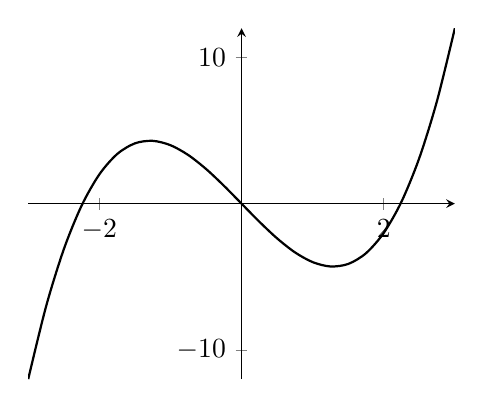
\begin{tikzpicture}
	\begin{axis} [axis lines=center]
		\addplot [domain=-3:3, smooth, thick] { x^3 - 5*x };
	\end{axis}
\end{tikzpicture}
\caption{Az $x^3-5x$ f\"uggv\'eny grafikus k\'epe PGFPLOT-al}
\end{figure}


\begin{figure}[h!]
	\centering
	\begin{tikzpicture}
		\begin{axis} [axis lines=center,xticklabels=\empty,yticklabels=\empty, xmin=-0.8,ymax=2.5,ytick style={draw=none}, xtick style={draw=none},tick,xlabel={$s$}]
			%N=6,p=3,p^*=6, p_*=5
			\addplot [domain=0:1, smooth, thick] { 1-2*x^(3) - 3*x^2  } node[midway,above right] {$\Psi$};
			\addplot[mark=*,color=red,] coordinates {(0.5,0)} node[midway,above right] {$\sigma^*$};
			\addplot[mark=*,color=red,] coordinates {(0,1)} node[midway,above left] {\scriptsize $\Psi(0)=\frac{1}{p2^{p-1}r_F^p}$};
		\end{axis}
	\end{tikzpicture}
	\caption{A $\Psi$ grafikus k\'epe}
\end{figure}
\pagebreak
\subsection{Szekvencia diagram}
 \pgfplotsset{compat=1.11}
\begin{figure}[h!]
	\centering
	\begin{tikzpicture}[
		% define a style for the dots
		dot/.style={
			draw=black,
			fill=red!90,
			circle,
			minimum size=3pt,
			inner sep=0pt,
			solid,
		},
		]
		\begin{axis}[
			xmin=-1,
			xmax=2,
			ymin=-0.5,
			ymax=3,
			axis lines=center,
			ticks=none,
			xlabel={$s$},
			xlabel style={below right},
			ylabel style={above left},
			% (moved common `addplot' options here)
			smooth,
			domain=0:2,
			samples=101,
			no markers,
			draw=black
			]
			\addplot [blue,thick] {(9*x^(5/2)-x^(11/2)-2*x^(9/2))/(1+x^(3/2)+x^(7/2)) } node [midway,above right,color=black] {$\Lambda(s)$};
			\addplot[color=red,] coordinates {(0,0)} node[midway,above left] {$\Lambda(0)$};
			% draw the dots (using the above defined style) and labels
			\draw[dashed,color=red] (0.95,0) node [dot,label=below:$s_{\rm max}$] {}-- (0.95,2.017873338) node [dot,label=above:$\Lambda(s_{\rm max})$] {};
		\end{axis}
	\end{tikzpicture}
	\caption{A $\Lambda(s)$ grafikus k\'epe}\label{LAMBDA}
\end{figure}


\begin{figure}[!h]
	\centering
	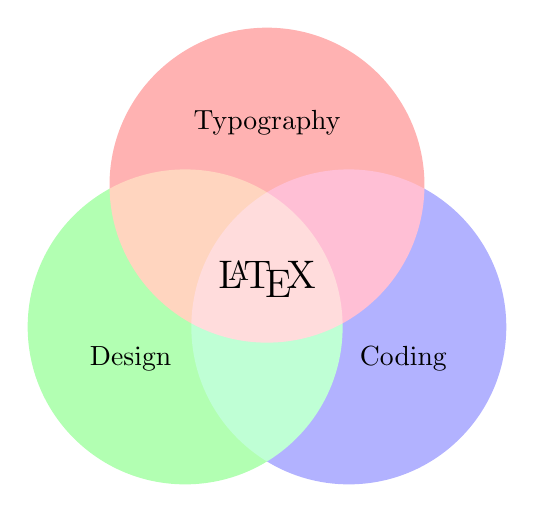
\begin{tikzpicture}
		\begin{scope}[blend group=soft light]
			\fill[red!30!white]   ( 90:1.2) circle (2);
			\fill[green!30!white] (210:1.2) circle (2);
			\fill[blue!30!white]  (330:1.2) circle (2);
		\end{scope}
		\node at ( 90:2) 	{Typography};
		\node at (210:2)  	{Design};
		\node at (330:2) {Coding};
		\node [font=\Large] {\LaTeX};
	\end{tikzpicture}
	\caption{Venn diagram TIKZ seg\'its\'egv\'evel}
\end{figure}

\begin{definition}
	Legyen $\left(X,d\right)$ \'es $\left(Y,\rho\right)$ k\'et metrikus
	t\'er, legyen $T:X\to Y$ egy lek\'epez\'es. Azt mondjuk, hogy a $T$ lek\'epez\'es
	Lipschitz tulajdons\'ag\'u, ha l\'etezik egy olyan $L>0$ sz\'am amelyre 
	\[
	\rho\left(Tx,Ty\right)\leq Ld(x,y)\;\forall x,y\in X.
	\]
	Az L sz\'amot Lipschitz \'alland\'onak nevezz\"uk.
\end{definition}

\pagebreak
Ha $T:X\to Y$ lek\'epez\'es Lipschitz tulajdons\'ag\'u, \'es az $L<1$ akkor
a $T$ oper\'atort \textbf{kontrakci\'onak} nevezz\"uk. Azt mondjuk, hogy
$x^{*}\in X$ fixpontja a $T$ oper\'atornak ha 
\[
Tx^{*}=x^{*}.
\]
\begin{theorem}{Banach f\'ele fixpontt\'etel}
	Legyen $\left(X,d\right)$ teljes metrikus t\'er \'es $T:X\to X$ lek\'epez\'es
	egy kontrakci\'o az $L<1$ \'alland\'oval. Ekkor igazak a k\"ovetkez\H{o}
	\'all\'it\'asok:
	\begin{enumerate}
		\item $T$-nek egy \'es csakis egy $x^{*}$ fixpontja.
		\item B\'arhogy v\'alasztunk meg egy $x_{0}\in X$ elemet, a $x_{k+1}=Tx_{k}$
		sorozat konvergens \'es $Tx_{k}\to x^{*},$ ahol $k$ term\'eszetes sz\'am.
		\item Igaz, hogy 
		\[
		d\left(x_{k},x^{*}\right)\leq\frac{L^{k}}{1-L}d(x_{0},Tx_{0}).
		\]
	\end{enumerate}
\end{theorem}
	% %----------------------------------------------------------------------------
\chapter*{Összefoglaló}\addcontentsline{toc}{chapter}{Összefoglaló}
%----------------------------------------------------------------------------

Dolgozatomban differenciálegyenletek megoldásával foglalkoztam, amelyet különböző programozási technológiák segítségével valósítottam meg. Először ismertettem a differenciálegyenletek numerikus megoldásának elméleti alapjait, majd megvizsgáltunk és levezettünk három numerikus módszert az Euler-, a Runge-Kutta és a Dormand-Prince módszereket. Ezek közül a mai technológiákban leginkább használatos Dormand-Prince algoritmus esetében megnéztük, hogy milyen szoftverekben tálálhatjuk meg, mint alapértelmezett differenciálegyenlet megoldó. A továbbiakban ismertettem két modellt, a leukémia betegség alap modelljét és a hullámmozgás modelljét, ezzel is kihangsúlyozva a téma fontosságát, hogy mennyire fontos az időtényező bizonyos problémák egyenleteinek medoldásánál. Ezek után részletesen is mégnéztük, hogy milyen szoftvereket alkalmaztam és alkottam a differenciálegyenletek és rendszerek megoldására. A szoftvereket két kategóriába osztotottuk fel, az első a már létező szoftverek kategóriája, a másik pedig az általam megvalósított szoftverek csoportja volt. Az első kategóriában ismertettem két technológiát, a Matlab által nyúltott ode45 beépített megoldót és a Boost könyvtárcsomagban található Odeint nevű könyvtárat. Az általam írt szofverek csoportjában négy megvalósítást mutattam be ezek a Matlab, Java, C++ és Android technológiák segítségével készültek. Emellett megnéztük, hogy mennyire hatékonyan lehet párhuzamosítani a differenciálegyenletek megoldását CUDA technológia segítségével és a grafikus kártyát (GPU-t) felhasználva. Végül kiértékeltük a tesztelés során kapott eredményeket és összehasonlítottuk a különböző programokat, kiemelve azok erősségeit és gyengéit. Majd levontuk a következtetéseket, hogy melyik technológia irányában érdemes tovább haladni és melyik az, amelyikkel nem éri meg foglalkozni.

Jövőbeli terveimet illetően szeretnék jobban elmerülni a GPU-n történő differenciálegyenletek megoldásának módszereiben, valamint ezek alkalmazását kipróbálni és tanulmányozni a parciális differenciálegyenletek területén (PDE). Továbbá érdemesnek tartom a C++ szoftver továbbfejlesztését és egy differenciálegyenlet megoldó könyvtár megalkotását, amely ingyenesen használható és nyílt forráskódú lenne.

% Koszonetnyilvanitas
%~~~~~~~~~~~~~~~~~~~~~~~~~~~~~~~~~~~~~~~~~~~~~~~~~~~~~~~~~~~~~~~~~~~~~~~~~~~~~~~~~~~~~~
	% %----------------------------------------------------------------------------
\chapter*{\koszonetnyilvanitas}\addcontentsline{toc}{chapter}{\koszonetnyilvanitas}
%----------------------------------------------------------------------------

Ez nem kötelező, akár törölhető is. Ha a szerző szükségét érzi, itt lehet köszönetet nyilvánítani azoknak, akik hozzájárultak munkájukkal ahhoz, hogy a hallgató a szakdolgozatban vagy diplomamunkában leírt feladatokat sikeresen elvégezze. A konzulensnek való köszönetnyilvánítás sem kötelező, a konzulensnek hivatalosan is dolga, hogy a hallgatót konzultálja.


% Tablazatok es abrak jegyzeke (EZ NEM KOTELEZO)
%~~~~~~~~~~~~~~~~~~~~~~~~~~~~~~~~~~~~~~~~~~~~~~~~~~~~~~~~~~~~~~~~~~~~~~~~~~~~~~~~~~~~~~
	% \listoffigures\addcontentsline{toc}{chapter}{\abrakjegyzeke}
	% \listoftables\addcontentsline{toc}{chapter}{\tablazatokjegyzeke}


% Bibliography
%~~~~~~~~~~~~~~~~~~~~~~~~~~~~~~~~~~~~~~~~~~~~~~~~~~~~~~~~~~~~~~~~~~~~~~~~~~~~~~~~~~~~~~
	\bibliographystyle{plain}
	\bibliography{cite}
	
% Appendix
%~~~~~~~~~~~~~~~~~~~~~~~~~~~~~~~~~~~~~~~~~~~~~~~~~~~~~~~~~~~~~~~~~~~~~~~~~~~~~~~~~~~~~~
	% %----------------------------------------------------------------------------
\appendix
%----------------------------------------------------------------------------
\chapter*{\fuggelek}\addcontentsline{toc}{chapter}{\fuggelek}
\setcounter{chapter}{6}  % a fofejezet-szamlalo az angol ABC 6. betuje (F) lesz
\setcounter{equation}{0} % a fofejezet-szamlalo az angol ABC 6. betuje (F) lesz
\numberwithin{equation}{section}
\numberwithin{figure}{section}
\numberwithin{lstlisting}{section}
%\numberwithin{tabular}{section}

%----------------------------------------------------------------------------
\section{A TeXstudio felülete}
%----------------------------------------------------------------------------
\begin{figure}[!ht]
\centering
\includegraphics[width=150mm, keepaspectratio]{images/texstudio}
\caption{A TeXstudio \LaTeX-szerkesztő.} 
\end{figure}

%----------------------------------------------------------------------------
\clearpage\section{Válasz az ,,Élet, a világmindenség, meg minden'' kérdésére}
%----------------------------------------------------------------------------
A Pitagorasz-tételből levezetve
\begin{align}
c^2=a^2+b^2=42.
\end{align}
A Faraday-indukciós törvényből levezetve
\begin{align}
\rot E=-\frac{dB}{dt}\hspace{1cm}\longrightarrow \hspace{1cm}
U_i=\oint\limits_\mathbf{L}{\mathbf{E}\mathbf{dl}}=-\frac{d}{dt}\int\limits_A{\mathbf{B}\mathbf{da}}=42.
\end{align}







\label{page:last}
\end{document}
